\documentclass[twoside]{book}

% Packages required by doxygen
\usepackage{fixltx2e}
\usepackage{calc}
\usepackage{doxygen}
\usepackage[export]{adjustbox} % also loads graphicx
\usepackage{graphicx}
\usepackage[utf8]{inputenc}
\usepackage{makeidx}
\usepackage{multicol}
\usepackage{multirow}
\PassOptionsToPackage{warn}{textcomp}
\usepackage{textcomp}
\usepackage[nointegrals]{wasysym}
\usepackage[table]{xcolor}

% Font selection
\usepackage[T1]{fontenc}
\usepackage[scaled=.90]{helvet}
\usepackage{courier}
\usepackage{amssymb}
\usepackage{sectsty}
\renewcommand{\familydefault}{\sfdefault}
\allsectionsfont{%
  \fontseries{bc}\selectfont%
  \color{darkgray}%
}
\renewcommand{\DoxyLabelFont}{%
  \fontseries{bc}\selectfont%
  \color{darkgray}%
}
\newcommand{\+}{\discretionary{\mbox{\scriptsize$\hookleftarrow$}}{}{}}

% Page & text layout
\usepackage{geometry}
\geometry{%
  a4paper,%
  top=2.5cm,%
  bottom=2.5cm,%
  left=2.5cm,%
  right=2.5cm%
}
\tolerance=750
\hfuzz=15pt
\hbadness=750
\setlength{\emergencystretch}{15pt}
\setlength{\parindent}{0cm}
\setlength{\parskip}{3ex plus 2ex minus 2ex}
\makeatletter
\renewcommand{\paragraph}{%
  \@startsection{paragraph}{4}{0ex}{-1.0ex}{1.0ex}{%
    \normalfont\normalsize\bfseries\SS@parafont%
  }%
}
\renewcommand{\subparagraph}{%
  \@startsection{subparagraph}{5}{0ex}{-1.0ex}{1.0ex}{%
    \normalfont\normalsize\bfseries\SS@subparafont%
  }%
}
\makeatother

% Headers & footers
\usepackage{fancyhdr}
\pagestyle{fancyplain}
\fancyhead[LE]{\fancyplain{}{\bfseries\thepage}}
\fancyhead[CE]{\fancyplain{}{}}
\fancyhead[RE]{\fancyplain{}{\bfseries\leftmark}}
\fancyhead[LO]{\fancyplain{}{\bfseries\rightmark}}
\fancyhead[CO]{\fancyplain{}{}}
\fancyhead[RO]{\fancyplain{}{\bfseries\thepage}}
\fancyfoot[LE]{\fancyplain{}{}}
\fancyfoot[CE]{\fancyplain{}{}}
\fancyfoot[RE]{\fancyplain{}{\bfseries\scriptsize Generated by Doxygen }}
\fancyfoot[LO]{\fancyplain{}{\bfseries\scriptsize Generated by Doxygen }}
\fancyfoot[CO]{\fancyplain{}{}}
\fancyfoot[RO]{\fancyplain{}{}}
\renewcommand{\footrulewidth}{0.4pt}
\renewcommand{\chaptermark}[1]{%
  \markboth{#1}{}%
}
\renewcommand{\sectionmark}[1]{%
  \markright{\thesection\ #1}%
}

% Indices & bibliography
\usepackage{natbib}
\usepackage[titles]{tocloft}
\setcounter{tocdepth}{3}
\setcounter{secnumdepth}{5}
\makeindex

% Hyperlinks (required, but should be loaded last)
\usepackage{ifpdf}
\ifpdf
  \usepackage[pdftex,pagebackref=true]{hyperref}
\else
  \usepackage[ps2pdf,pagebackref=true]{hyperref}
\fi
\hypersetup{%
  colorlinks=true,%
  linkcolor=blue,%
  citecolor=blue,%
  unicode%
}

% Custom commands
\newcommand{\clearemptydoublepage}{%
  \newpage{\pagestyle{empty}\cleardoublepage}%
}

\usepackage{caption}
\captionsetup{labelsep=space,justification=centering,font={bf},singlelinecheck=off,skip=4pt,position=top}

%===== C O N T E N T S =====

\begin{document}

% Titlepage & ToC
\hypersetup{pageanchor=false,
             bookmarksnumbered=true,
             pdfencoding=unicode
            }
\pagenumbering{alph}
\begin{titlepage}
\vspace*{7cm}
\begin{center}%
{\Large Let\textquotesingle{}s play N\+FL football }\\
\vspace*{1cm}
{\large Generated by Doxygen 1.8.13}\\
\end{center}
\end{titlepage}
\clearemptydoublepage
\pagenumbering{roman}
\tableofcontents
\clearemptydoublepage
\pagenumbering{arabic}
\hypersetup{pageanchor=true}

%--- Begin generated contents ---
\chapter{N\+F\+L-\/\+Football-\/\+Project}
\label{md__r_e_a_d_m_e}
\Hypertarget{md__r_e_a_d_m_e}
C\+S1D Project 2 Fall 2017

\section*{Waffle.\+io}

\href{https://waffle.io/OneEcho/NFL-Football-Project}{\tt https\+://waffle.\+io/\+One\+Echo/\+N\+F\+L-\/\+Football-\/\+Project} 
\chapter{Hierarchical Index}
\section{Class Hierarchy}
This inheritance list is sorted roughly, but not completely, alphabetically\+:\begin{DoxyCompactList}
\item \contentsline{section}{Cart}{\pageref{class_cart}}{}
\item \contentsline{section}{college\+Stadium\+Pair}{\pageref{structcollege_stadium_pair}}{}
\item \contentsline{section}{Edge}{\pageref{struct_edge}}{}
\item \contentsline{section}{Graph}{\pageref{class_graph}}{}
\item \contentsline{section}{Map}{\pageref{class_map}}{}
\item \contentsline{section}{Map\+Node}{\pageref{class_map_node}}{}
\item \contentsline{section}{Purchase}{\pageref{class_purchase}}{}
\item Q\+Dialog\begin{DoxyCompactList}
\item \contentsline{section}{modifysouvenirs}{\pageref{classmodifysouvenirs}}{}
\item \contentsline{section}{modify\+Stadium\+Info}{\pageref{classmodify_stadium_info}}{}
\end{DoxyCompactList}
\item Q\+Main\+Window\begin{DoxyCompactList}
\item \contentsline{section}{admin\+Window}{\pageref{classadmin_window}}{}
\item \contentsline{section}{Main\+Window}{\pageref{class_main_window}}{}
\end{DoxyCompactList}
\item Q\+Sql\+Database\begin{DoxyCompactList}
\item \contentsline{section}{Database}{\pageref{class_database}}{}
\end{DoxyCompactList}
\item \contentsline{section}{Souvenir}{\pageref{class_souvenir}}{}
\item \contentsline{section}{Graph\+:\+:traversal\+Info}{\pageref{struct_graph_1_1traversal_info}}{}
\item \contentsline{section}{Ui\+\_\+admin\+Window}{\pageref{class_ui__admin_window}}{}
\begin{DoxyCompactList}
\item \contentsline{section}{Ui\+:\+:admin\+Window}{\pageref{class_ui_1_1admin_window}}{}
\end{DoxyCompactList}
\item \contentsline{section}{Ui\+\_\+\+Main\+Window}{\pageref{class_ui___main_window}}{}
\begin{DoxyCompactList}
\item \contentsline{section}{Ui\+:\+:Main\+Window}{\pageref{class_ui_1_1_main_window}}{}
\end{DoxyCompactList}
\item \contentsline{section}{Ui\+\_\+modifysouvenirs}{\pageref{class_ui__modifysouvenirs}}{}
\begin{DoxyCompactList}
\item \contentsline{section}{Ui\+:\+:modifysouvenirs}{\pageref{class_ui_1_1modifysouvenirs}}{}
\end{DoxyCompactList}
\item \contentsline{section}{Ui\+\_\+modify\+Stadium\+Info}{\pageref{class_ui__modify_stadium_info}}{}
\begin{DoxyCompactList}
\item \contentsline{section}{Ui\+:\+:modify\+Stadium\+Info}{\pageref{class_ui_1_1modify_stadium_info}}{}
\end{DoxyCompactList}
\item \contentsline{section}{Vertex}{\pageref{struct_vertex}}{}
\end{DoxyCompactList}

\chapter{Class Index}
\section{Class List}
Here are the classes, structs, unions and interfaces with brief descriptions\+:\begin{DoxyCompactList}
\item\contentsline{section}{\hyperlink{classadmin_window}{admin\+Window} }{\pageref{classadmin_window}}{}
\item\contentsline{section}{\hyperlink{class_ui_1_1admin_window}{Ui\+::admin\+Window} }{\pageref{class_ui_1_1admin_window}}{}
\item\contentsline{section}{\hyperlink{class_cart}{Cart} }{\pageref{class_cart}}{}
\item\contentsline{section}{\hyperlink{structcollege_stadium_pair}{college\+Stadium\+Pair} }{\pageref{structcollege_stadium_pair}}{}
\item\contentsline{section}{\hyperlink{class_database}{Database} }{\pageref{class_database}}{}
\item\contentsline{section}{\hyperlink{struct_edge}{Edge} \\*Used to represent a \hyperlink{struct_edge}{Edge} for the graph class }{\pageref{struct_edge}}{}
\item\contentsline{section}{\hyperlink{class_graph}{Graph} \\*Used to represent a graph data structure }{\pageref{class_graph}}{}
\item\contentsline{section}{\hyperlink{class_main_window}{Main\+Window} }{\pageref{class_main_window}}{}
\item\contentsline{section}{\hyperlink{class_ui_1_1_main_window}{Ui\+::\+Main\+Window} }{\pageref{class_ui_1_1_main_window}}{}
\item\contentsline{section}{\hyperlink{class_map}{Map} }{\pageref{class_map}}{}
\item\contentsline{section}{\hyperlink{class_map_node}{Map\+Node} }{\pageref{class_map_node}}{}
\item\contentsline{section}{\hyperlink{class_ui_1_1modifysouvenirs}{Ui\+::modifysouvenirs} }{\pageref{class_ui_1_1modifysouvenirs}}{}
\item\contentsline{section}{\hyperlink{classmodifysouvenirs}{modifysouvenirs} }{\pageref{classmodifysouvenirs}}{}
\item\contentsline{section}{\hyperlink{class_ui_1_1modify_stadium_info}{Ui\+::modify\+Stadium\+Info} }{\pageref{class_ui_1_1modify_stadium_info}}{}
\item\contentsline{section}{\hyperlink{classmodify_stadium_info}{modify\+Stadium\+Info} }{\pageref{classmodify_stadium_info}}{}
\item\contentsline{section}{\hyperlink{class_purchase}{Purchase} }{\pageref{class_purchase}}{}
\item\contentsline{section}{\hyperlink{class_souvenir}{Souvenir} }{\pageref{class_souvenir}}{}
\item\contentsline{section}{\hyperlink{struct_graph_1_1traversal_info}{Graph\+::traversal\+Info} }{\pageref{struct_graph_1_1traversal_info}}{}
\item\contentsline{section}{\hyperlink{class_ui__admin_window}{Ui\+\_\+admin\+Window} }{\pageref{class_ui__admin_window}}{}
\item\contentsline{section}{\hyperlink{class_ui___main_window}{Ui\+\_\+\+Main\+Window} }{\pageref{class_ui___main_window}}{}
\item\contentsline{section}{\hyperlink{class_ui__modifysouvenirs}{Ui\+\_\+modifysouvenirs} }{\pageref{class_ui__modifysouvenirs}}{}
\item\contentsline{section}{\hyperlink{class_ui__modify_stadium_info}{Ui\+\_\+modify\+Stadium\+Info} }{\pageref{class_ui__modify_stadium_info}}{}
\item\contentsline{section}{\hyperlink{struct_vertex}{Vertex} \\*Used to represent a \hyperlink{struct_vertex}{Vertex} for the graph class }{\pageref{struct_vertex}}{}
\end{DoxyCompactList}

\chapter{Class Documentation}
\hypertarget{classadmin_window}{}\section{admin\+Window Class Reference}
\label{classadmin_window}\index{admin\+Window@{admin\+Window}}


Inheritance diagram for admin\+Window\+:
\nopagebreak
\begin{figure}[H]
\begin{center}
\leavevmode
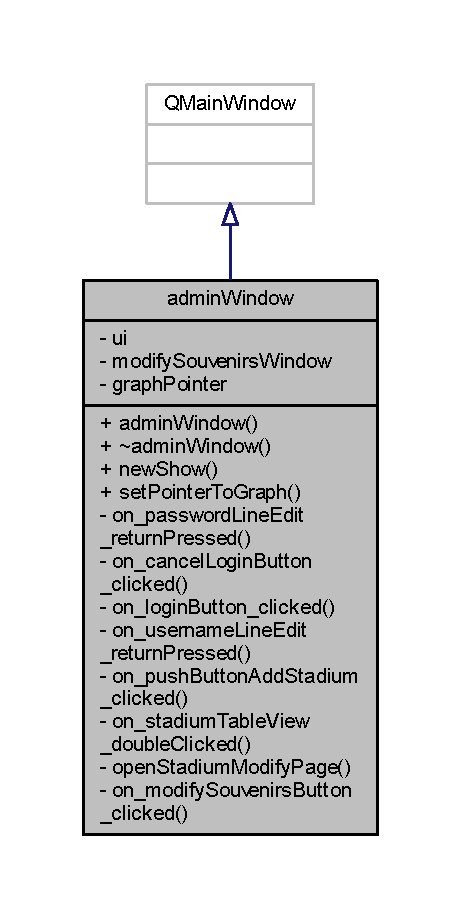
\includegraphics[width=221pt]{classadmin_window__inherit__graph}
\end{center}
\end{figure}


Collaboration diagram for admin\+Window\+:
\nopagebreak
\begin{figure}[H]
\begin{center}
\leavevmode
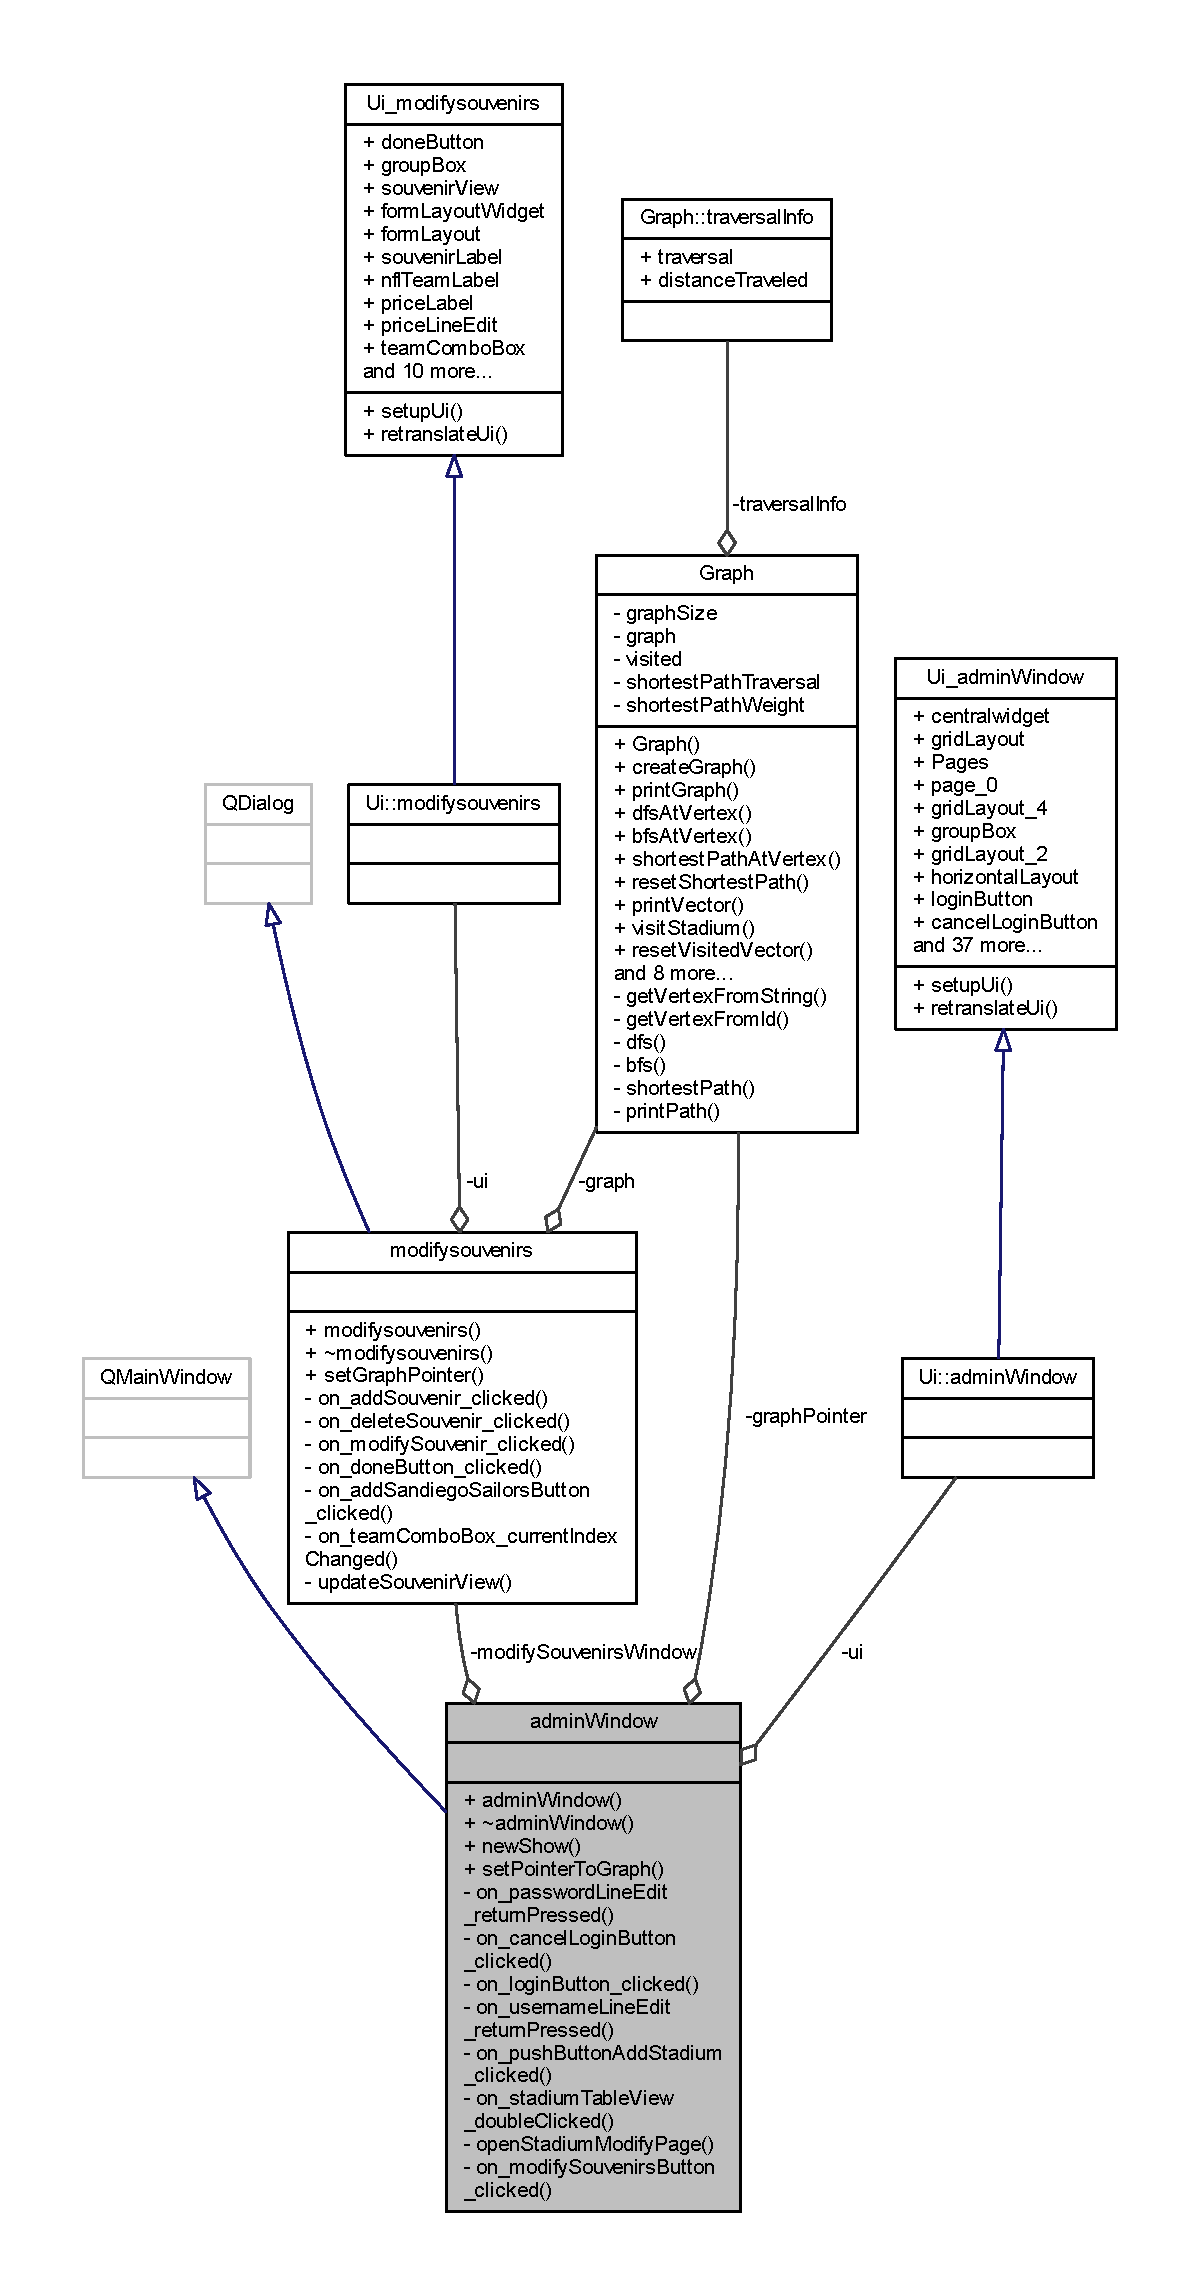
\includegraphics[height=550pt]{classadmin_window__coll__graph}
\end{center}
\end{figure}
\subsection*{Public Member Functions}
\begin{DoxyCompactItemize}
\item 
\mbox{\Hypertarget{classadmin_window_aa87a28958c1a314408df44e88c886ac5}\label{classadmin_window_aa87a28958c1a314408df44e88c886ac5}} 
{\bfseries admin\+Window} (Q\+Widget $\ast$parent=0)
\item 
\mbox{\Hypertarget{classadmin_window_a82510bb37f35a28caa9049a127b047fe}\label{classadmin_window_a82510bb37f35a28caa9049a127b047fe}} 
void {\bfseries new\+Show} ()
\item 
\mbox{\Hypertarget{classadmin_window_a0a12fa17f4293753eeb62137c06d7773}\label{classadmin_window_a0a12fa17f4293753eeb62137c06d7773}} 
void {\bfseries set\+Pointer\+To\+Graph} (\hyperlink{class_graph}{Graph} $\ast$p)
\end{DoxyCompactItemize}
\subsection*{Private Slots}
\begin{DoxyCompactItemize}
\item 
\mbox{\Hypertarget{classadmin_window_a5103280c9df5284396543abbcfdfb9b0}\label{classadmin_window_a5103280c9df5284396543abbcfdfb9b0}} 
void {\bfseries on\+\_\+password\+Line\+Edit\+\_\+return\+Pressed} ()
\item 
\mbox{\Hypertarget{classadmin_window_ababda5dfc198c2d5a740a69439438309}\label{classadmin_window_ababda5dfc198c2d5a740a69439438309}} 
void {\bfseries on\+\_\+cancel\+Login\+Button\+\_\+clicked} ()
\item 
\mbox{\Hypertarget{classadmin_window_ae2fb0ef45daf7c5dc9c1be3c8d70ddfd}\label{classadmin_window_ae2fb0ef45daf7c5dc9c1be3c8d70ddfd}} 
void {\bfseries on\+\_\+login\+Button\+\_\+clicked} ()
\item 
\mbox{\Hypertarget{classadmin_window_acda88c79d0311b10ca14365c758806b1}\label{classadmin_window_acda88c79d0311b10ca14365c758806b1}} 
void {\bfseries on\+\_\+username\+Line\+Edit\+\_\+return\+Pressed} ()
\item 
\mbox{\Hypertarget{classadmin_window_a4335abd3c293747b320e7b33daa97ac9}\label{classadmin_window_a4335abd3c293747b320e7b33daa97ac9}} 
void {\bfseries on\+\_\+push\+Button\+Add\+Stadium\+\_\+clicked} ()
\item 
\mbox{\Hypertarget{classadmin_window_af4d34bb5631807d4fdec44be2aba6f43}\label{classadmin_window_af4d34bb5631807d4fdec44be2aba6f43}} 
void {\bfseries on\+\_\+stadium\+Table\+View\+\_\+double\+Clicked} (const Q\+Model\+Index \&index)
\item 
\mbox{\Hypertarget{classadmin_window_acce92c02ca24ae9d6f3aea46ade5c32f}\label{classadmin_window_acce92c02ca24ae9d6f3aea46ade5c32f}} 
void {\bfseries open\+Stadium\+Modify\+Page} ()
\item 
\mbox{\Hypertarget{classadmin_window_af2ca6f61fc6981b6ea720993642fd7b6}\label{classadmin_window_af2ca6f61fc6981b6ea720993642fd7b6}} 
void {\bfseries on\+\_\+modify\+Souvenirs\+Button\+\_\+clicked} ()
\end{DoxyCompactItemize}
\subsection*{Private Attributes}
\begin{DoxyCompactItemize}
\item 
\mbox{\Hypertarget{classadmin_window_a0588ac6ffce4f1564831df57a6fde502}\label{classadmin_window_a0588ac6ffce4f1564831df57a6fde502}} 
\hyperlink{class_ui_1_1admin_window}{Ui\+::admin\+Window} $\ast$ {\bfseries ui}
\item 
\mbox{\Hypertarget{classadmin_window_a70c04791ef7eed9cd56feb4bde28112a}\label{classadmin_window_a70c04791ef7eed9cd56feb4bde28112a}} 
\hyperlink{classmodifysouvenirs}{modifysouvenirs} $\ast$ {\bfseries modify\+Souvenirs\+Window}
\item 
\mbox{\Hypertarget{classadmin_window_a937bdf631bf80712039ef52bb89159ea}\label{classadmin_window_a937bdf631bf80712039ef52bb89159ea}} 
\hyperlink{class_graph}{Graph} $\ast$ {\bfseries graph\+Pointer}
\end{DoxyCompactItemize}


The documentation for this class was generated from the following files\+:\begin{DoxyCompactItemize}
\item 
adminwindow.\+h\item 
adminwindow.\+cpp\end{DoxyCompactItemize}

\hypertarget{class_ui_1_1admin_window}{}\section{Ui\+:\+:admin\+Window Class Reference}
\label{class_ui_1_1admin_window}\index{Ui\+::admin\+Window@{Ui\+::admin\+Window}}
Inheritance diagram for Ui\+:\+:admin\+Window\+:\begin{figure}[H]
\begin{center}
\leavevmode
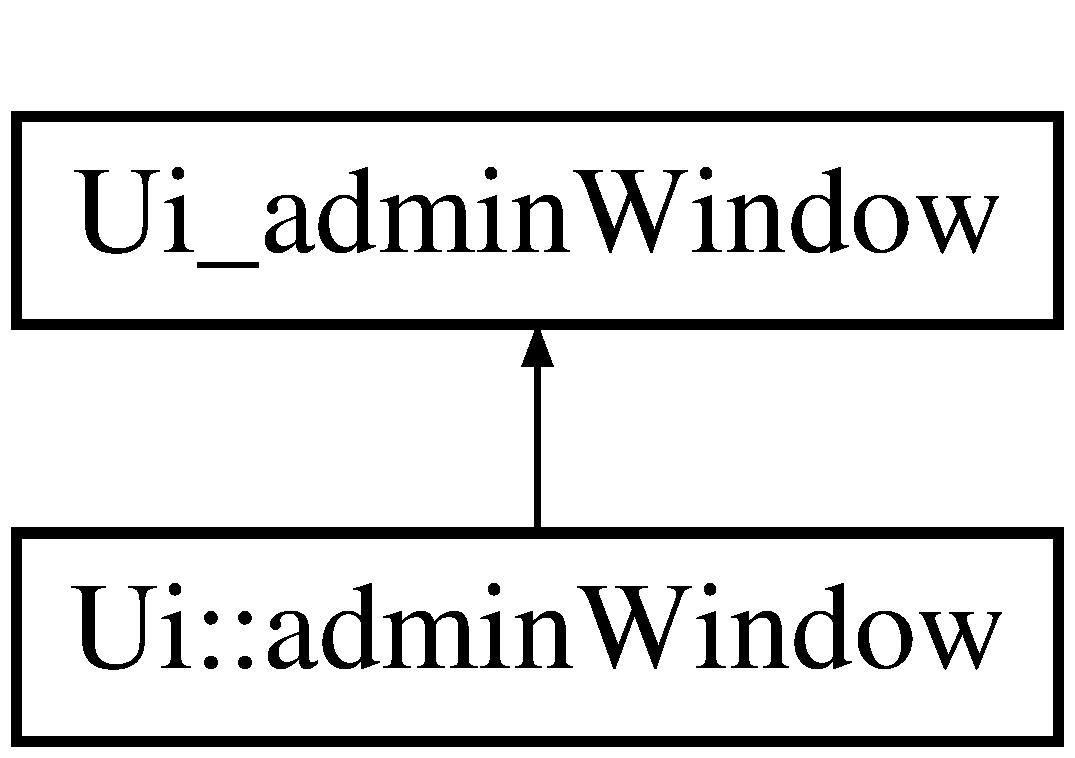
\includegraphics[height=2.000000cm]{class_ui_1_1admin_window}
\end{center}
\end{figure}
\subsection*{Additional Inherited Members}


The documentation for this class was generated from the following file\+:\begin{DoxyCompactItemize}
\item 
ui\+\_\+adminwindow.\+h\end{DoxyCompactItemize}

\hypertarget{class_cart}{}\section{Cart Class Reference}
\label{class_cart}\index{Cart@{Cart}}
\subsection*{Public Member Functions}
\begin{DoxyCompactItemize}
\item 
\mbox{\Hypertarget{class_cart_a2260991ab57f2d95e17e977e4c183fdd}\label{class_cart_a2260991ab57f2d95e17e977e4c183fdd}} 
void {\bfseries add\+Purchase} (double price, int quantity, Q\+String item\+Name, Q\+String team\+Nmae)
\item 
\mbox{\Hypertarget{class_cart_a2299824d255f3110ad5eda5bfbd1b3ac}\label{class_cart_a2299824d255f3110ad5eda5bfbd1b3ac}} 
double {\bfseries get\+Total\+Spent} ()
\item 
\mbox{\Hypertarget{class_cart_a45873b2f5d9913f9de39599d8ab25a12}\label{class_cart_a45873b2f5d9913f9de39599d8ab25a12}} 
double {\bfseries get\+Total\+Spent\+At} (Q\+String stadium)
\item 
\mbox{\Hypertarget{class_cart_abced3b2b64a6800abb3e37b62496d2e5}\label{class_cart_abced3b2b64a6800abb3e37b62496d2e5}} 
int {\bfseries get\+Quantity} (int i)
\item 
\mbox{\Hypertarget{class_cart_ad4906647eb9e958121d301f4aa9eb215}\label{class_cart_ad4906647eb9e958121d301f4aa9eb215}} 
Q\+String {\bfseries get\+Souvenir\+Name} (int i)
\item 
\mbox{\Hypertarget{class_cart_a2d0efd1dac0bcbe20c739dfdc2db8d05}\label{class_cart_a2d0efd1dac0bcbe20c739dfdc2db8d05}} 
double {\bfseries get\+Total\+Price} (int i)
\item 
\mbox{\Hypertarget{class_cart_ae084fb0f5de20ded9e938dc28676daea}\label{class_cart_ae084fb0f5de20ded9e938dc28676daea}} 
Q\+String {\bfseries get\+Team\+Name} (int i)
\item 
\mbox{\Hypertarget{class_cart_ac89333c3766ab987cad13fc430407b78}\label{class_cart_ac89333c3766ab987cad13fc430407b78}} 
int {\bfseries size} ()
\end{DoxyCompactItemize}
\subsection*{Private Attributes}
\begin{DoxyCompactItemize}
\item 
\mbox{\Hypertarget{class_cart_a546a0df14f71469925c0cf008667983c}\label{class_cart_a546a0df14f71469925c0cf008667983c}} 
Q\+Vector$<$ \hyperlink{class_purchase}{Purchase} $>$ {\bfseries souvenirs}
\end{DoxyCompactItemize}


The documentation for this class was generated from the following files\+:\begin{DoxyCompactItemize}
\item 
cart.\+h\item 
cart.\+cpp\end{DoxyCompactItemize}

\hypertarget{structcollege_stadium_pair}{}\section{college\+Stadium\+Pair Struct Reference}
\label{structcollege_stadium_pair}\index{college\+Stadium\+Pair@{college\+Stadium\+Pair}}


Collaboration diagram for college\+Stadium\+Pair\+:
\nopagebreak
\begin{figure}[H]
\begin{center}
\leavevmode
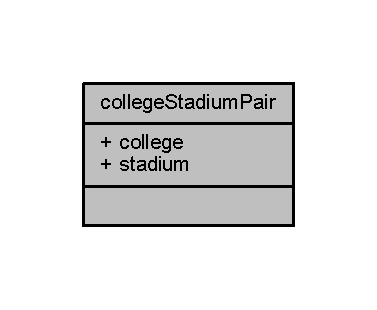
\includegraphics[width=181pt]{structcollege_stadium_pair__coll__graph}
\end{center}
\end{figure}
\subsection*{Public Attributes}
\begin{DoxyCompactItemize}
\item 
\mbox{\Hypertarget{structcollege_stadium_pair_a77ca4473825d5cd624b735a458b307bb}\label{structcollege_stadium_pair_a77ca4473825d5cd624b735a458b307bb}} 
Q\+String {\bfseries college}
\item 
\mbox{\Hypertarget{structcollege_stadium_pair_a670f797a70b4d32b10c49414aada09ee}\label{structcollege_stadium_pair_a670f797a70b4d32b10c49414aada09ee}} 
Q\+String {\bfseries stadium}
\end{DoxyCompactItemize}


The documentation for this struct was generated from the following file\+:\begin{DoxyCompactItemize}
\item 
mainwindow.\+h\end{DoxyCompactItemize}

\hypertarget{class_database}{}\section{Database Class Reference}
\label{class_database}\index{Database@{Database}}


{\ttfamily \#include $<$database.\+h$>$}



Inheritance diagram for Database\+:
\nopagebreak
\begin{figure}[H]
\begin{center}
\leavevmode
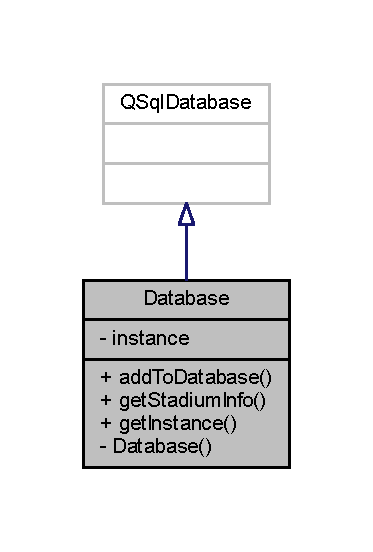
\includegraphics[width=179pt]{class_database__inherit__graph}
\end{center}
\end{figure}


Collaboration diagram for Database\+:
\nopagebreak
\begin{figure}[H]
\begin{center}
\leavevmode
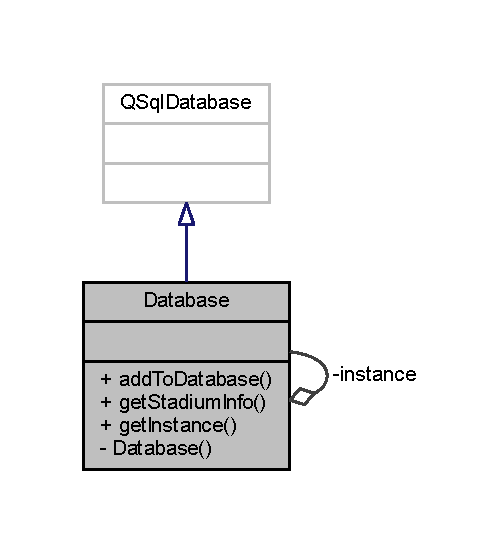
\includegraphics[width=240pt]{class_database__coll__graph}
\end{center}
\end{figure}
\subsection*{Public Member Functions}
\begin{DoxyCompactItemize}
\item 
\mbox{\Hypertarget{class_database_a76a9b0363174bdd6c70a052a088cfaf8}\label{class_database_a76a9b0363174bdd6c70a052a088cfaf8}} 
void {\bfseries add\+To\+Database} ()
\item 
\mbox{\Hypertarget{class_database_a94df9dbb511243da5a288eefc17348cb}\label{class_database_a94df9dbb511243da5a288eefc17348cb}} 
Q\+Sql\+Query\+Model $\ast$ {\bfseries get\+Stadium\+Info} ()
\end{DoxyCompactItemize}
\subsection*{Static Public Member Functions}
\begin{DoxyCompactItemize}
\item 
static \hyperlink{class_database}{Database} $\ast$ \hyperlink{class_database_a5a3b028f980a577ea0b809eb92312761}{get\+Instance} ()
\end{DoxyCompactItemize}
\subsection*{Private Member Functions}
\begin{DoxyCompactItemize}
\item 
\hyperlink{class_database_a4703c80e6969d33565ea340f768fdadf}{Database} ()
\end{DoxyCompactItemize}
\subsection*{Static Private Attributes}
\begin{DoxyCompactItemize}
\item 
static \hyperlink{class_database}{Database} $\ast$ \hyperlink{class_database_a5926460fe1c15c95d470fcde637f8d22}{instance} = nullptr
\end{DoxyCompactItemize}


\subsection{Detailed Description}
Our database is a singleton because we dont want accidental copies 

\subsection{Constructor \& Destructor Documentation}
\mbox{\Hypertarget{class_database_a4703c80e6969d33565ea340f768fdadf}\label{class_database_a4703c80e6969d33565ea340f768fdadf}} 
\index{Database@{Database}!Database@{Database}}
\index{Database@{Database}!Database@{Database}}
\subsubsection{\texorpdfstring{Database()}{Database()}}
{\footnotesize\ttfamily Database\+::\+Database (\begin{DoxyParamCaption}{ }\end{DoxyParamCaption})\hspace{0.3cm}{\ttfamily [private]}}

private constructor so it cannot be accessed publicly

//\+This is our private constructor This ensures that our database is a singleton. We only need one copy of the database add the path to the \hyperlink{class_database}{Database} inside quotes

add th path to the \hyperlink{class_database}{Database} inside quotes 

\subsection{Member Function Documentation}
\mbox{\Hypertarget{class_database_a5a3b028f980a577ea0b809eb92312761}\label{class_database_a5a3b028f980a577ea0b809eb92312761}} 
\index{Database@{Database}!get\+Instance@{get\+Instance}}
\index{get\+Instance@{get\+Instance}!Database@{Database}}
\subsubsection{\texorpdfstring{get\+Instance()}{getInstance()}}
{\footnotesize\ttfamily \hyperlink{class_database}{Database} $\ast$ Database\+::get\+Instance (\begin{DoxyParamCaption}{ }\end{DoxyParamCaption})\hspace{0.3cm}{\ttfamily [static]}}


\begin{DoxyItemize}
\item \begin{DoxyReturn}{Returns}

\end{DoxyReturn}

\end{DoxyItemize}if the instance is still a nullptr

create a new instance

if the instance exists, it\textquotesingle{}ll return a copy of the isntance Or if the new instance has been made, it will return that 

\subsection{Member Data Documentation}
\mbox{\Hypertarget{class_database_a5926460fe1c15c95d470fcde637f8d22}\label{class_database_a5926460fe1c15c95d470fcde637f8d22}} 
\index{Database@{Database}!instance@{instance}}
\index{instance@{instance}!Database@{Database}}
\subsubsection{\texorpdfstring{instance}{instance}}
{\footnotesize\ttfamily \hyperlink{class_database}{Database} $\ast$ Database\+::instance = nullptr\hspace{0.3cm}{\ttfamily [static]}, {\ttfamily [private]}}

static variable of our singleton instance

This ensures that our database is a singleton. We only need one copy of the database 

The documentation for this class was generated from the following files\+:\begin{DoxyCompactItemize}
\item 
database.\+h\item 
database.\+cpp\end{DoxyCompactItemize}

\hypertarget{struct_edge}{}\section{Edge Struct Reference}
\label{struct_edge}\index{Edge@{Edge}}


Used to represent a \hyperlink{struct_edge}{Edge} for the graph class.  




{\ttfamily \#include $<$graph.\+h$>$}

\subsection*{Public Attributes}
\begin{DoxyCompactItemize}
\item 
\mbox{\Hypertarget{struct_edge_a60f98913cc48bc254567cdb52d592e1c}\label{struct_edge_a60f98913cc48bc254567cdb52d592e1c}} 
\hyperlink{struct_vertex}{Vertex} $\ast$ {\bfseries connected\+Vertex}
\item 
\mbox{\Hypertarget{struct_edge_a4d58e1f4de38fa55549497175981ebab}\label{struct_edge_a4d58e1f4de38fa55549497175981ebab}} 
int {\bfseries weight}
\end{DoxyCompactItemize}


\subsection{Detailed Description}
Used to represent a \hyperlink{struct_edge}{Edge} for the graph class. 

This struct represents a edge for the graph. It uses a pointer variable to hold the connected vertex and integer variable for the weight. 

The documentation for this struct was generated from the following file\+:\begin{DoxyCompactItemize}
\item 
graph.\+h\end{DoxyCompactItemize}

\hypertarget{class_graph}{}\section{Graph Class Reference}
\label{class_graph}\index{Graph@{Graph}}


Used to represent a graph data structure.  




{\ttfamily \#include $<$graph.\+h$>$}



Collaboration diagram for Graph\+:\nopagebreak
\begin{figure}[H]
\begin{center}
\leavevmode
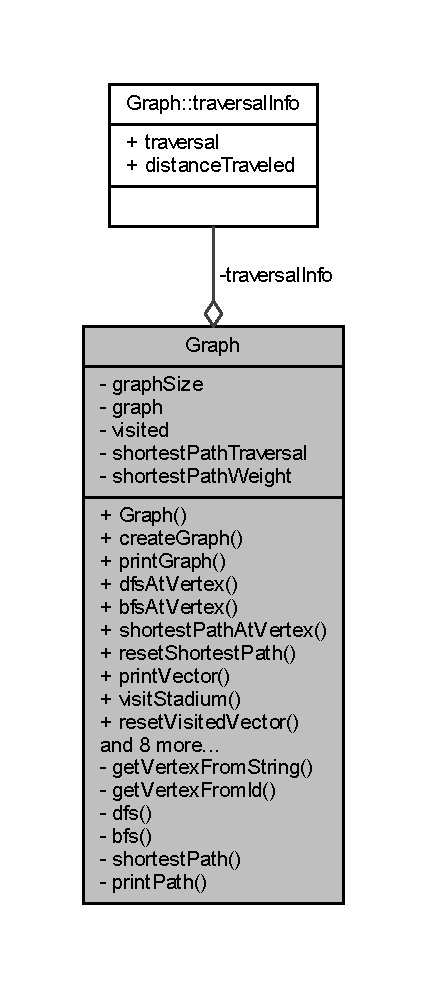
\includegraphics[width=205pt]{class_graph__coll__graph}
\end{center}
\end{figure}
\subsection*{Classes}
\begin{DoxyCompactItemize}
\item 
struct \hyperlink{struct_graph_1_1traversal_info}{traversal\+Info}
\end{DoxyCompactItemize}
\subsection*{Public Member Functions}
\begin{DoxyCompactItemize}
\item 
\mbox{\Hypertarget{class_graph_ae4c72b8ac4d693c49800a4c7e273654f}\label{class_graph_ae4c72b8ac4d693c49800a4c7e273654f}} 
\hyperlink{class_graph_ae4c72b8ac4d693c49800a4c7e273654f}{Graph} ()
\begin{DoxyCompactList}\small\item\em Default constructor. \end{DoxyCompactList}\item 
\mbox{\Hypertarget{class_graph_a33a161c48acd375508bbf95e697bf453}\label{class_graph_a33a161c48acd375508bbf95e697bf453}} 
void \hyperlink{class_graph_a33a161c48acd375508bbf95e697bf453}{create\+Graph} ()
\begin{DoxyCompactList}\small\item\em Creates the graph using information from the database. \end{DoxyCompactList}\item 
\mbox{\Hypertarget{class_graph_a5ac05db53839e72af76cdb2bafe88b77}\label{class_graph_a5ac05db53839e72af76cdb2bafe88b77}} 
void \hyperlink{class_graph_a5ac05db53839e72af76cdb2bafe88b77}{print\+Graph} ()
\begin{DoxyCompactList}\small\item\em Prints the graph. \end{DoxyCompactList}\item 
void \hyperlink{class_graph_a2a65cf186c6fb2b2cc729c5912f64c72}{dfs\+At\+Vertex} (Q\+String label)
\begin{DoxyCompactList}\small\item\em Performs a D\+FS traversal. \end{DoxyCompactList}\item 
void \hyperlink{class_graph_a11be2135c68163907d6bb1a268316876}{bfs\+At\+Vertex} (Q\+String label)
\begin{DoxyCompactList}\small\item\em Performs a B\+FS traversal. \end{DoxyCompactList}\item 
void \hyperlink{class_graph_a82253781b5b51b8a91db5adbc7e96367}{shortest\+Path\+At\+Vertex} (Q\+String start\+Stadium, Q\+String end\+Stadium)
\begin{DoxyCompactList}\small\item\em Calculates the shortest path from start\+City to end\+City. \end{DoxyCompactList}\item 
\mbox{\Hypertarget{class_graph_a11d2030a49b2e48799c8b4b4144b32cb}\label{class_graph_a11d2030a49b2e48799c8b4b4144b32cb}} 
void \hyperlink{class_graph_a11d2030a49b2e48799c8b4b4144b32cb}{reset\+Shortest\+Path} ()
\begin{DoxyCompactList}\small\item\em Resets the variable holding the shortest path. \end{DoxyCompactList}\item 
\mbox{\Hypertarget{class_graph_a2e65fe91a3533825a241601f483f4ecb}\label{class_graph_a2e65fe91a3533825a241601f483f4ecb}} 
void \hyperlink{class_graph_a2e65fe91a3533825a241601f483f4ecb}{print\+Vector} ()
\begin{DoxyCompactList}\small\item\em Prints the shortest path vector (used for debugging purposes) \end{DoxyCompactList}\item 
void \hyperlink{class_graph_aaeaed59906eb9fbacb946b053ab5a9e0}{visit\+Stadium} (Q\+String stadium\+Name)
\begin{DoxyCompactList}\small\item\em Adds a stadium to the vector that holds the visited stadiums. \end{DoxyCompactList}\item 
\mbox{\Hypertarget{class_graph_a0d917e220a8a7fb9efc987e02e42aae2}\label{class_graph_a0d917e220a8a7fb9efc987e02e42aae2}} 
void \hyperlink{class_graph_a0d917e220a8a7fb9efc987e02e42aae2}{reset\+Visited\+Vector} ()
\begin{DoxyCompactList}\small\item\em Resets the visited vector. \end{DoxyCompactList}\item 
\mbox{\Hypertarget{class_graph_a187472c9e3721253d55ea716e6ebd2af}\label{class_graph_a187472c9e3721253d55ea716e6ebd2af}} 
void \hyperlink{class_graph_a187472c9e3721253d55ea716e6ebd2af}{update\+Graph} ()
\begin{DoxyCompactList}\small\item\em Updates the graph by pulling new information from the database. \end{DoxyCompactList}\item 
Q\+Vector$<$ Q\+String $>$ \hyperlink{class_graph_ace289afb1c130cf4db09e4d1f2180d67}{get\+Shortest\+Path\+Traversal} () const
\begin{DoxyCompactList}\small\item\em Getter function for the shortest path vector. \end{DoxyCompactList}\item 
int \hyperlink{class_graph_a63c083974789c0b7259339c574901228}{get\+Shortest\+Path\+Weight} () const
\begin{DoxyCompactList}\small\item\em Getter function for the shortest path weight. \end{DoxyCompactList}\item 
int \hyperlink{class_graph_af3da8365315d5435f490d48081cd5e42}{get\+Graph\+Size} () const
\begin{DoxyCompactList}\small\item\em Getter function for the graph size. \end{DoxyCompactList}\item 
Q\+Vector$<$ Q\+String $>$ \hyperlink{class_graph_a92dd89f52ca03428afe90a3ee99ece1e}{get\+Visited} () const
\begin{DoxyCompactList}\small\item\em Getter function for the visited vector. \end{DoxyCompactList}\item 
Q\+Vector$<$ \hyperlink{struct_vertex}{Vertex} $>$ \hyperlink{class_graph_a803afabcf8fd3f7ede5f547f1b61cccf}{get\+Graph} () const
\begin{DoxyCompactList}\small\item\em Getter function for the vertices vector. \end{DoxyCompactList}\item 
Q\+String\+List \hyperlink{class_graph_a27674fdc8baef9afe7406f067d56137c}{get\+Traversal\+Info\+Traversal} ()
\begin{DoxyCompactList}\small\item\em Getter function for the B\+F\+S/\+D\+FS traversal. \end{DoxyCompactList}\item 
\mbox{\Hypertarget{class_graph_a40468766bbbfc36f01f34b8e9ee072f9}\label{class_graph_a40468766bbbfc36f01f34b8e9ee072f9}} 
int {\bfseries get\+Traversal\+Info\+Distance} ()
\end{DoxyCompactItemize}
\subsection*{Private Member Functions}
\begin{DoxyCompactItemize}
\item 
\mbox{\Hypertarget{class_graph_ab6bd9ab95bbe072fda0ddb83795fb162}\label{class_graph_ab6bd9ab95bbe072fda0ddb83795fb162}} 
\hyperlink{struct_vertex}{Vertex} $\ast$ {\bfseries get\+Vertex\+From\+String} (Q\+String search\+Label)
\item 
\mbox{\Hypertarget{class_graph_a2a44aa7aa4505fe778d29645699eb444}\label{class_graph_a2a44aa7aa4505fe778d29645699eb444}} 
\hyperlink{struct_vertex}{Vertex} $\ast$ {\bfseries get\+Vertex\+From\+Id} (int search\+Id)
\item 
\mbox{\Hypertarget{class_graph_a7bad85e7d9146b225063067b1939ddd1}\label{class_graph_a7bad85e7d9146b225063067b1939ddd1}} 
void {\bfseries dfs} (\hyperlink{struct_vertex}{Vertex} $\ast$start\+Vertex)
\item 
\mbox{\Hypertarget{class_graph_a05b4bca02d8d0426e49cea0b7e02edc4}\label{class_graph_a05b4bca02d8d0426e49cea0b7e02edc4}} 
void {\bfseries bfs} (\hyperlink{struct_vertex}{Vertex} $\ast$start\+Vertex)
\item 
\mbox{\Hypertarget{class_graph_aff3fe78620db11278f02b3aa94ef932c}\label{class_graph_aff3fe78620db11278f02b3aa94ef932c}} 
void {\bfseries shortest\+Path} (\hyperlink{struct_vertex}{Vertex} $\ast$start\+Vertex, \hyperlink{struct_vertex}{Vertex} $\ast$end\+Vertex)
\item 
\mbox{\Hypertarget{class_graph_a5be4093f330007fc182078bd9aabe4ac}\label{class_graph_a5be4093f330007fc182078bd9aabe4ac}} 
void {\bfseries print\+Path} (int $\ast$parent, int start\+Vertex\+Id)
\end{DoxyCompactItemize}
\subsection*{Private Attributes}
\begin{DoxyCompactItemize}
\item 
\mbox{\Hypertarget{class_graph_afe71579cdcdc5c7b9645c76a6e45f06a}\label{class_graph_afe71579cdcdc5c7b9645c76a6e45f06a}} 
int {\bfseries graph\+Size}
\item 
\mbox{\Hypertarget{class_graph_aecb9b42f86fac7b1ee568e116d3dd7d5}\label{class_graph_aecb9b42f86fac7b1ee568e116d3dd7d5}} 
Q\+Vector$<$ \hyperlink{struct_vertex}{Vertex} $>$ {\bfseries graph}
\item 
\mbox{\Hypertarget{class_graph_aa5e915f5ba679440537d34af1bd065ca}\label{class_graph_aa5e915f5ba679440537d34af1bd065ca}} 
struct \hyperlink{struct_graph_1_1traversal_info}{Graph\+::traversal\+Info} {\bfseries traversal\+Info}
\item 
\mbox{\Hypertarget{class_graph_a01fe0226a8bdafa6eee4198aa6837c74}\label{class_graph_a01fe0226a8bdafa6eee4198aa6837c74}} 
Q\+Vector$<$ Q\+String $>$ {\bfseries visited}
\item 
\mbox{\Hypertarget{class_graph_a7cb3226a43c4008c3420d9c07f7654f0}\label{class_graph_a7cb3226a43c4008c3420d9c07f7654f0}} 
Q\+Vector$<$ Q\+String $>$ {\bfseries shortest\+Path\+Traversal}
\item 
\mbox{\Hypertarget{class_graph_afe57755d6ba7f57ea4aae950f5b90eef}\label{class_graph_afe57755d6ba7f57ea4aae950f5b90eef}} 
int {\bfseries shortest\+Path\+Weight}
\end{DoxyCompactItemize}


\subsection{Detailed Description}
Used to represent a graph data structure. 

This class represents a graph data structure in memory. Using two structs to represent a vertex and edges. It can perform the B\+FS, D\+FS, and shortest path algorithm. 

\subsection{Member Function Documentation}
\mbox{\Hypertarget{class_graph_a11be2135c68163907d6bb1a268316876}\label{class_graph_a11be2135c68163907d6bb1a268316876}} 
\index{Graph@{Graph}!bfs\+At\+Vertex@{bfs\+At\+Vertex}}
\index{bfs\+At\+Vertex@{bfs\+At\+Vertex}!Graph@{Graph}}
\subsubsection{\texorpdfstring{bfs\+At\+Vertex()}{bfsAtVertex()}}
{\footnotesize\ttfamily void Graph\+::bfs\+At\+Vertex (\begin{DoxyParamCaption}\item[{Q\+String}]{label }\end{DoxyParamCaption})}



Performs a B\+FS traversal. 


\begin{DoxyParams}{Parameters}
{\em label} & Label of the start vertex \\
\hline
\end{DoxyParams}
\mbox{\Hypertarget{class_graph_a2a65cf186c6fb2b2cc729c5912f64c72}\label{class_graph_a2a65cf186c6fb2b2cc729c5912f64c72}} 
\index{Graph@{Graph}!dfs\+At\+Vertex@{dfs\+At\+Vertex}}
\index{dfs\+At\+Vertex@{dfs\+At\+Vertex}!Graph@{Graph}}
\subsubsection{\texorpdfstring{dfs\+At\+Vertex()}{dfsAtVertex()}}
{\footnotesize\ttfamily void Graph\+::dfs\+At\+Vertex (\begin{DoxyParamCaption}\item[{Q\+String}]{label }\end{DoxyParamCaption})}



Performs a D\+FS traversal. 


\begin{DoxyParams}{Parameters}
{\em label} & Label of the start vertex \\
\hline
\end{DoxyParams}
\mbox{\Hypertarget{class_graph_a803afabcf8fd3f7ede5f547f1b61cccf}\label{class_graph_a803afabcf8fd3f7ede5f547f1b61cccf}} 
\index{Graph@{Graph}!get\+Graph@{get\+Graph}}
\index{get\+Graph@{get\+Graph}!Graph@{Graph}}
\subsubsection{\texorpdfstring{get\+Graph()}{getGraph()}}
{\footnotesize\ttfamily Q\+Vector$<$ \hyperlink{struct_vertex}{Vertex} $>$ Graph\+::get\+Graph (\begin{DoxyParamCaption}{ }\end{DoxyParamCaption}) const}



Getter function for the vertices vector. 

\begin{DoxyReturn}{Returns}
The graph vector 
\end{DoxyReturn}
\mbox{\Hypertarget{class_graph_af3da8365315d5435f490d48081cd5e42}\label{class_graph_af3da8365315d5435f490d48081cd5e42}} 
\index{Graph@{Graph}!get\+Graph\+Size@{get\+Graph\+Size}}
\index{get\+Graph\+Size@{get\+Graph\+Size}!Graph@{Graph}}
\subsubsection{\texorpdfstring{get\+Graph\+Size()}{getGraphSize()}}
{\footnotesize\ttfamily int Graph\+::get\+Graph\+Size (\begin{DoxyParamCaption}{ }\end{DoxyParamCaption}) const}



Getter function for the graph size. 

\begin{DoxyReturn}{Returns}
The graph size 
\end{DoxyReturn}
\mbox{\Hypertarget{class_graph_ace289afb1c130cf4db09e4d1f2180d67}\label{class_graph_ace289afb1c130cf4db09e4d1f2180d67}} 
\index{Graph@{Graph}!get\+Shortest\+Path\+Traversal@{get\+Shortest\+Path\+Traversal}}
\index{get\+Shortest\+Path\+Traversal@{get\+Shortest\+Path\+Traversal}!Graph@{Graph}}
\subsubsection{\texorpdfstring{get\+Shortest\+Path\+Traversal()}{getShortestPathTraversal()}}
{\footnotesize\ttfamily Q\+Vector$<$ Q\+String $>$ Graph\+::get\+Shortest\+Path\+Traversal (\begin{DoxyParamCaption}{ }\end{DoxyParamCaption}) const}



Getter function for the shortest path vector. 

\begin{DoxyReturn}{Returns}
The shortest path vector 
\end{DoxyReturn}
\mbox{\Hypertarget{class_graph_a63c083974789c0b7259339c574901228}\label{class_graph_a63c083974789c0b7259339c574901228}} 
\index{Graph@{Graph}!get\+Shortest\+Path\+Weight@{get\+Shortest\+Path\+Weight}}
\index{get\+Shortest\+Path\+Weight@{get\+Shortest\+Path\+Weight}!Graph@{Graph}}
\subsubsection{\texorpdfstring{get\+Shortest\+Path\+Weight()}{getShortestPathWeight()}}
{\footnotesize\ttfamily int Graph\+::get\+Shortest\+Path\+Weight (\begin{DoxyParamCaption}{ }\end{DoxyParamCaption}) const}



Getter function for the shortest path weight. 

\begin{DoxyReturn}{Returns}
The total weight of the shortest path 
\end{DoxyReturn}
\mbox{\Hypertarget{class_graph_a27674fdc8baef9afe7406f067d56137c}\label{class_graph_a27674fdc8baef9afe7406f067d56137c}} 
\index{Graph@{Graph}!get\+Traversal\+Info\+Traversal@{get\+Traversal\+Info\+Traversal}}
\index{get\+Traversal\+Info\+Traversal@{get\+Traversal\+Info\+Traversal}!Graph@{Graph}}
\subsubsection{\texorpdfstring{get\+Traversal\+Info\+Traversal()}{getTraversalInfoTraversal()}}
{\footnotesize\ttfamily Q\+String\+List Graph\+::get\+Traversal\+Info\+Traversal (\begin{DoxyParamCaption}{ }\end{DoxyParamCaption})}



Getter function for the B\+F\+S/\+D\+FS traversal. 

\begin{DoxyReturn}{Returns}
The most recent B\+F\+S/\+D\+FS traversal 
\end{DoxyReturn}
\mbox{\Hypertarget{class_graph_a92dd89f52ca03428afe90a3ee99ece1e}\label{class_graph_a92dd89f52ca03428afe90a3ee99ece1e}} 
\index{Graph@{Graph}!get\+Visited@{get\+Visited}}
\index{get\+Visited@{get\+Visited}!Graph@{Graph}}
\subsubsection{\texorpdfstring{get\+Visited()}{getVisited()}}
{\footnotesize\ttfamily Q\+Vector$<$ Q\+String $>$ Graph\+::get\+Visited (\begin{DoxyParamCaption}{ }\end{DoxyParamCaption}) const}



Getter function for the visited vector. 

\begin{DoxyReturn}{Returns}
The visited vector 
\end{DoxyReturn}
\mbox{\Hypertarget{class_graph_a82253781b5b51b8a91db5adbc7e96367}\label{class_graph_a82253781b5b51b8a91db5adbc7e96367}} 
\index{Graph@{Graph}!shortest\+Path\+At\+Vertex@{shortest\+Path\+At\+Vertex}}
\index{shortest\+Path\+At\+Vertex@{shortest\+Path\+At\+Vertex}!Graph@{Graph}}
\subsubsection{\texorpdfstring{shortest\+Path\+At\+Vertex()}{shortestPathAtVertex()}}
{\footnotesize\ttfamily void Graph\+::shortest\+Path\+At\+Vertex (\begin{DoxyParamCaption}\item[{Q\+String}]{start\+Stadium,  }\item[{Q\+String}]{end\+Stadium }\end{DoxyParamCaption})}



Calculates the shortest path from start\+City to end\+City. 


\begin{DoxyParams}{Parameters}
{\em start\+Stadium} & The beginning stadium for the shortest path \\
\hline
{\em end\+City} & The end stadium for the shortest path \\
\hline
\end{DoxyParams}
\mbox{\Hypertarget{class_graph_aaeaed59906eb9fbacb946b053ab5a9e0}\label{class_graph_aaeaed59906eb9fbacb946b053ab5a9e0}} 
\index{Graph@{Graph}!visit\+Stadium@{visit\+Stadium}}
\index{visit\+Stadium@{visit\+Stadium}!Graph@{Graph}}
\subsubsection{\texorpdfstring{visit\+Stadium()}{visitStadium()}}
{\footnotesize\ttfamily void Graph\+::visit\+Stadium (\begin{DoxyParamCaption}\item[{Q\+String}]{stadium\+Name }\end{DoxyParamCaption})}



Adds a stadium to the vector that holds the visited stadiums. 


\begin{DoxyParams}{Parameters}
{\em stadium\+Name} & The name to add to visited vector \\
\hline
\end{DoxyParams}


The documentation for this class was generated from the following files\+:\begin{DoxyCompactItemize}
\item 
graph.\+h\item 
graph.\+cpp\end{DoxyCompactItemize}

\hypertarget{class_main_window}{}\section{Main\+Window Class Reference}
\label{class_main_window}\index{Main\+Window@{Main\+Window}}
Inheritance diagram for Main\+Window\+:\begin{figure}[H]
\begin{center}
\leavevmode
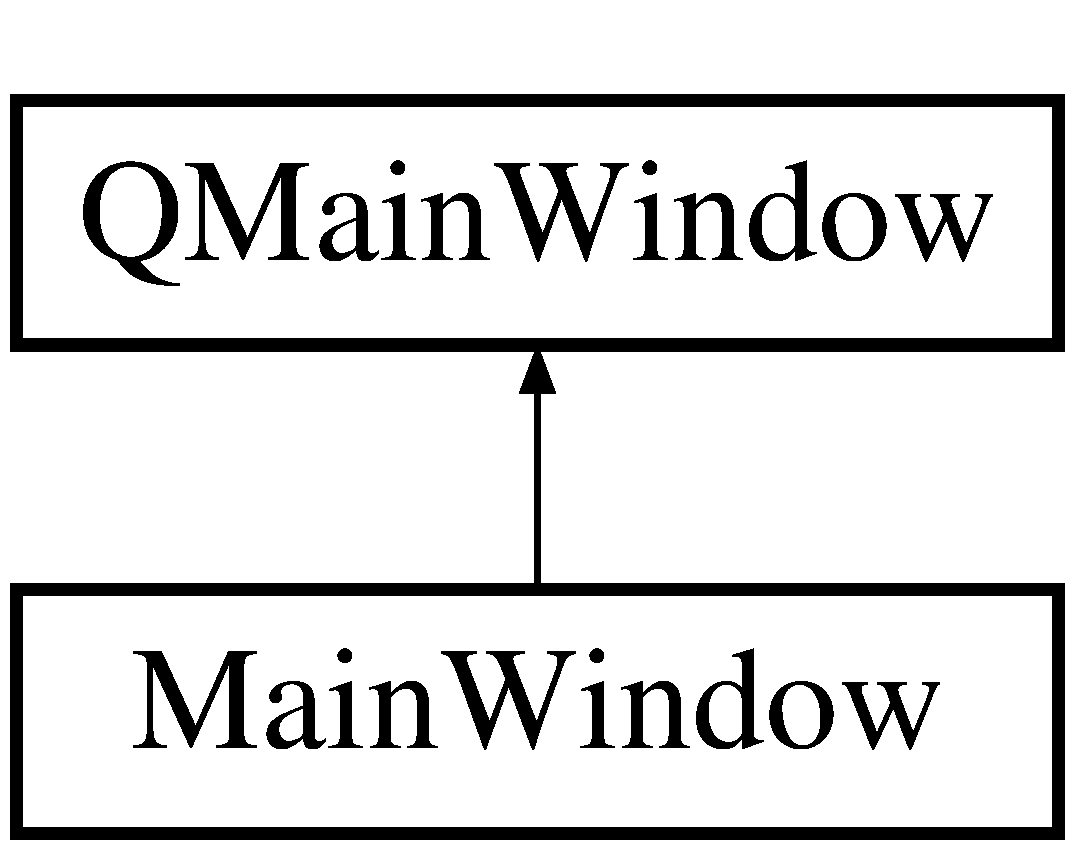
\includegraphics[height=2.000000cm]{class_main_window}
\end{center}
\end{figure}
\subsection*{Public Member Functions}
\begin{DoxyCompactItemize}
\item 
\hyperlink{class_main_window_a8b244be8b7b7db1b08de2a2acb9409db}{Main\+Window} (Q\+Widget $\ast$parent=0)
\item 
void \hyperlink{class_main_window_adc0662d3cc64fcb561bfd6ac8b09726c}{populate\+Conference\+Drop\+Down\+Box} (Q\+String box)
\item 
\mbox{\Hypertarget{class_main_window_a281137be7e79828fe96c4959c8b9ebe6}\label{class_main_window_a281137be7e79828fe96c4959c8b9ebe6}} 
void {\bfseries populate\+Trip\+Selection\+Drop\+Down\+Box} ()
\item 
\mbox{\Hypertarget{class_main_window_a54af06c29e75a4fe491e006a20d9d90b}\label{class_main_window_a54af06c29e75a4fe491e006a20d9d90b}} 
void {\bfseries populate\+Dijkstras\+Drop\+Down\+Box} ()
\item 
\mbox{\Hypertarget{class_main_window_a355c912d60d63c0c076658def96e6201}\label{class_main_window_a355c912d60d63c0c076658def96e6201}} 
void {\bfseries populate\+D\+F\+Sand\+B\+F\+Sdrop\+Down\+Box} ()
\item 
\mbox{\Hypertarget{class_main_window_a505a2178bd2176455f98b784b328d3bf}\label{class_main_window_a505a2178bd2176455f98b784b328d3bf}} 
void {\bfseries show\+Starting\+Trip\+Inputs} ()
\item 
\mbox{\Hypertarget{class_main_window_accf97cf25e538c019e1fe48910e35c95}\label{class_main_window_accf97cf25e538c019e1fe48910e35c95}} 
void {\bfseries visit\+All\+Stadiums\+Efficiently} (Q\+String starting\+Stadium, Q\+String\+List stadiums\+To\+Visit, Q\+Vector$<$ Q\+String $>$ \&visited\+Stadiums)
\item 
\mbox{\Hypertarget{class_main_window_a72dc5e4404b2966dc03a3694a9cdfd21}\label{class_main_window_a72dc5e4404b2966dc03a3694a9cdfd21}} 
void {\bfseries hide\+Secondary\+Trip\+Inputs} ()
\item 
\mbox{\Hypertarget{class_main_window_a77dac0add3c158454ce4b8b6e8579008}\label{class_main_window_a77dac0add3c158454ce4b8b6e8579008}} 
void {\bfseries dream\+Vacation} (Q\+String start\+Stadium, Q\+String\+List trip\+List, Q\+String\+List \&visited\+Stadiums)
\end{DoxyCompactItemize}
\subsection*{Private Slots}
\begin{DoxyCompactItemize}
\item 
void \hyperlink{class_main_window_a009f72c029e675a368a4dd3aad2d52f6}{on\+\_\+\+A\+F\+L\+Check\+Box\+\_\+clicked} ()
\item 
void \hyperlink{class_main_window_ab17eb6df3cc6031458d0d0fe139f2de5}{on\+\_\+\+N\+F\+L\+Check\+Box\+\_\+clicked} ()
\item 
void \hyperlink{class_main_window_a042e8c2a44f0917066a389d93afd3c7a}{on\+\_\+\+Both\+Check\+Box\+\_\+clicked} ()
\item 
void \hyperlink{class_main_window_a6b44c6e98ed39eb1a633c93c60f34e6f}{on\+\_\+\+Teams\+Combo\+Box\+\_\+current\+Index\+Changed} (const Q\+String \&arg1)
\item 
\mbox{\Hypertarget{class_main_window_ac447cca664d027a25bb0d132752718a0}\label{class_main_window_ac447cca664d027a25bb0d132752718a0}} 
void {\bfseries on\+\_\+admin\+Button\+\_\+clicked} ()
\item 
void \hyperlink{class_main_window_aff2bf52ba8193c96f87e98359fe39041}{on\+\_\+roof\+Combo\+Box\+\_\+current\+Index\+Changed} (const Q\+String \&arg1)
\begin{DoxyCompactList}\small\item\em on\+\_\+combo\+Box\+\_\+current\+Index\+Changed \end{DoxyCompactList}\item 
\mbox{\Hypertarget{class_main_window_a738c75b6db1208e2378a539403c6aff9}\label{class_main_window_a738c75b6db1208e2378a539403c6aff9}} 
void {\bfseries on\+\_\+tab\+Widget\+\_\+tab\+Bar\+Clicked} (int index)
\item 
\mbox{\Hypertarget{class_main_window_ab3e92d8bc5acf84fb75615a5e379f90a}\label{class_main_window_ab3e92d8bc5acf84fb75615a5e379f90a}} 
void {\bfseries on\+\_\+add\+To\+Trip\+Button\+\_\+clicked} ()
\item 
\mbox{\Hypertarget{class_main_window_afa7470de361f56ec45d9e8e5630fb46e}\label{class_main_window_afa7470de361f56ec45d9e8e5630fb46e}} 
void {\bfseries on\+\_\+trip\+Creation\+Combo\+Box\+\_\+current\+Index\+Changed} (int index)
\item 
\mbox{\Hypertarget{class_main_window_a035f2eb137759b311f9cfe067ccc46d8}\label{class_main_window_a035f2eb137759b311f9cfe067ccc46d8}} 
void {\bfseries on\+\_\+finish\+Adding\+Button\+\_\+clicked} ()
\item 
\mbox{\Hypertarget{class_main_window_a1b0a71532f0f5e71a92907ecc66276ba}\label{class_main_window_a1b0a71532f0f5e71a92907ecc66276ba}} 
void {\bfseries on\+\_\+start\+Trip\+Button\+\_\+clicked} ()
\item 
\mbox{\Hypertarget{class_main_window_a04ec468348571e9dd5c3cdc0a34cd590}\label{class_main_window_a04ec468348571e9dd5c3cdc0a34cd590}} 
void {\bfseries on\+\_\+next\+College\+Button\+\_\+clicked} ()
\item 
\mbox{\Hypertarget{class_main_window_a48febb3456f23f978d69b6d1a0bd1676}\label{class_main_window_a48febb3456f23f978d69b6d1a0bd1676}} 
void {\bfseries on\+\_\+starting\+Stadium\+Combo\+Box\+Dijkstras\+\_\+current\+Index\+Changed} (const Q\+String \&arg1)
\item 
\mbox{\Hypertarget{class_main_window_a8b38dc73a7ab40d56befb134d276e467}\label{class_main_window_a8b38dc73a7ab40d56befb134d276e467}} 
void {\bfseries on\+\_\+ending\+Stadium\+Combo\+Box\+Dijkstras\+\_\+current\+Index\+Changed} (const Q\+String \&arg1)
\item 
\mbox{\Hypertarget{class_main_window_a4e0e0ec958fcabd367a5094389b8d380}\label{class_main_window_a4e0e0ec958fcabd367a5094389b8d380}} 
void {\bfseries on\+\_\+visit\+All\+Stadiums\+Button\+\_\+clicked} ()
\item 
\mbox{\Hypertarget{class_main_window_ad78a32b3aa8fae318e326a8a0f1ab9f5}\label{class_main_window_ad78a32b3aa8fae318e326a8a0f1ab9f5}} 
void {\bfseries on\+\_\+reset\+Trip\+Button\+\_\+clicked} ()
\item 
\mbox{\Hypertarget{class_main_window_a78217438ec4b04b221c04a7b3d908469}\label{class_main_window_a78217438ec4b04b221c04a7b3d908469}} 
void {\bfseries on\+\_\+\+B\+F\+Sstart\+Button\+\_\+clicked} ()
\item 
\mbox{\Hypertarget{class_main_window_ab5ec4a06e4e38781eb7b913fed92733e}\label{class_main_window_ab5ec4a06e4e38781eb7b913fed92733e}} 
void {\bfseries on\+\_\+tab\+Widget\+\_\+current\+Changed} (int index)
\item 
\mbox{\Hypertarget{class_main_window_ab563c0d9e0225b55585cbfdba998c3cc}\label{class_main_window_ab563c0d9e0225b55585cbfdba998c3cc}} 
void {\bfseries on\+\_\+spin\+Box\+\_\+value\+Changed} (int arg1)
\item 
\mbox{\Hypertarget{class_main_window_a1ca615293b8c2dbeef99dbf61e82bb55}\label{class_main_window_a1ca615293b8c2dbeef99dbf61e82bb55}} 
void {\bfseries on\+\_\+souvenir\+Table\+\_\+clicked} (const Q\+Model\+Index \&index)
\item 
\mbox{\Hypertarget{class_main_window_a1a7f2c3750064fcfc2af7b82e6e1f649}\label{class_main_window_a1a7f2c3750064fcfc2af7b82e6e1f649}} 
void {\bfseries on\+\_\+purchase\+Button\+\_\+clicked} ()
\item 
\mbox{\Hypertarget{class_main_window_aea2558859c02d5d8526863c8d3a1c272}\label{class_main_window_aea2558859c02d5d8526863c8d3a1c272}} 
void {\bfseries on\+\_\+dream\+Vacation\+Button\+\_\+clicked} ()
\item 
\mbox{\Hypertarget{class_main_window_a1d1b4ddc9165c7c0b8b4621cca3318a0}\label{class_main_window_a1d1b4ddc9165c7c0b8b4621cca3318a0}} 
void {\bfseries on\+\_\+\+M\+S\+T\+Button\+\_\+clicked} ()
\end{DoxyCompactItemize}
\subsection*{Private Attributes}
\begin{DoxyCompactItemize}
\item 
\mbox{\Hypertarget{class_main_window_a35466a70ed47252a0191168126a352a5}\label{class_main_window_a35466a70ed47252a0191168126a352a5}} 
\hyperlink{class_ui_1_1_main_window}{Ui\+::\+Main\+Window} $\ast$ {\bfseries ui}
\item 
\mbox{\Hypertarget{class_main_window_a86bf1caf2fb7f33313c6666c9621f2bb}\label{class_main_window_a86bf1caf2fb7f33313c6666c9621f2bb}} 
\hyperlink{classadmin_window}{admin\+Window} $\ast$ {\bfseries admin}
\item 
\mbox{\Hypertarget{class_main_window_a14e45697dcf41d51d7c7b897115f37ec}\label{class_main_window_a14e45697dcf41d51d7c7b897115f37ec}} 
int {\bfseries trip\+Table\+View\+Row\+Number}
\item 
\mbox{\Hypertarget{class_main_window_aaa04d341765d51fa0fa21099b3332151}\label{class_main_window_aaa04d341765d51fa0fa21099b3332151}} 
int {\bfseries B\+F\+Stable\+Widgit\+Row\+Number}
\item 
\mbox{\Hypertarget{class_main_window_ab404f01fde474411e4db9f48a597933b}\label{class_main_window_ab404f01fde474411e4db9f48a597933b}} 
Q\+Standard\+Item\+Model $\ast$ {\bfseries table}
\item 
\mbox{\Hypertarget{class_main_window_a455b66a7c7955b81e4413b2de6ed365f}\label{class_main_window_a455b66a7c7955b81e4413b2de6ed365f}} 
Q\+Standard\+Item\+Model $\ast$ {\bfseries B\+F\+Swidgit}
\item 
\mbox{\Hypertarget{class_main_window_a64858232db731ca5b8176f44c3d8449b}\label{class_main_window_a64858232db731ca5b8176f44c3d8449b}} 
Q\+Vector$<$ \hyperlink{structcollege_stadium_pair}{college\+Stadium\+Pair} $>$ {\bfseries stadium\+Trip}
\item 
\mbox{\Hypertarget{class_main_window_af80069d0c00ad7e1c9ad338679176617}\label{class_main_window_af80069d0c00ad7e1c9ad338679176617}} 
int {\bfseries current\+Stadium\+Index}
\item 
\mbox{\Hypertarget{class_main_window_a26b6b2c19d6ed3714dd32945e86fff4c}\label{class_main_window_a26b6b2c19d6ed3714dd32945e86fff4c}} 
\hyperlink{class_cart}{Cart} $\ast$ {\bfseries purchases}
\item 
\mbox{\Hypertarget{class_main_window_a4b44a975e1f8ead51f450c55bbcea363}\label{class_main_window_a4b44a975e1f8ead51f450c55bbcea363}} 
\hyperlink{class_map}{Map} {\bfseries Souvenirs}
\item 
\mbox{\Hypertarget{class_main_window_a593e58f15e10145314c4e7c401c16551}\label{class_main_window_a593e58f15e10145314c4e7c401c16551}} 
int {\bfseries total\+Distance}
\item 
\mbox{\Hypertarget{class_main_window_ad9ea6e0dda2bf786ee14e6e21543340f}\label{class_main_window_ad9ea6e0dda2bf786ee14e6e21543340f}} 
Q\+String\+List {\bfseries list\+Trip}
\item 
\mbox{\Hypertarget{class_main_window_a2f0480846829d065d908b5f3bfaac814}\label{class_main_window_a2f0480846829d065d908b5f3bfaac814}} 
\hyperlink{class_graph}{Graph} {\bfseries stadium\+Map}
\item 
\mbox{\Hypertarget{class_main_window_ad7ca6ae1c5740a3f4d36209d05d74a4e}\label{class_main_window_ad7ca6ae1c5740a3f4d36209d05d74a4e}} 
Q\+Model\+Index {\bfseries souvenir\+Index}
\item 
\mbox{\Hypertarget{class_main_window_a37988a42ba9e5ead55cf604a7e8fef20}\label{class_main_window_a37988a42ba9e5ead55cf604a7e8fef20}} 
int {\bfseries souvenir\+Quantity}
\item 
\mbox{\Hypertarget{class_main_window_a2876abf41a986132407eb7e62e915088}\label{class_main_window_a2876abf41a986132407eb7e62e915088}} 
int {\bfseries total\+Amount\+Row\+Index}
\item 
\mbox{\Hypertarget{class_main_window_a3a98197e57eba8cbbe9c310d0a6f7838}\label{class_main_window_a3a98197e57eba8cbbe9c310d0a6f7838}} 
bool {\bfseries souvenir\+Selected}
\end{DoxyCompactItemize}


\subsection{Constructor \& Destructor Documentation}
\mbox{\Hypertarget{class_main_window_a8b244be8b7b7db1b08de2a2acb9409db}\label{class_main_window_a8b244be8b7b7db1b08de2a2acb9409db}} 
\index{Main\+Window@{Main\+Window}!Main\+Window@{Main\+Window}}
\index{Main\+Window@{Main\+Window}!Main\+Window@{Main\+Window}}
\subsubsection{\texorpdfstring{Main\+Window()}{MainWindow()}}
{\footnotesize\ttfamily Main\+Window\+::\+Main\+Window (\begin{DoxyParamCaption}\item[{Q\+Widget $\ast$}]{parent = {\ttfamily 0} }\end{DoxyParamCaption})\hspace{0.3cm}{\ttfamily [explicit]}}


\begin{DoxyParams}{Parameters}
{\em parent} & \\
\hline
\end{DoxyParams}


\subsection{Member Function Documentation}
\mbox{\Hypertarget{class_main_window_a009f72c029e675a368a4dd3aad2d52f6}\label{class_main_window_a009f72c029e675a368a4dd3aad2d52f6}} 
\index{Main\+Window@{Main\+Window}!on\+\_\+\+A\+F\+L\+Check\+Box\+\_\+clicked@{on\+\_\+\+A\+F\+L\+Check\+Box\+\_\+clicked}}
\index{on\+\_\+\+A\+F\+L\+Check\+Box\+\_\+clicked@{on\+\_\+\+A\+F\+L\+Check\+Box\+\_\+clicked}!Main\+Window@{Main\+Window}}
\subsubsection{\texorpdfstring{on\+\_\+\+A\+F\+L\+Check\+Box\+\_\+clicked}{on\_AFLCheckBox\_clicked}}
{\footnotesize\ttfamily void Main\+Window\+::on\+\_\+\+A\+F\+L\+Check\+Box\+\_\+clicked (\begin{DoxyParamCaption}{ }\end{DoxyParamCaption})\hspace{0.3cm}{\ttfamily [private]}, {\ttfamily [slot]}}

allows the table to be sorted by clicking on the header \mbox{\Hypertarget{class_main_window_a042e8c2a44f0917066a389d93afd3c7a}\label{class_main_window_a042e8c2a44f0917066a389d93afd3c7a}} 
\index{Main\+Window@{Main\+Window}!on\+\_\+\+Both\+Check\+Box\+\_\+clicked@{on\+\_\+\+Both\+Check\+Box\+\_\+clicked}}
\index{on\+\_\+\+Both\+Check\+Box\+\_\+clicked@{on\+\_\+\+Both\+Check\+Box\+\_\+clicked}!Main\+Window@{Main\+Window}}
\subsubsection{\texorpdfstring{on\+\_\+\+Both\+Check\+Box\+\_\+clicked}{on\_BothCheckBox\_clicked}}
{\footnotesize\ttfamily void Main\+Window\+::on\+\_\+\+Both\+Check\+Box\+\_\+clicked (\begin{DoxyParamCaption}{ }\end{DoxyParamCaption})\hspace{0.3cm}{\ttfamily [private]}, {\ttfamily [slot]}}

allows the table to be sorted by clicking on the header \mbox{\Hypertarget{class_main_window_ab17eb6df3cc6031458d0d0fe139f2de5}\label{class_main_window_ab17eb6df3cc6031458d0d0fe139f2de5}} 
\index{Main\+Window@{Main\+Window}!on\+\_\+\+N\+F\+L\+Check\+Box\+\_\+clicked@{on\+\_\+\+N\+F\+L\+Check\+Box\+\_\+clicked}}
\index{on\+\_\+\+N\+F\+L\+Check\+Box\+\_\+clicked@{on\+\_\+\+N\+F\+L\+Check\+Box\+\_\+clicked}!Main\+Window@{Main\+Window}}
\subsubsection{\texorpdfstring{on\+\_\+\+N\+F\+L\+Check\+Box\+\_\+clicked}{on\_NFLCheckBox\_clicked}}
{\footnotesize\ttfamily void Main\+Window\+::on\+\_\+\+N\+F\+L\+Check\+Box\+\_\+clicked (\begin{DoxyParamCaption}{ }\end{DoxyParamCaption})\hspace{0.3cm}{\ttfamily [private]}, {\ttfamily [slot]}}

allows the table to be sorted by clicking on the header \mbox{\Hypertarget{class_main_window_aff2bf52ba8193c96f87e98359fe39041}\label{class_main_window_aff2bf52ba8193c96f87e98359fe39041}} 
\index{Main\+Window@{Main\+Window}!on\+\_\+roof\+Combo\+Box\+\_\+current\+Index\+Changed@{on\+\_\+roof\+Combo\+Box\+\_\+current\+Index\+Changed}}
\index{on\+\_\+roof\+Combo\+Box\+\_\+current\+Index\+Changed@{on\+\_\+roof\+Combo\+Box\+\_\+current\+Index\+Changed}!Main\+Window@{Main\+Window}}
\subsubsection{\texorpdfstring{on\+\_\+roof\+Combo\+Box\+\_\+current\+Index\+Changed}{on\_roofComboBox\_currentIndexChanged}}
{\footnotesize\ttfamily void Main\+Window\+::on\+\_\+roof\+Combo\+Box\+\_\+current\+Index\+Changed (\begin{DoxyParamCaption}\item[{const Q\+String \&}]{arg1 }\end{DoxyParamCaption})\hspace{0.3cm}{\ttfamily [private]}, {\ttfamily [slot]}}



on\+\_\+combo\+Box\+\_\+current\+Index\+Changed 

allows the table to be sorted by clicking on the header \mbox{\Hypertarget{class_main_window_a6b44c6e98ed39eb1a633c93c60f34e6f}\label{class_main_window_a6b44c6e98ed39eb1a633c93c60f34e6f}} 
\index{Main\+Window@{Main\+Window}!on\+\_\+\+Teams\+Combo\+Box\+\_\+current\+Index\+Changed@{on\+\_\+\+Teams\+Combo\+Box\+\_\+current\+Index\+Changed}}
\index{on\+\_\+\+Teams\+Combo\+Box\+\_\+current\+Index\+Changed@{on\+\_\+\+Teams\+Combo\+Box\+\_\+current\+Index\+Changed}!Main\+Window@{Main\+Window}}
\subsubsection{\texorpdfstring{on\+\_\+\+Teams\+Combo\+Box\+\_\+current\+Index\+Changed}{on\_TeamsComboBox\_currentIndexChanged}}
{\footnotesize\ttfamily void Main\+Window\+::on\+\_\+\+Teams\+Combo\+Box\+\_\+current\+Index\+Changed (\begin{DoxyParamCaption}\item[{const Q\+String \&}]{arg1 }\end{DoxyParamCaption})\hspace{0.3cm}{\ttfamily [private]}, {\ttfamily [slot]}}


\begin{DoxyParams}{Parameters}
{\em arg1} & \\
\hline
\end{DoxyParams}
allows the table to be sorted by clicking on the header \mbox{\Hypertarget{class_main_window_adc0662d3cc64fcb561bfd6ac8b09726c}\label{class_main_window_adc0662d3cc64fcb561bfd6ac8b09726c}} 
\index{Main\+Window@{Main\+Window}!populate\+Conference\+Drop\+Down\+Box@{populate\+Conference\+Drop\+Down\+Box}}
\index{populate\+Conference\+Drop\+Down\+Box@{populate\+Conference\+Drop\+Down\+Box}!Main\+Window@{Main\+Window}}
\subsubsection{\texorpdfstring{populate\+Conference\+Drop\+Down\+Box()}{populateConferenceDropDownBox()}}
{\footnotesize\ttfamily void Main\+Window\+::populate\+Conference\+Drop\+Down\+Box (\begin{DoxyParamCaption}\item[{Q\+String}]{box }\end{DoxyParamCaption})}


\begin{DoxyParams}{Parameters}
{\em box} & \\
\hline
\end{DoxyParams}
If option is A\+FL

If option is N\+FL

If option is both A\+FL and N\+FL 

The documentation for this class was generated from the following files\+:\begin{DoxyCompactItemize}
\item 
mainwindow.\+h\item 
mainwindow.\+cpp\end{DoxyCompactItemize}

\hypertarget{class_ui_1_1_main_window}{}\section{Ui\+:\+:Main\+Window Class Reference}
\label{class_ui_1_1_main_window}\index{Ui\+::\+Main\+Window@{Ui\+::\+Main\+Window}}
Inheritance diagram for Ui\+:\+:Main\+Window\+:\begin{figure}[H]
\begin{center}
\leavevmode
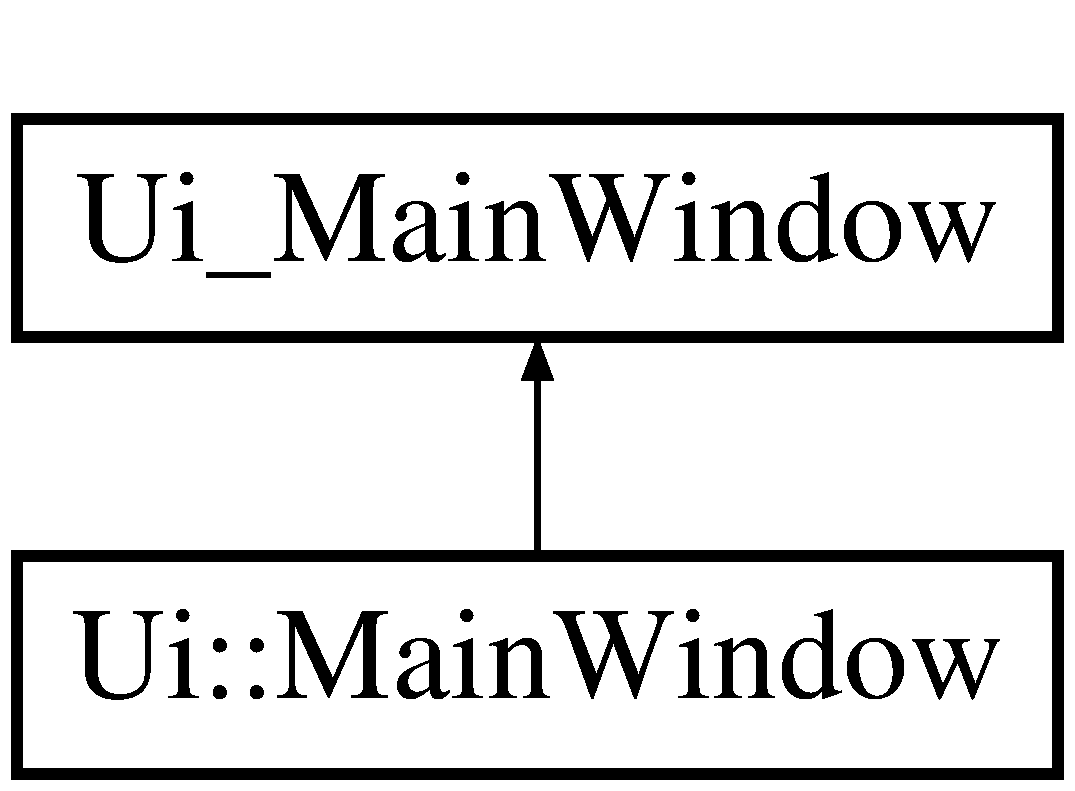
\includegraphics[height=2.000000cm]{class_ui_1_1_main_window}
\end{center}
\end{figure}
\subsection*{Additional Inherited Members}


The documentation for this class was generated from the following file\+:\begin{DoxyCompactItemize}
\item 
ui\+\_\+mainwindow.\+h\end{DoxyCompactItemize}

\hypertarget{class_map}{}\section{Map Class Reference}
\label{class_map}\index{Map@{Map}}
\subsection*{Public Member Functions}
\begin{DoxyCompactItemize}
\item 
\mbox{\Hypertarget{class_map_a74002e2be89c3eae7f045db1666933a2}\label{class_map_a74002e2be89c3eae7f045db1666933a2}} 
{\bfseries Map} (int capacity)
\item 
\mbox{\Hypertarget{class_map_a34e3e168f646953aed049c0bf37fb62b}\label{class_map_a34e3e168f646953aed049c0bf37fb62b}} 
void {\bfseries set\+Capacity} (int capacity)
\item 
\mbox{\Hypertarget{class_map_aef091383ecb1bd251ca304eafd5c462f}\label{class_map_aef091383ecb1bd251ca304eafd5c462f}} 
void {\bfseries put} (\hyperlink{class_map_node}{Map\+Node}, Q\+String)
\item 
\mbox{\Hypertarget{class_map_a9c6dc88a70dcf25e3371d8bc4ec35ad0}\label{class_map_a9c6dc88a70dcf25e3371d8bc4ec35ad0}} 
void {\bfseries print} ()
\item 
\mbox{\Hypertarget{class_map_a8cfc8e8ee3a77497b8e6a2fc4cde6e5e}\label{class_map_a8cfc8e8ee3a77497b8e6a2fc4cde6e5e}} 
void {\bfseries remove} (Q\+String key, Q\+String souvenir\+Name)
\end{DoxyCompactItemize}
\subsection*{Private Member Functions}
\begin{DoxyCompactItemize}
\item 
\mbox{\Hypertarget{class_map_a79cd7cd192742d3c40a799c8d97692a7}\label{class_map_a79cd7cd192742d3c40a799c8d97692a7}} 
int {\bfseries get\+Valid\+Index} (Q\+String key, int j, int k)
\item 
\mbox{\Hypertarget{class_map_a99a3d48266107311800c37510990fa09}\label{class_map_a99a3d48266107311800c37510990fa09}} 
int {\bfseries translate\+Key\+Into\+Int} (Q\+String key)
\item 
\mbox{\Hypertarget{class_map_adb144638ae9aa7abed9a382eb1c9176b}\label{class_map_adb144638ae9aa7abed9a382eb1c9176b}} 
int {\bfseries get\+Valid\+Index} (Q\+String key)
\item 
\mbox{\Hypertarget{class_map_aea2092236b97fa1f8c5bce8b904f74ea}\label{class_map_aea2092236b97fa1f8c5bce8b904f74ea}} 
int {\bfseries equation\+One} (int key)
\item 
\mbox{\Hypertarget{class_map_a12437a11e54a0f03abb3625c80598eca}\label{class_map_a12437a11e54a0f03abb3625c80598eca}} 
int {\bfseries equation\+Two} (int key)
\item 
\mbox{\Hypertarget{class_map_a5d72dbf2a778e81d4cf4a48a3eb2a427}\label{class_map_a5d72dbf2a778e81d4cf4a48a3eb2a427}} 
int {\bfseries find} (Q\+String key)
\item 
\mbox{\Hypertarget{class_map_a6c3368c129c15e03cd38d5308ca919ae}\label{class_map_a6c3368c129c15e03cd38d5308ca919ae}} 
int {\bfseries find} (Q\+String key, int j)
\end{DoxyCompactItemize}
\subsection*{Private Attributes}
\begin{DoxyCompactItemize}
\item 
\mbox{\Hypertarget{class_map_a60146aa4b52ce279c71ab2d454713ba8}\label{class_map_a60146aa4b52ce279c71ab2d454713ba8}} 
\hyperlink{class_map_node}{Map\+Node} $\ast$ {\bfseries ar}
\item 
\mbox{\Hypertarget{class_map_a5317a76ed7e281b2b9dd6726e2e836a9}\label{class_map_a5317a76ed7e281b2b9dd6726e2e836a9}} 
int {\bfseries capacity}
\end{DoxyCompactItemize}


The documentation for this class was generated from the following files\+:\begin{DoxyCompactItemize}
\item 
map.\+h\item 
map.\+cpp\end{DoxyCompactItemize}

\hypertarget{class_map_node}{}\section{Map\+Node Class Reference}
\label{class_map_node}\index{Map\+Node@{Map\+Node}}
\subsection*{Public Member Functions}
\begin{DoxyCompactItemize}
\item 
\mbox{\Hypertarget{class_map_node_ab17429369aa016758d8019cb6d711f89}\label{class_map_node_ab17429369aa016758d8019cb6d711f89}} 
{\bfseries Map\+Node} (Q\+String value)
\item 
\mbox{\Hypertarget{class_map_node_a37c08b0ef2914ee3192cf8b4ced0a73c}\label{class_map_node_a37c08b0ef2914ee3192cf8b4ced0a73c}} 
Q\+String {\bfseries get\+Value} () const
\item 
\mbox{\Hypertarget{class_map_node_a8e0e044b760aa71c6e8ab4b437d00bc2}\label{class_map_node_a8e0e044b760aa71c6e8ab4b437d00bc2}} 
void {\bfseries set\+Value} (Q\+String val)
\item 
\mbox{\Hypertarget{class_map_node_af3732a07deb8c0c2479dc692c7dc5925}\label{class_map_node_af3732a07deb8c0c2479dc692c7dc5925}} 
void {\bfseries set\+Key} (Q\+String k)
\item 
\mbox{\Hypertarget{class_map_node_a89e08f984169029557f0a1d55c9589a0}\label{class_map_node_a89e08f984169029557f0a1d55c9589a0}} 
Q\+String {\bfseries get\+Key} () const
\item 
\mbox{\Hypertarget{class_map_node_a38667f219cc961d05f1b1dbe992f6419}\label{class_map_node_a38667f219cc961d05f1b1dbe992f6419}} 
bool {\bfseries is\+Occupied} ()
\item 
\mbox{\Hypertarget{class_map_node_a0b540119ef1bb56b08a7e78b18423d81}\label{class_map_node_a0b540119ef1bb56b08a7e78b18423d81}} 
void {\bfseries set\+Available} ()
\item 
\mbox{\Hypertarget{class_map_node_a18d7e869ab2b41b195468a51f773ed74}\label{class_map_node_a18d7e869ab2b41b195468a51f773ed74}} 
void {\bfseries add\+Souvenir} (\hyperlink{class_souvenir}{Souvenir} s)
\item 
\mbox{\Hypertarget{class_map_node_a93399ff797254eb384d3980d9703fd14}\label{class_map_node_a93399ff797254eb384d3980d9703fd14}} 
\hyperlink{class_map_node}{Map\+Node} {\bfseries operator=} (const \hyperlink{class_map_node}{Map\+Node} \&arg)
\item 
\mbox{\Hypertarget{class_map_node_a5b944284ebea6e3d2fe12f6703ad20d6}\label{class_map_node_a5b944284ebea6e3d2fe12f6703ad20d6}} 
Q\+Vector$<$ \hyperlink{class_souvenir}{Souvenir} $>$ {\bfseries get\+Souvenirs} ()
\end{DoxyCompactItemize}
\subsection*{Private Attributes}
\begin{DoxyCompactItemize}
\item 
\mbox{\Hypertarget{class_map_node_a96c7b1b1fabcce7d5711f8b02ae01197}\label{class_map_node_a96c7b1b1fabcce7d5711f8b02ae01197}} 
Q\+String {\bfseries value}
\item 
\mbox{\Hypertarget{class_map_node_a1868cacdc70ce21145990e7f76826c7e}\label{class_map_node_a1868cacdc70ce21145990e7f76826c7e}} 
Q\+Vector$<$ \hyperlink{class_souvenir}{Souvenir} $>$ {\bfseries souvenirs}
\item 
\mbox{\Hypertarget{class_map_node_a8b2e1229b3d58503d84758fa0fbb61be}\label{class_map_node_a8b2e1229b3d58503d84758fa0fbb61be}} 
Q\+String {\bfseries key}
\item 
\mbox{\Hypertarget{class_map_node_aad4e757ae63dce3f8ddccbf9d2892cdd}\label{class_map_node_aad4e757ae63dce3f8ddccbf9d2892cdd}} 
bool {\bfseries occupied}
\end{DoxyCompactItemize}


The documentation for this class was generated from the following files\+:\begin{DoxyCompactItemize}
\item 
mapnode.\+h\item 
mapnode.\+cpp\end{DoxyCompactItemize}

\hypertarget{class_ui_1_1modifysouvenirs}{}\section{Ui\+:\+:modifysouvenirs Class Reference}
\label{class_ui_1_1modifysouvenirs}\index{Ui\+::modifysouvenirs@{Ui\+::modifysouvenirs}}


Inheritance diagram for Ui\+:\+:modifysouvenirs\+:\nopagebreak
\begin{figure}[H]
\begin{center}
\leavevmode
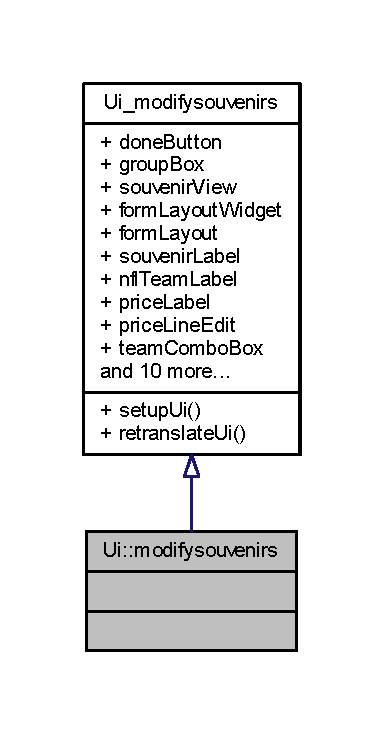
\includegraphics[width=184pt]{class_ui_1_1modifysouvenirs__inherit__graph}
\end{center}
\end{figure}


Collaboration diagram for Ui\+:\+:modifysouvenirs\+:\nopagebreak
\begin{figure}[H]
\begin{center}
\leavevmode
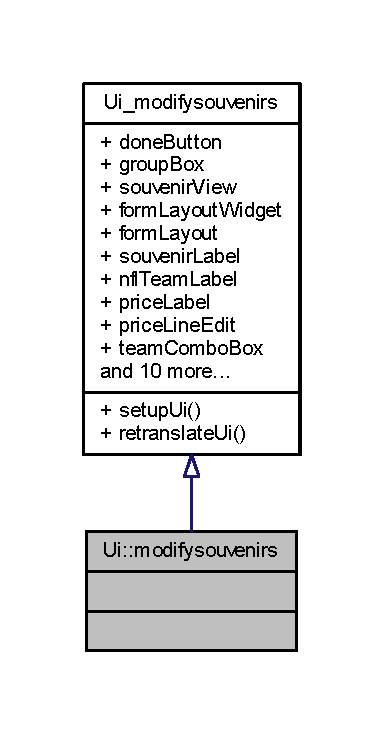
\includegraphics[width=184pt]{class_ui_1_1modifysouvenirs__coll__graph}
\end{center}
\end{figure}
\subsection*{Additional Inherited Members}


The documentation for this class was generated from the following file\+:\begin{DoxyCompactItemize}
\item 
ui\+\_\+modifysouvenirs.\+h\end{DoxyCompactItemize}

\hypertarget{classmodifysouvenirs}{}\section{modifysouvenirs Class Reference}
\label{classmodifysouvenirs}\index{modifysouvenirs@{modifysouvenirs}}
Inheritance diagram for modifysouvenirs\+:\begin{figure}[H]
\begin{center}
\leavevmode
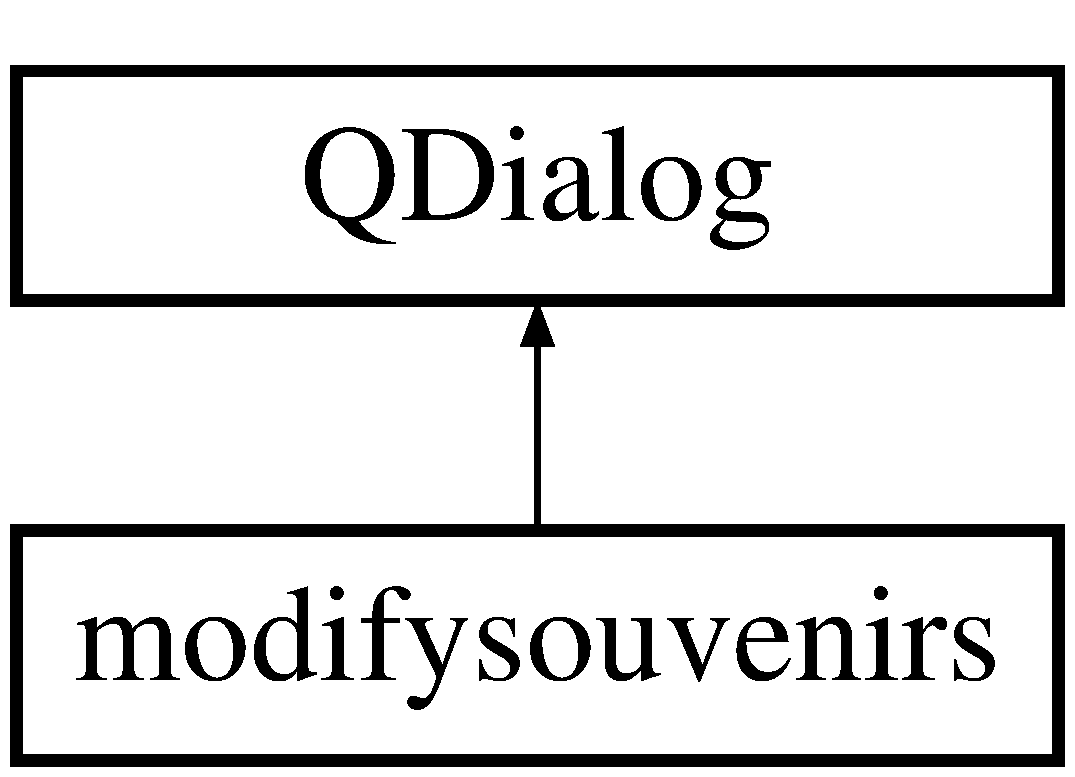
\includegraphics[height=2.000000cm]{classmodifysouvenirs}
\end{center}
\end{figure}
\subsection*{Public Member Functions}
\begin{DoxyCompactItemize}
\item 
\mbox{\Hypertarget{classmodifysouvenirs_ae8cf83ce05a01274522a341a8e081928}\label{classmodifysouvenirs_ae8cf83ce05a01274522a341a8e081928}} 
{\bfseries modifysouvenirs} (Q\+Widget $\ast$parent=0)
\item 
\mbox{\Hypertarget{classmodifysouvenirs_ad15ff72e8ed3361501972a0927f687ab}\label{classmodifysouvenirs_ad15ff72e8ed3361501972a0927f687ab}} 
void {\bfseries set\+Graph\+Pointer} (\hyperlink{class_graph}{Graph} $\ast$p)
\end{DoxyCompactItemize}
\subsection*{Private Slots}
\begin{DoxyCompactItemize}
\item 
\mbox{\Hypertarget{classmodifysouvenirs_ab06c14688d7494cb7ce9cf2fbe44af28}\label{classmodifysouvenirs_ab06c14688d7494cb7ce9cf2fbe44af28}} 
void {\bfseries on\+\_\+add\+Souvenir\+\_\+clicked} ()
\item 
\mbox{\Hypertarget{classmodifysouvenirs_ace1bd0c05652f2d229f927db537a8d34}\label{classmodifysouvenirs_ace1bd0c05652f2d229f927db537a8d34}} 
void {\bfseries on\+\_\+delete\+Souvenir\+\_\+clicked} ()
\item 
\mbox{\Hypertarget{classmodifysouvenirs_a519bd0776e2e27409672cfe8ec01c028}\label{classmodifysouvenirs_a519bd0776e2e27409672cfe8ec01c028}} 
void {\bfseries on\+\_\+modify\+Souvenir\+\_\+clicked} ()
\item 
\mbox{\Hypertarget{classmodifysouvenirs_af634b7e0b13202888e488eca427dcbe3}\label{classmodifysouvenirs_af634b7e0b13202888e488eca427dcbe3}} 
void {\bfseries on\+\_\+done\+Button\+\_\+clicked} ()
\item 
\mbox{\Hypertarget{classmodifysouvenirs_acf60b19ef0276764bc649d0cfb641a60}\label{classmodifysouvenirs_acf60b19ef0276764bc649d0cfb641a60}} 
void {\bfseries on\+\_\+add\+Sandiego\+Sailors\+Button\+\_\+clicked} ()
\item 
\mbox{\Hypertarget{classmodifysouvenirs_afdce02d3ffbbd2f00cbb100816ec831e}\label{classmodifysouvenirs_afdce02d3ffbbd2f00cbb100816ec831e}} 
void {\bfseries on\+\_\+team\+Combo\+Box\+\_\+current\+Index\+Changed} (const Q\+String \&arg1)
\item 
\mbox{\Hypertarget{classmodifysouvenirs_a70369cade8961963f7e98d59dea124df}\label{classmodifysouvenirs_a70369cade8961963f7e98d59dea124df}} 
void {\bfseries update\+Souvenir\+View} ()
\end{DoxyCompactItemize}
\subsection*{Private Attributes}
\begin{DoxyCompactItemize}
\item 
\mbox{\Hypertarget{classmodifysouvenirs_a91d4c3a315d423d8c0493bb16b298967}\label{classmodifysouvenirs_a91d4c3a315d423d8c0493bb16b298967}} 
\hyperlink{class_ui_1_1modifysouvenirs}{Ui\+::modifysouvenirs} $\ast$ {\bfseries ui}
\item 
\mbox{\Hypertarget{classmodifysouvenirs_af69425e84f9683db36153e2b97ec5313}\label{classmodifysouvenirs_af69425e84f9683db36153e2b97ec5313}} 
\hyperlink{class_graph}{Graph} $\ast$ {\bfseries graph}
\end{DoxyCompactItemize}


The documentation for this class was generated from the following files\+:\begin{DoxyCompactItemize}
\item 
modifysouvenirs.\+h\item 
modifysouvenirs.\+cpp\end{DoxyCompactItemize}

\hypertarget{class_ui_1_1modify_stadium_info}{}\section{Ui\+:\+:modify\+Stadium\+Info Class Reference}
\label{class_ui_1_1modify_stadium_info}\index{Ui\+::modify\+Stadium\+Info@{Ui\+::modify\+Stadium\+Info}}


Inheritance diagram for Ui\+:\+:modify\+Stadium\+Info\+:\nopagebreak
\begin{figure}[H]
\begin{center}
\leavevmode
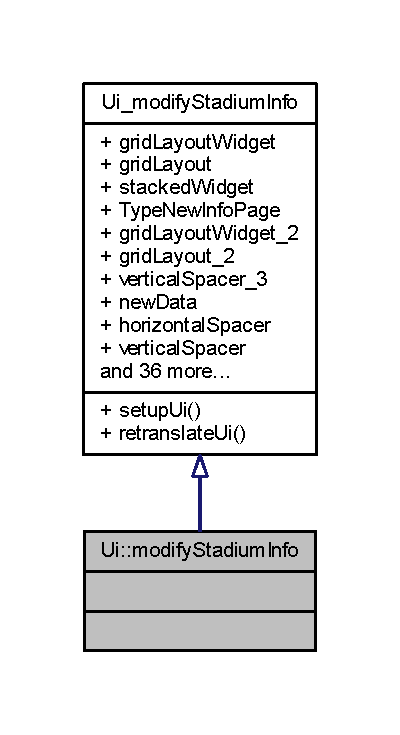
\includegraphics[width=192pt]{class_ui_1_1modify_stadium_info__inherit__graph}
\end{center}
\end{figure}


Collaboration diagram for Ui\+:\+:modify\+Stadium\+Info\+:\nopagebreak
\begin{figure}[H]
\begin{center}
\leavevmode
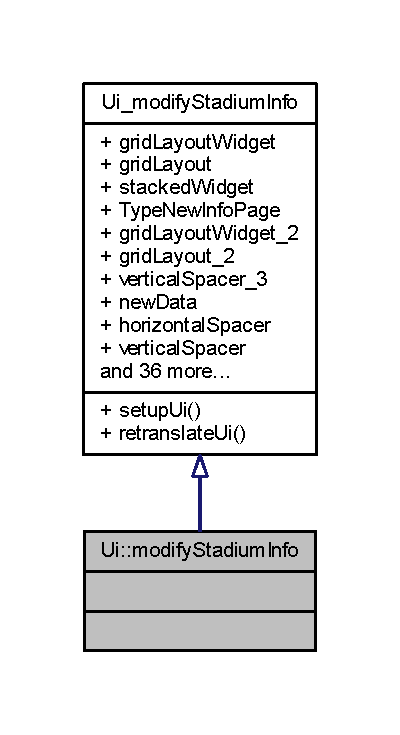
\includegraphics[width=192pt]{class_ui_1_1modify_stadium_info__coll__graph}
\end{center}
\end{figure}
\subsection*{Additional Inherited Members}


The documentation for this class was generated from the following file\+:\begin{DoxyCompactItemize}
\item 
ui\+\_\+modifystadiuminfo.\+h\end{DoxyCompactItemize}

\hypertarget{classmodify_stadium_info}{}\section{modify\+Stadium\+Info Class Reference}
\label{classmodify_stadium_info}\index{modify\+Stadium\+Info@{modify\+Stadium\+Info}}


Inheritance diagram for modify\+Stadium\+Info\+:\nopagebreak
\begin{figure}[H]
\begin{center}
\leavevmode
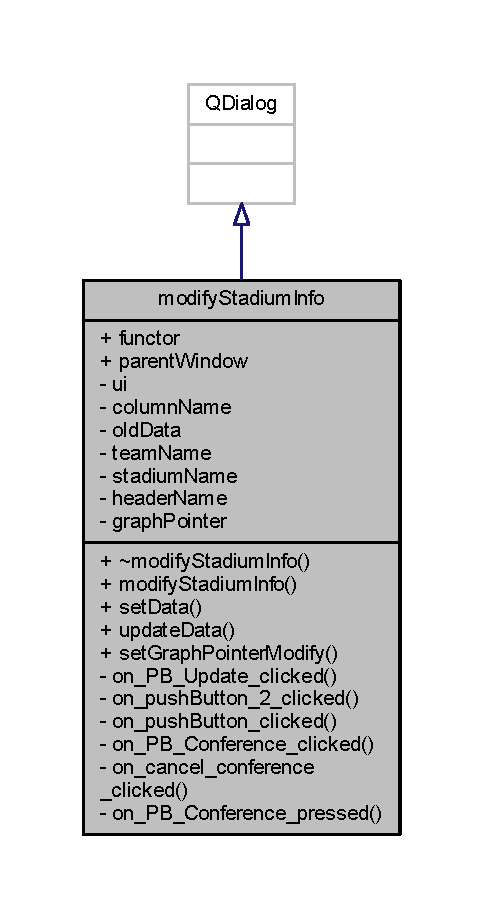
\includegraphics[width=232pt]{classmodify_stadium_info__inherit__graph}
\end{center}
\end{figure}


Collaboration diagram for modify\+Stadium\+Info\+:\nopagebreak
\begin{figure}[H]
\begin{center}
\leavevmode
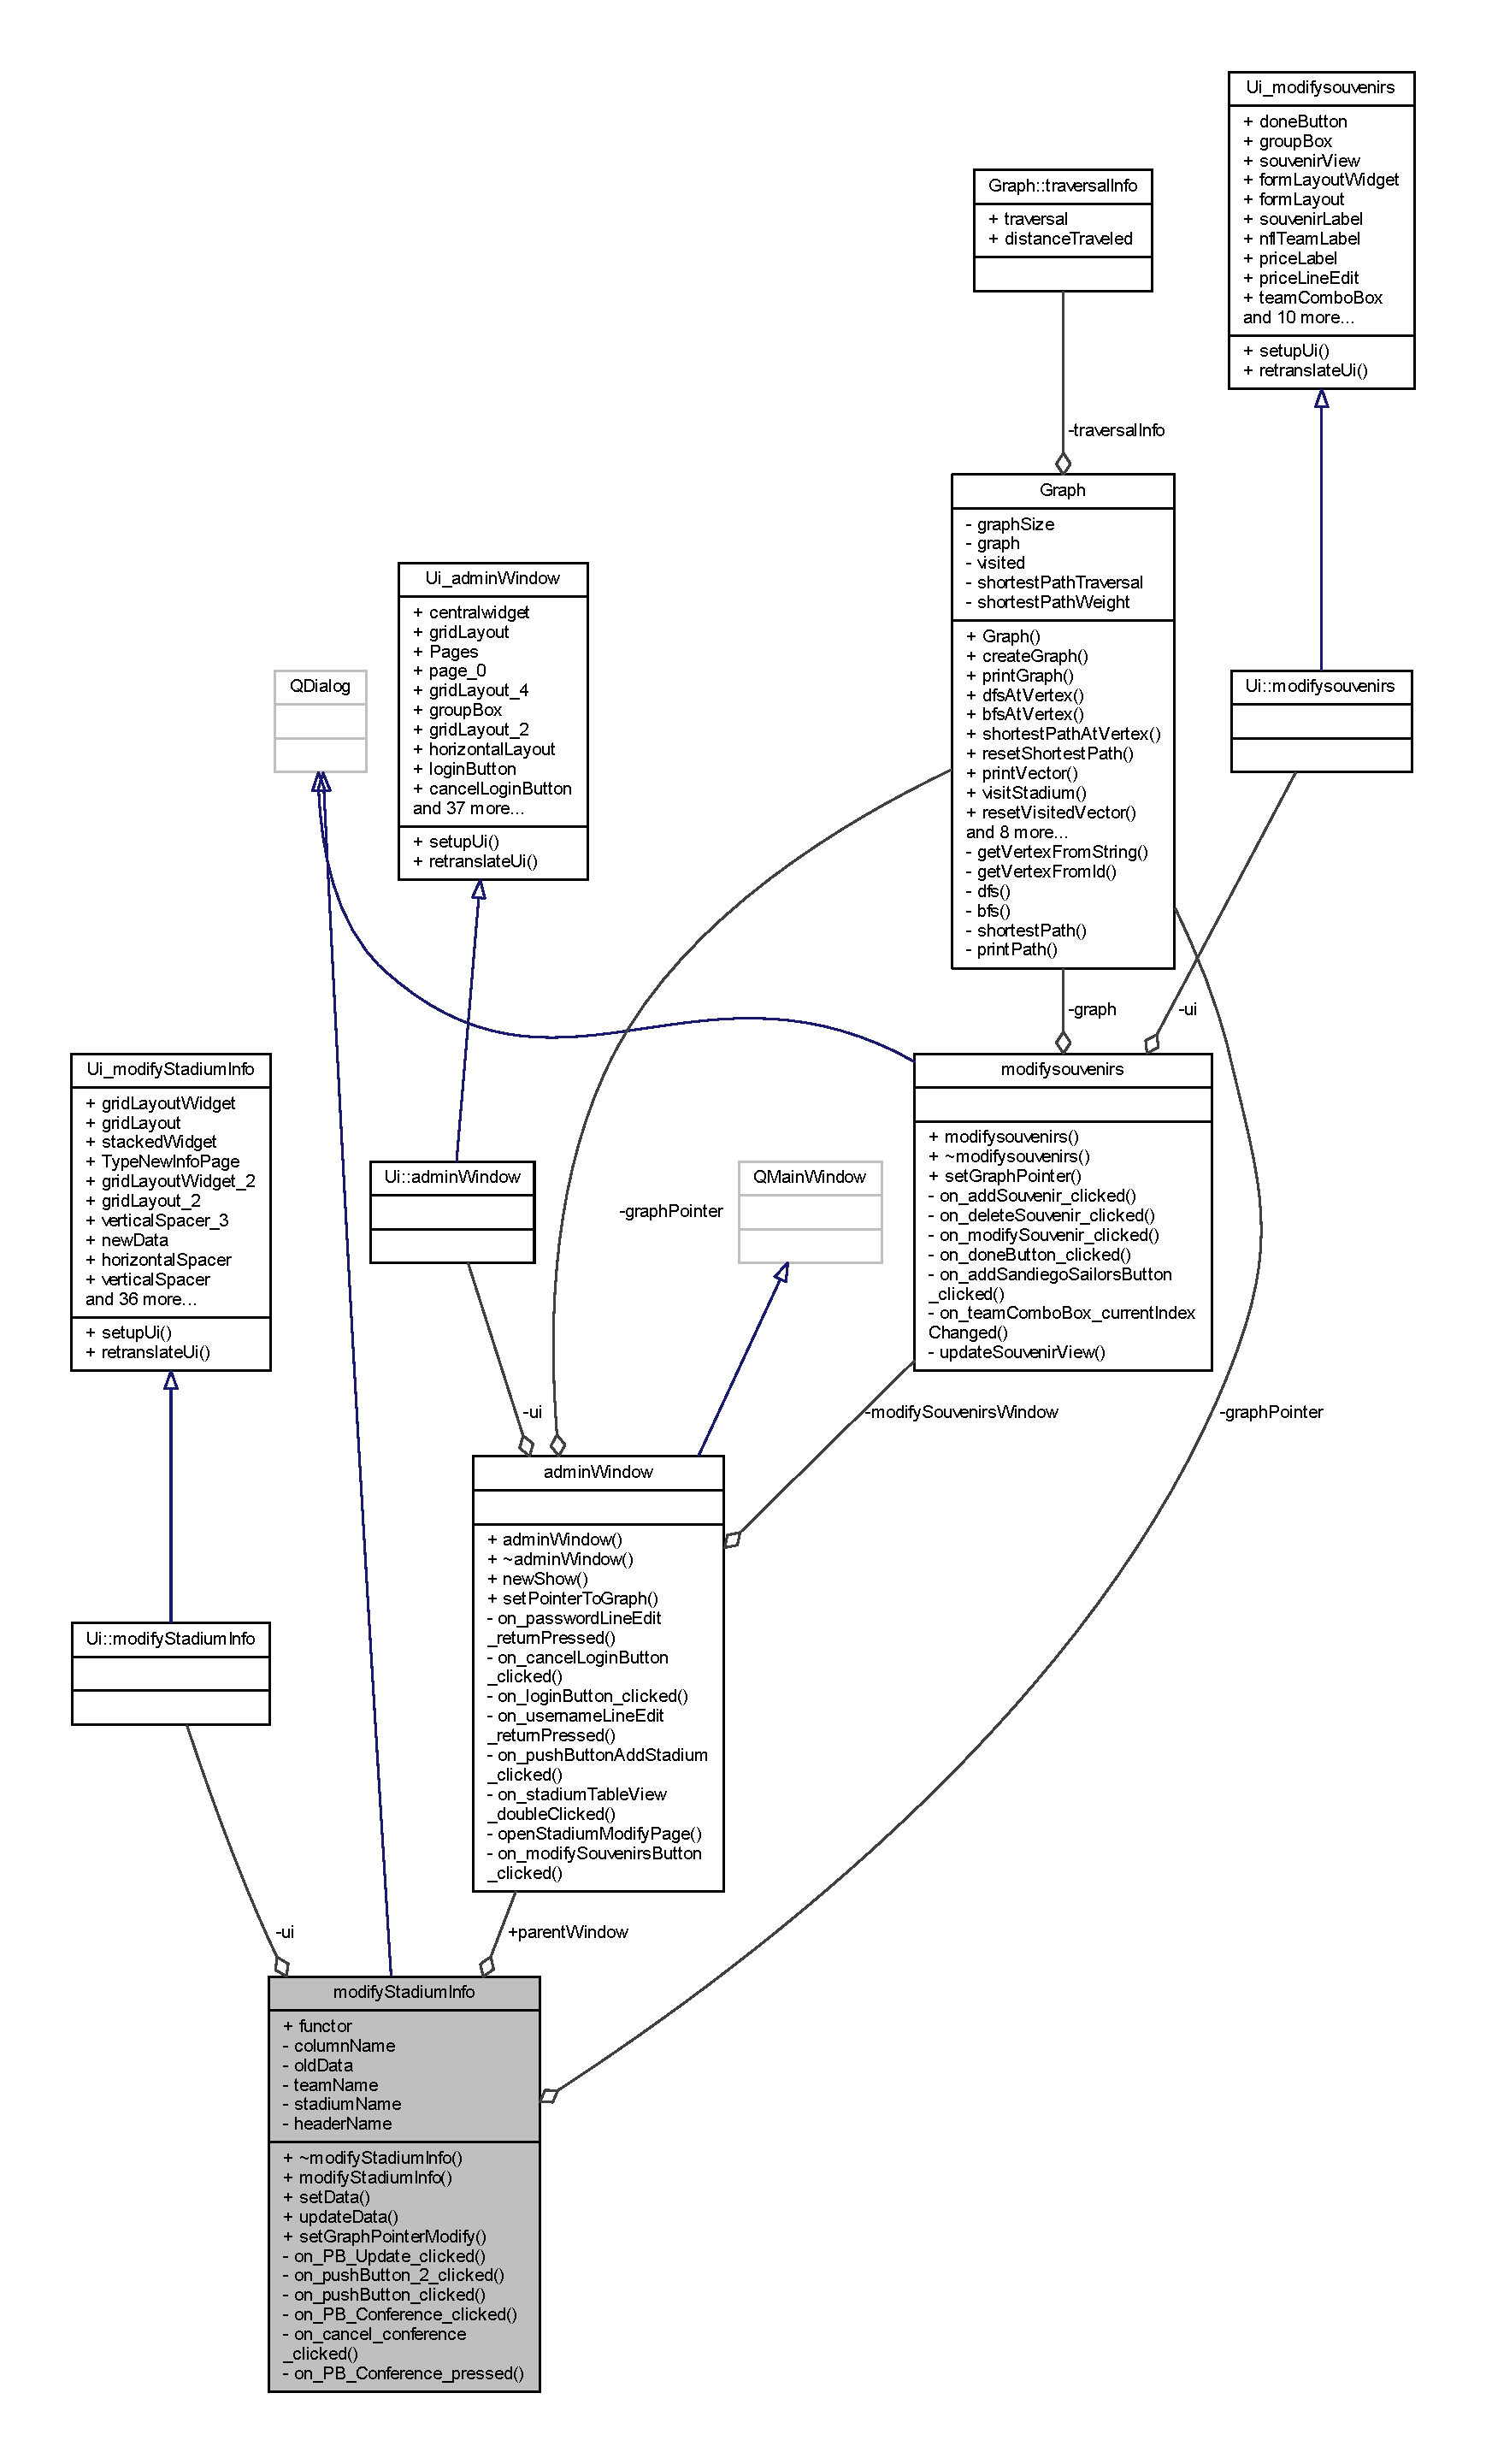
\includegraphics[height=550pt]{classmodify_stadium_info__coll__graph}
\end{center}
\end{figure}
\subsection*{Public Types}
\begin{DoxyCompactItemize}
\item 
\mbox{\Hypertarget{classmodify_stadium_info_aa54c08275884b7295007eff22fa722cc}\label{classmodify_stadium_info_aa54c08275884b7295007eff22fa722cc}} 
typedef void(admin\+Window\+::$\ast$ {\bfseries function\+Name}) ()
\end{DoxyCompactItemize}
\subsection*{Public Member Functions}
\begin{DoxyCompactItemize}
\item 
\mbox{\Hypertarget{classmodify_stadium_info_a28e8ff87dc2589700da092d7d0b5a5e9}\label{classmodify_stadium_info_a28e8ff87dc2589700da092d7d0b5a5e9}} 
{\bfseries modify\+Stadium\+Info} (\hyperlink{classadmin_window}{admin\+Window} \&pw, function\+Name funcF)
\item 
\mbox{\Hypertarget{classmodify_stadium_info_a47d51d5e2efd12621222cba246b54181}\label{classmodify_stadium_info_a47d51d5e2efd12621222cba246b54181}} 
void {\bfseries set\+Data} (Q\+String old\+Data, Q\+String team, Q\+String stadium, Q\+String column, Q\+String header)
\item 
\mbox{\Hypertarget{classmodify_stadium_info_a361c1b7b1b10d30de434c8dd2e2570b5}\label{classmodify_stadium_info_a361c1b7b1b10d30de434c8dd2e2570b5}} 
void {\bfseries update\+Data} (Q\+String)
\item 
\mbox{\Hypertarget{classmodify_stadium_info_a93aecdd05414df698c4998ed6baa16d1}\label{classmodify_stadium_info_a93aecdd05414df698c4998ed6baa16d1}} 
void {\bfseries set\+Graph\+Pointer\+Modify} (\hyperlink{class_graph}{Graph} $\ast$g)
\end{DoxyCompactItemize}
\subsection*{Public Attributes}
\begin{DoxyCompactItemize}
\item 
\mbox{\Hypertarget{classmodify_stadium_info_ab32435bf01e518d616cff085b9de5831}\label{classmodify_stadium_info_ab32435bf01e518d616cff085b9de5831}} 
function\+Name {\bfseries functor}
\item 
\mbox{\Hypertarget{classmodify_stadium_info_a8aeef91cabb8db2b4b3810cd0aaa14a4}\label{classmodify_stadium_info_a8aeef91cabb8db2b4b3810cd0aaa14a4}} 
\hyperlink{classadmin_window}{admin\+Window} \& {\bfseries parent\+Window}
\end{DoxyCompactItemize}
\subsection*{Private Slots}
\begin{DoxyCompactItemize}
\item 
\mbox{\Hypertarget{classmodify_stadium_info_a22af306c4ec113b980764cbc434121d7}\label{classmodify_stadium_info_a22af306c4ec113b980764cbc434121d7}} 
void {\bfseries on\+\_\+\+P\+B\+\_\+\+Update\+\_\+clicked} ()
\item 
\mbox{\Hypertarget{classmodify_stadium_info_ab76af639ca542e2c067674a50da82f69}\label{classmodify_stadium_info_ab76af639ca542e2c067674a50da82f69}} 
void {\bfseries on\+\_\+push\+Button\+\_\+2\+\_\+clicked} ()
\item 
\mbox{\Hypertarget{classmodify_stadium_info_a80877d8967425a8654a5aa62eecf3412}\label{classmodify_stadium_info_a80877d8967425a8654a5aa62eecf3412}} 
void {\bfseries on\+\_\+push\+Button\+\_\+clicked} ()
\item 
\mbox{\Hypertarget{classmodify_stadium_info_aebbbe8574a0c7bca07a8f297412a1cdd}\label{classmodify_stadium_info_aebbbe8574a0c7bca07a8f297412a1cdd}} 
void {\bfseries on\+\_\+\+P\+B\+\_\+\+Conference\+\_\+clicked} ()
\item 
\mbox{\Hypertarget{classmodify_stadium_info_a3342812eadbf4f305cf9e2c500974c23}\label{classmodify_stadium_info_a3342812eadbf4f305cf9e2c500974c23}} 
void {\bfseries on\+\_\+cancel\+\_\+conference\+\_\+clicked} ()
\item 
\mbox{\Hypertarget{classmodify_stadium_info_a30f2b386fd45a884382372c95a80c330}\label{classmodify_stadium_info_a30f2b386fd45a884382372c95a80c330}} 
void {\bfseries on\+\_\+\+P\+B\+\_\+\+Conference\+\_\+pressed} ()
\end{DoxyCompactItemize}
\subsection*{Private Attributes}
\begin{DoxyCompactItemize}
\item 
\mbox{\Hypertarget{classmodify_stadium_info_a10921671cbb93fe25e5db567cf2f8dc7}\label{classmodify_stadium_info_a10921671cbb93fe25e5db567cf2f8dc7}} 
\hyperlink{class_ui_1_1modify_stadium_info}{Ui\+::modify\+Stadium\+Info} $\ast$ {\bfseries ui}
\item 
\mbox{\Hypertarget{classmodify_stadium_info_a68547f655a7f4bc840e578c5de3593a9}\label{classmodify_stadium_info_a68547f655a7f4bc840e578c5de3593a9}} 
Q\+String {\bfseries column\+Name}
\item 
\mbox{\Hypertarget{classmodify_stadium_info_a1d14f67075046a43a14e975ad6c83f42}\label{classmodify_stadium_info_a1d14f67075046a43a14e975ad6c83f42}} 
Q\+String {\bfseries old\+Data}
\item 
\mbox{\Hypertarget{classmodify_stadium_info_a726677f98d05e27240a8cc03abae610d}\label{classmodify_stadium_info_a726677f98d05e27240a8cc03abae610d}} 
Q\+String {\bfseries team\+Name}
\item 
\mbox{\Hypertarget{classmodify_stadium_info_ade8d9485377ee4463c185dec5e3578ba}\label{classmodify_stadium_info_ade8d9485377ee4463c185dec5e3578ba}} 
Q\+String {\bfseries stadium\+Name}
\item 
\mbox{\Hypertarget{classmodify_stadium_info_a1279d3056e97969d6acb39662175449e}\label{classmodify_stadium_info_a1279d3056e97969d6acb39662175449e}} 
Q\+String {\bfseries header\+Name}
\item 
\mbox{\Hypertarget{classmodify_stadium_info_a2c1ff2aca89b2d5bf2e945475ae01ed3}\label{classmodify_stadium_info_a2c1ff2aca89b2d5bf2e945475ae01ed3}} 
\hyperlink{class_graph}{Graph} $\ast$ {\bfseries graph\+Pointer}
\end{DoxyCompactItemize}


The documentation for this class was generated from the following files\+:\begin{DoxyCompactItemize}
\item 
modifystadiuminfo.\+h\item 
modifystadiuminfo.\+cpp\end{DoxyCompactItemize}

\hypertarget{class_purchase}{}\section{Purchase Class Reference}
\label{class_purchase}\index{Purchase@{Purchase}}


Collaboration diagram for Purchase\+:\nopagebreak
\begin{figure}[H]
\begin{center}
\leavevmode
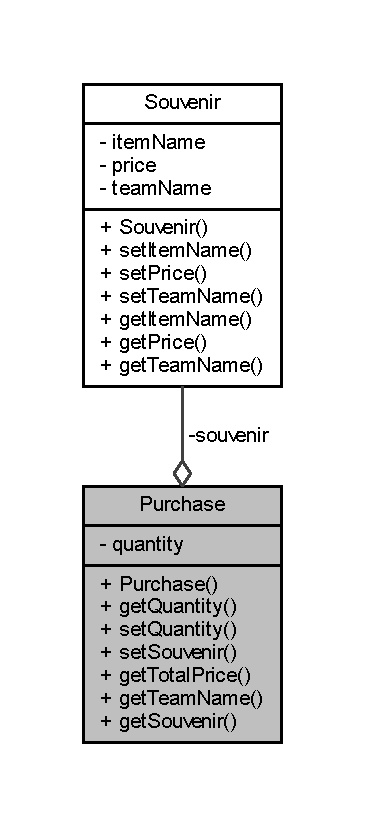
\includegraphics[width=175pt]{class_purchase__coll__graph}
\end{center}
\end{figure}
\subsection*{Public Member Functions}
\begin{DoxyCompactItemize}
\item 
\mbox{\Hypertarget{class_purchase_affdd7456d399278a348ae2e26f8928dd}\label{class_purchase_affdd7456d399278a348ae2e26f8928dd}} 
int {\bfseries get\+Quantity} ()
\item 
\mbox{\Hypertarget{class_purchase_ad5dc255665b0986b11da43ad6ce06b3c}\label{class_purchase_ad5dc255665b0986b11da43ad6ce06b3c}} 
void {\bfseries set\+Quantity} (double)
\item 
\mbox{\Hypertarget{class_purchase_a26156457fb62097acd3341d7f8e2d14d}\label{class_purchase_a26156457fb62097acd3341d7f8e2d14d}} 
void {\bfseries set\+Souvenir} (\hyperlink{class_souvenir}{Souvenir} s)
\item 
\mbox{\Hypertarget{class_purchase_a49adb5a9c4c972faef2bb0dfbfd9327c}\label{class_purchase_a49adb5a9c4c972faef2bb0dfbfd9327c}} 
double {\bfseries get\+Total\+Price} () const
\item 
\mbox{\Hypertarget{class_purchase_aae64c12f19f832c742ae036ab0785d89}\label{class_purchase_aae64c12f19f832c742ae036ab0785d89}} 
Q\+String {\bfseries get\+Team\+Name} () const
\item 
\mbox{\Hypertarget{class_purchase_a49f7cf68192e2bb37faa394cde681ee9}\label{class_purchase_a49f7cf68192e2bb37faa394cde681ee9}} 
Q\+String {\bfseries get\+Souvenir} ()
\end{DoxyCompactItemize}
\subsection*{Private Attributes}
\begin{DoxyCompactItemize}
\item 
\mbox{\Hypertarget{class_purchase_ad5c7f4e47489000e1514211b7d219fe7}\label{class_purchase_ad5c7f4e47489000e1514211b7d219fe7}} 
\hyperlink{class_souvenir}{Souvenir} {\bfseries souvenir}
\item 
\mbox{\Hypertarget{class_purchase_a2ba21ff1de4cec6e51acad3d6a92d73a}\label{class_purchase_a2ba21ff1de4cec6e51acad3d6a92d73a}} 
int {\bfseries quantity}
\end{DoxyCompactItemize}


The documentation for this class was generated from the following files\+:\begin{DoxyCompactItemize}
\item 
purchase.\+h\item 
purchase.\+cpp\end{DoxyCompactItemize}

\hypertarget{class_souvenir}{}\section{Souvenir Class Reference}
\label{class_souvenir}\index{Souvenir@{Souvenir}}


Collaboration diagram for Souvenir\+:
\nopagebreak
\begin{figure}[H]
\begin{center}
\leavevmode
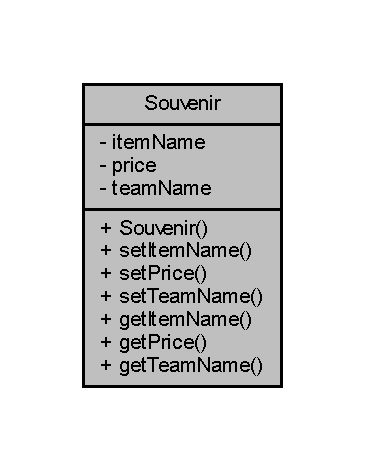
\includegraphics[width=175pt]{class_souvenir__coll__graph}
\end{center}
\end{figure}
\subsection*{Public Member Functions}
\begin{DoxyCompactItemize}
\item 
\mbox{\Hypertarget{class_souvenir_a968ad05d980d8284b891d760b4338553}\label{class_souvenir_a968ad05d980d8284b891d760b4338553}} 
void {\bfseries set\+Item\+Name} (Q\+String)
\item 
\mbox{\Hypertarget{class_souvenir_a3664ce2aa3d258e6bf21e2f0f3741efe}\label{class_souvenir_a3664ce2aa3d258e6bf21e2f0f3741efe}} 
void {\bfseries set\+Price} (double price)
\item 
\mbox{\Hypertarget{class_souvenir_aadd5431a88f683445ce407cbfd4b0390}\label{class_souvenir_aadd5431a88f683445ce407cbfd4b0390}} 
void {\bfseries set\+Team\+Name} (Q\+String name)
\item 
\mbox{\Hypertarget{class_souvenir_a0b74aa98dac5f6d6b2541752ec431a82}\label{class_souvenir_a0b74aa98dac5f6d6b2541752ec431a82}} 
Q\+String {\bfseries get\+Item\+Name} () const
\item 
\mbox{\Hypertarget{class_souvenir_aa3dfe5b64bfc5e3785cefd90759e281f}\label{class_souvenir_aa3dfe5b64bfc5e3785cefd90759e281f}} 
double {\bfseries get\+Price} () const
\item 
\mbox{\Hypertarget{class_souvenir_ab52b658cab6e30ca568a70df08797d8c}\label{class_souvenir_ab52b658cab6e30ca568a70df08797d8c}} 
Q\+String {\bfseries get\+Team\+Name} () const
\end{DoxyCompactItemize}
\subsection*{Private Attributes}
\begin{DoxyCompactItemize}
\item 
\mbox{\Hypertarget{class_souvenir_adbd556e3c1c0404bf71ea1d87100c091}\label{class_souvenir_adbd556e3c1c0404bf71ea1d87100c091}} 
Q\+String {\bfseries item\+Name}
\item 
\mbox{\Hypertarget{class_souvenir_a2991e814ee69fba3a86d90b7ea48cb2b}\label{class_souvenir_a2991e814ee69fba3a86d90b7ea48cb2b}} 
double {\bfseries price}
\item 
\mbox{\Hypertarget{class_souvenir_a134e714c71e99d082304e0e332d5ce0d}\label{class_souvenir_a134e714c71e99d082304e0e332d5ce0d}} 
Q\+String {\bfseries team\+Name}
\end{DoxyCompactItemize}


The documentation for this class was generated from the following files\+:\begin{DoxyCompactItemize}
\item 
souvenir.\+h\item 
souvenir.\+cpp\end{DoxyCompactItemize}

\hypertarget{struct_graph_1_1traversal_info}{}\section{Graph\+:\+:traversal\+Info Struct Reference}
\label{struct_graph_1_1traversal_info}\index{Graph\+::traversal\+Info@{Graph\+::traversal\+Info}}


Collaboration diagram for Graph\+:\+:traversal\+Info\+:\nopagebreak
\begin{figure}[H]
\begin{center}
\leavevmode
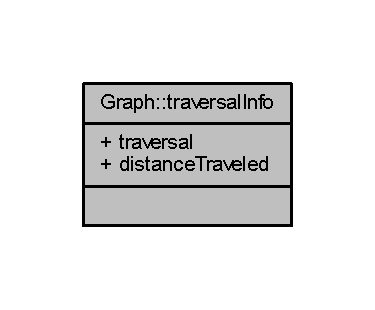
\includegraphics[width=180pt]{struct_graph_1_1traversal_info__coll__graph}
\end{center}
\end{figure}
\subsection*{Public Attributes}
\begin{DoxyCompactItemize}
\item 
\mbox{\Hypertarget{struct_graph_1_1traversal_info_a6cc0cefaf64ee80392f52df1e3b98718}\label{struct_graph_1_1traversal_info_a6cc0cefaf64ee80392f52df1e3b98718}} 
Q\+String\+List {\bfseries traversal}
\item 
\mbox{\Hypertarget{struct_graph_1_1traversal_info_aad37277396b6c83b5e1ea23d5052e098}\label{struct_graph_1_1traversal_info_aad37277396b6c83b5e1ea23d5052e098}} 
int {\bfseries distance\+Traveled}
\end{DoxyCompactItemize}


The documentation for this struct was generated from the following file\+:\begin{DoxyCompactItemize}
\item 
graph.\+h\end{DoxyCompactItemize}

\hypertarget{class_ui__admin_window}{}\section{Ui\+\_\+admin\+Window Class Reference}
\label{class_ui__admin_window}\index{Ui\+\_\+admin\+Window@{Ui\+\_\+admin\+Window}}


Inheritance diagram for Ui\+\_\+admin\+Window\+:\nopagebreak
\begin{figure}[H]
\begin{center}
\leavevmode
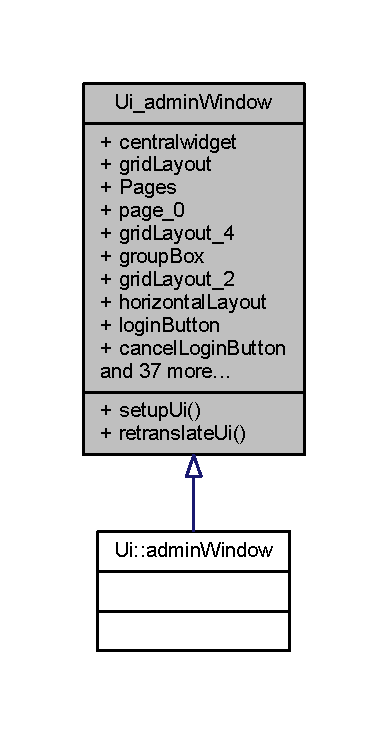
\includegraphics[width=186pt]{class_ui__admin_window__inherit__graph}
\end{center}
\end{figure}


Collaboration diagram for Ui\+\_\+admin\+Window\+:\nopagebreak
\begin{figure}[H]
\begin{center}
\leavevmode
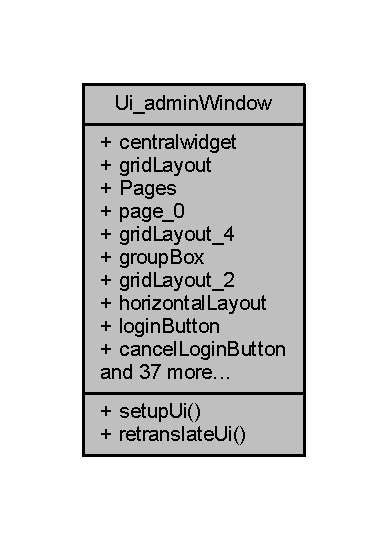
\includegraphics[width=186pt]{class_ui__admin_window__coll__graph}
\end{center}
\end{figure}
\subsection*{Public Member Functions}
\begin{DoxyCompactItemize}
\item 
\mbox{\Hypertarget{class_ui__admin_window_a7057c6fc6718b89da0d1ef1e8feb5e62}\label{class_ui__admin_window_a7057c6fc6718b89da0d1ef1e8feb5e62}} 
void {\bfseries setup\+Ui} (Q\+Main\+Window $\ast$\hyperlink{classadmin_window}{admin\+Window})
\item 
\mbox{\Hypertarget{class_ui__admin_window_ac7535c816a61f0c9b55d8d8fbe774130}\label{class_ui__admin_window_ac7535c816a61f0c9b55d8d8fbe774130}} 
void {\bfseries retranslate\+Ui} (Q\+Main\+Window $\ast$\hyperlink{classadmin_window}{admin\+Window})
\end{DoxyCompactItemize}
\subsection*{Public Attributes}
\begin{DoxyCompactItemize}
\item 
\mbox{\Hypertarget{class_ui__admin_window_ad17f51669733a04a3298e884a350194b}\label{class_ui__admin_window_ad17f51669733a04a3298e884a350194b}} 
Q\+Widget $\ast$ {\bfseries centralwidget}
\item 
\mbox{\Hypertarget{class_ui__admin_window_aa3a79e2d7edd5d88b73ccbbba6e0c92d}\label{class_ui__admin_window_aa3a79e2d7edd5d88b73ccbbba6e0c92d}} 
Q\+Grid\+Layout $\ast$ {\bfseries grid\+Layout}
\item 
\mbox{\Hypertarget{class_ui__admin_window_a13ee2305bf4bdd76d36e4cf0222c5069}\label{class_ui__admin_window_a13ee2305bf4bdd76d36e4cf0222c5069}} 
Q\+Stacked\+Widget $\ast$ {\bfseries Pages}
\item 
\mbox{\Hypertarget{class_ui__admin_window_a43315add4afee6168fa9ada5e3ef1dbe}\label{class_ui__admin_window_a43315add4afee6168fa9ada5e3ef1dbe}} 
Q\+Widget $\ast$ {\bfseries page\+\_\+0}
\item 
\mbox{\Hypertarget{class_ui__admin_window_a2e6136e8cebb19db3f32870556391d04}\label{class_ui__admin_window_a2e6136e8cebb19db3f32870556391d04}} 
Q\+Grid\+Layout $\ast$ {\bfseries grid\+Layout\+\_\+4}
\item 
\mbox{\Hypertarget{class_ui__admin_window_a160899f1a14d8bf803aca76f9fd28bfd}\label{class_ui__admin_window_a160899f1a14d8bf803aca76f9fd28bfd}} 
Q\+Group\+Box $\ast$ {\bfseries group\+Box}
\item 
\mbox{\Hypertarget{class_ui__admin_window_a4177cf23c76973765b5de9df513f98c0}\label{class_ui__admin_window_a4177cf23c76973765b5de9df513f98c0}} 
Q\+Grid\+Layout $\ast$ {\bfseries grid\+Layout\+\_\+2}
\item 
\mbox{\Hypertarget{class_ui__admin_window_ab0dedb04b39cd934a969d61be8333e69}\label{class_ui__admin_window_ab0dedb04b39cd934a969d61be8333e69}} 
Q\+H\+Box\+Layout $\ast$ {\bfseries horizontal\+Layout}
\item 
\mbox{\Hypertarget{class_ui__admin_window_a2ca0970e8d04aa05e5111e8ab01d6756}\label{class_ui__admin_window_a2ca0970e8d04aa05e5111e8ab01d6756}} 
Q\+Push\+Button $\ast$ {\bfseries login\+Button}
\item 
\mbox{\Hypertarget{class_ui__admin_window_a4d344ddf2dcc0bd7d9a08f24907c4863}\label{class_ui__admin_window_a4d344ddf2dcc0bd7d9a08f24907c4863}} 
Q\+Push\+Button $\ast$ {\bfseries cancel\+Login\+Button}
\item 
\mbox{\Hypertarget{class_ui__admin_window_aa564254c32ae506e322cee50b4409d95}\label{class_ui__admin_window_aa564254c32ae506e322cee50b4409d95}} 
Q\+Label $\ast$ {\bfseries username\+Label}
\item 
\mbox{\Hypertarget{class_ui__admin_window_a1d36ae0310eafdc93055db14335ed163}\label{class_ui__admin_window_a1d36ae0310eafdc93055db14335ed163}} 
Q\+Line\+Edit $\ast$ {\bfseries username\+Line\+Edit}
\item 
\mbox{\Hypertarget{class_ui__admin_window_a9dec41198fbd9b40fc61ca88ec6ee061}\label{class_ui__admin_window_a9dec41198fbd9b40fc61ca88ec6ee061}} 
Q\+Label $\ast$ {\bfseries password\+Label}
\item 
\mbox{\Hypertarget{class_ui__admin_window_a919d6f5c3587625cbfc8db868f0dd812}\label{class_ui__admin_window_a919d6f5c3587625cbfc8db868f0dd812}} 
Q\+Label $\ast$ {\bfseries label}
\item 
\mbox{\Hypertarget{class_ui__admin_window_a57114baa83c61780018d751e07062a97}\label{class_ui__admin_window_a57114baa83c61780018d751e07062a97}} 
Q\+Line\+Edit $\ast$ {\bfseries password\+Line\+Edit}
\item 
\mbox{\Hypertarget{class_ui__admin_window_a72160c7881ba470d56f22daee59bd7fe}\label{class_ui__admin_window_a72160c7881ba470d56f22daee59bd7fe}} 
Q\+Spacer\+Item $\ast$ {\bfseries vertical\+Spacer}
\item 
\mbox{\Hypertarget{class_ui__admin_window_a493a4cd123a27314aa560943b2b82e8a}\label{class_ui__admin_window_a493a4cd123a27314aa560943b2b82e8a}} 
Q\+Spacer\+Item $\ast$ {\bfseries horizontal\+Spacer}
\item 
\mbox{\Hypertarget{class_ui__admin_window_a85db55755f6b56a83fe29a70cac8d840}\label{class_ui__admin_window_a85db55755f6b56a83fe29a70cac8d840}} 
Q\+Spacer\+Item $\ast$ {\bfseries horizontal\+Spacer\+\_\+2}
\item 
\mbox{\Hypertarget{class_ui__admin_window_a685db74b3f59229f940f1c3c23b2c936}\label{class_ui__admin_window_a685db74b3f59229f940f1c3c23b2c936}} 
Q\+Spacer\+Item $\ast$ {\bfseries vertical\+Spacer\+\_\+2}
\item 
\mbox{\Hypertarget{class_ui__admin_window_a5f660fd795ea4bd14f8dbe216ba52f9f}\label{class_ui__admin_window_a5f660fd795ea4bd14f8dbe216ba52f9f}} 
Q\+Widget $\ast$ {\bfseries page\+\_\+1}
\item 
\mbox{\Hypertarget{class_ui__admin_window_ab0b3e24daf07c88592633608565f531d}\label{class_ui__admin_window_ab0b3e24daf07c88592633608565f531d}} 
Q\+Grid\+Layout $\ast$ {\bfseries grid\+Layout\+\_\+3}
\item 
\mbox{\Hypertarget{class_ui__admin_window_ae5d18ecbdfb7500e8c6d7c6b4a70c9f8}\label{class_ui__admin_window_ae5d18ecbdfb7500e8c6d7c6b4a70c9f8}} 
Q\+V\+Box\+Layout $\ast$ {\bfseries vertical\+Layout\+\_\+5}
\item 
\mbox{\Hypertarget{class_ui__admin_window_a1930c7f889bb35385685ca06e7e75c1b}\label{class_ui__admin_window_a1930c7f889bb35385685ca06e7e75c1b}} 
Q\+Label $\ast$ {\bfseries label\+\_\+23}
\item 
\mbox{\Hypertarget{class_ui__admin_window_a395db14e2469224c2660371b42cf5bac}\label{class_ui__admin_window_a395db14e2469224c2660371b42cf5bac}} 
Q\+Label $\ast$ {\bfseries label\+\_\+24}
\item 
\mbox{\Hypertarget{class_ui__admin_window_a5c93179d396766560428fa3f792d9c9d}\label{class_ui__admin_window_a5c93179d396766560428fa3f792d9c9d}} 
Q\+Line\+Edit $\ast$ {\bfseries line\+Edit\+Team\+Name}
\item 
\mbox{\Hypertarget{class_ui__admin_window_a3c781499e8fd8108412ac0da86ea786e}\label{class_ui__admin_window_a3c781499e8fd8108412ac0da86ea786e}} 
Q\+Label $\ast$ {\bfseries label\+\_\+25}
\item 
\mbox{\Hypertarget{class_ui__admin_window_ab9140c919d2ab355f158447615fd0879}\label{class_ui__admin_window_ab9140c919d2ab355f158447615fd0879}} 
Q\+Line\+Edit $\ast$ {\bfseries line\+Edit\+Stadium\+Name}
\item 
\mbox{\Hypertarget{class_ui__admin_window_a401b7b33afb09c40ba6ad51f9e04e3c5}\label{class_ui__admin_window_a401b7b33afb09c40ba6ad51f9e04e3c5}} 
Q\+Label $\ast$ {\bfseries label\+\_\+26}
\item 
\mbox{\Hypertarget{class_ui__admin_window_ad62c58f1068b9e36e7e7ceccf628e5b6}\label{class_ui__admin_window_ad62c58f1068b9e36e7e7ceccf628e5b6}} 
Q\+Line\+Edit $\ast$ {\bfseries line\+Edit\+Seating\+Cap}
\item 
\mbox{\Hypertarget{class_ui__admin_window_aa3a13ca78b8adc97ae4ead8b7d492fdf}\label{class_ui__admin_window_aa3a13ca78b8adc97ae4ead8b7d492fdf}} 
Q\+Label $\ast$ {\bfseries label\+\_\+27}
\item 
\mbox{\Hypertarget{class_ui__admin_window_a119c844eeadafd1ea61882b93cfd4368}\label{class_ui__admin_window_a119c844eeadafd1ea61882b93cfd4368}} 
Q\+Line\+Edit $\ast$ {\bfseries line\+Edit\+Location}
\item 
\mbox{\Hypertarget{class_ui__admin_window_a305f3685f7b0c18c25da1d9bf2fc9f0b}\label{class_ui__admin_window_a305f3685f7b0c18c25da1d9bf2fc9f0b}} 
Q\+Label $\ast$ {\bfseries label\+\_\+31}
\item 
\mbox{\Hypertarget{class_ui__admin_window_a23d9625e7f2062fbe3565c97cf9ce13b}\label{class_ui__admin_window_a23d9625e7f2062fbe3565c97cf9ce13b}} 
Q\+Combo\+Box $\ast$ {\bfseries combo\+Box\+Conference}
\item 
\mbox{\Hypertarget{class_ui__admin_window_afa345e3e10efcf1f4fb490e2548978ab}\label{class_ui__admin_window_afa345e3e10efcf1f4fb490e2548978ab}} 
Q\+Label $\ast$ {\bfseries label\+\_\+29}
\item 
\mbox{\Hypertarget{class_ui__admin_window_a23d784ce5e0c7a0713a690aadef0d20c}\label{class_ui__admin_window_a23d784ce5e0c7a0713a690aadef0d20c}} 
Q\+Line\+Edit $\ast$ {\bfseries line\+Edit\+Surface\+Type}
\item 
\mbox{\Hypertarget{class_ui__admin_window_a10add1b74b41da50a7f67c844bac7e0d}\label{class_ui__admin_window_a10add1b74b41da50a7f67c844bac7e0d}} 
Q\+Label $\ast$ {\bfseries label\+\_\+28}
\item 
\mbox{\Hypertarget{class_ui__admin_window_a75eebcfed5f191ee738faff0d5472098}\label{class_ui__admin_window_a75eebcfed5f191ee738faff0d5472098}} 
Q\+Combo\+Box $\ast$ {\bfseries combo\+Box\+Roof\+Type}
\item 
\mbox{\Hypertarget{class_ui__admin_window_aa4342940f3c54c82c1ccdbc02740b8fd}\label{class_ui__admin_window_aa4342940f3c54c82c1ccdbc02740b8fd}} 
Q\+Label $\ast$ {\bfseries label\+\_\+30}
\item 
\mbox{\Hypertarget{class_ui__admin_window_a86ae0311217da011dabb34aa29f8378f}\label{class_ui__admin_window_a86ae0311217da011dabb34aa29f8378f}} 
Q\+Line\+Edit $\ast$ {\bfseries line\+Edit\+Star\+Pleyer}
\item 
\mbox{\Hypertarget{class_ui__admin_window_ab209c2b00ff53cd2cf0125f41d4337a9}\label{class_ui__admin_window_ab209c2b00ff53cd2cf0125f41d4337a9}} 
Q\+Push\+Button $\ast$ {\bfseries push\+Button\+Add\+Stadium}
\item 
\mbox{\Hypertarget{class_ui__admin_window_a5d94627e7f07f98ab7eb59b540e5ee5b}\label{class_ui__admin_window_a5d94627e7f07f98ab7eb59b540e5ee5b}} 
Q\+Spacer\+Item $\ast$ {\bfseries vertical\+Spacer\+\_\+3}
\item 
\mbox{\Hypertarget{class_ui__admin_window_abd6512573cb48d6c6979f9f37be5ac4d}\label{class_ui__admin_window_abd6512573cb48d6c6979f9f37be5ac4d}} 
Q\+Push\+Button $\ast$ {\bfseries modify\+Souvenirs\+Button}
\item 
\mbox{\Hypertarget{class_ui__admin_window_a20adfd8c9b6a39d9545dfed577bf25e7}\label{class_ui__admin_window_a20adfd8c9b6a39d9545dfed577bf25e7}} 
Q\+V\+Box\+Layout $\ast$ {\bfseries vertical\+Layout\+\_\+6}
\item 
\mbox{\Hypertarget{class_ui__admin_window_abdcf692aef6f34db8f184c07807ddcd0}\label{class_ui__admin_window_abdcf692aef6f34db8f184c07807ddcd0}} 
Q\+Label $\ast$ {\bfseries label\+\_\+32}
\item 
\mbox{\Hypertarget{class_ui__admin_window_a926806214476710cc711e82986b9ae0f}\label{class_ui__admin_window_a926806214476710cc711e82986b9ae0f}} 
Q\+Table\+View $\ast$ {\bfseries stadium\+Table\+View}
\item 
\mbox{\Hypertarget{class_ui__admin_window_a98cd502dd8efcf672c2faea2783f3ec4}\label{class_ui__admin_window_a98cd502dd8efcf672c2faea2783f3ec4}} 
Q\+Menu\+Bar $\ast$ {\bfseries menubar}
\item 
\mbox{\Hypertarget{class_ui__admin_window_accb31cc05b2f6f5f6ce1bf13a5a3d210}\label{class_ui__admin_window_accb31cc05b2f6f5f6ce1bf13a5a3d210}} 
Q\+Status\+Bar $\ast$ {\bfseries statusbar}
\end{DoxyCompactItemize}


The documentation for this class was generated from the following file\+:\begin{DoxyCompactItemize}
\item 
ui\+\_\+adminwindow.\+h\end{DoxyCompactItemize}

\hypertarget{class_ui___main_window}{}\section{Ui\+\_\+\+Main\+Window Class Reference}
\label{class_ui___main_window}\index{Ui\+\_\+\+Main\+Window@{Ui\+\_\+\+Main\+Window}}


Inheritance diagram for Ui\+\_\+\+Main\+Window\+:
\nopagebreak
\begin{figure}[H]
\begin{center}
\leavevmode
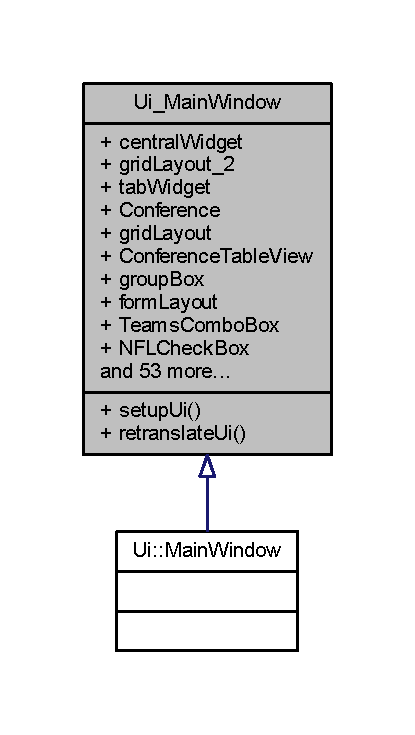
\includegraphics[width=199pt]{class_ui___main_window__inherit__graph}
\end{center}
\end{figure}


Collaboration diagram for Ui\+\_\+\+Main\+Window\+:
\nopagebreak
\begin{figure}[H]
\begin{center}
\leavevmode
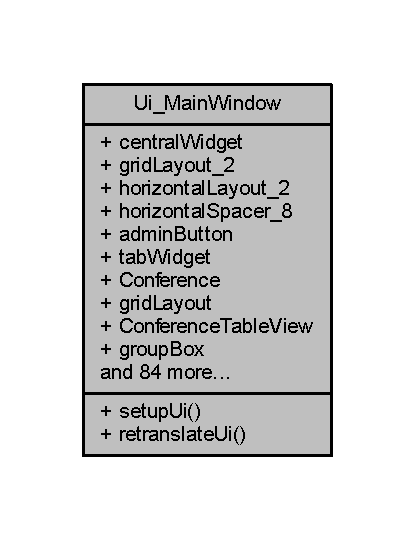
\includegraphics[width=199pt]{class_ui___main_window__coll__graph}
\end{center}
\end{figure}
\subsection*{Public Member Functions}
\begin{DoxyCompactItemize}
\item 
\mbox{\Hypertarget{class_ui___main_window_acf4a0872c4c77d8f43a2ec66ed849b58}\label{class_ui___main_window_acf4a0872c4c77d8f43a2ec66ed849b58}} 
void {\bfseries setup\+Ui} (Q\+Main\+Window $\ast$\hyperlink{class_main_window}{Main\+Window})
\item 
\mbox{\Hypertarget{class_ui___main_window_a097dd160c3534a204904cb374412c618}\label{class_ui___main_window_a097dd160c3534a204904cb374412c618}} 
void {\bfseries retranslate\+Ui} (Q\+Main\+Window $\ast$\hyperlink{class_main_window}{Main\+Window})
\end{DoxyCompactItemize}
\subsection*{Public Attributes}
\begin{DoxyCompactItemize}
\item 
\mbox{\Hypertarget{class_ui___main_window_a30075506c2116c3ed4ff25e07ae75f81}\label{class_ui___main_window_a30075506c2116c3ed4ff25e07ae75f81}} 
Q\+Widget $\ast$ {\bfseries central\+Widget}
\item 
\mbox{\Hypertarget{class_ui___main_window_a6b2a0c5f7e8ff2a87134908dd770d2d2}\label{class_ui___main_window_a6b2a0c5f7e8ff2a87134908dd770d2d2}} 
Q\+Grid\+Layout $\ast$ {\bfseries grid\+Layout\+\_\+2}
\item 
\mbox{\Hypertarget{class_ui___main_window_a3260b943854b841c986f47c4726ee7f9}\label{class_ui___main_window_a3260b943854b841c986f47c4726ee7f9}} 
Q\+Tab\+Widget $\ast$ {\bfseries tab\+Widget}
\item 
\mbox{\Hypertarget{class_ui___main_window_a44599cdae18cc6d9a8ccdb3c4391c8d5}\label{class_ui___main_window_a44599cdae18cc6d9a8ccdb3c4391c8d5}} 
Q\+Widget $\ast$ {\bfseries Conference}
\item 
\mbox{\Hypertarget{class_ui___main_window_a525ed3c5fe0784ac502ee222fba4e205}\label{class_ui___main_window_a525ed3c5fe0784ac502ee222fba4e205}} 
Q\+Grid\+Layout $\ast$ {\bfseries grid\+Layout}
\item 
\mbox{\Hypertarget{class_ui___main_window_ac7686ce338a15a95c55a81860afaa5e1}\label{class_ui___main_window_ac7686ce338a15a95c55a81860afaa5e1}} 
Q\+Table\+View $\ast$ {\bfseries Conference\+Table\+View}
\item 
\mbox{\Hypertarget{class_ui___main_window_aef7cb3be8cecfc9aaf98f036a98781ce}\label{class_ui___main_window_aef7cb3be8cecfc9aaf98f036a98781ce}} 
Q\+Group\+Box $\ast$ {\bfseries group\+Box}
\item 
\mbox{\Hypertarget{class_ui___main_window_afedcce3d8f3dddf4c1fd5b768660b8ee}\label{class_ui___main_window_afedcce3d8f3dddf4c1fd5b768660b8ee}} 
Q\+Form\+Layout $\ast$ {\bfseries form\+Layout}
\item 
\mbox{\Hypertarget{class_ui___main_window_a9616d0f3fbadb2b92314f6d033fff578}\label{class_ui___main_window_a9616d0f3fbadb2b92314f6d033fff578}} 
Q\+Combo\+Box $\ast$ {\bfseries Teams\+Combo\+Box}
\item 
\mbox{\Hypertarget{class_ui___main_window_aebb039e3f09a651f0037929e8acf340e}\label{class_ui___main_window_aebb039e3f09a651f0037929e8acf340e}} 
Q\+Check\+Box $\ast$ {\bfseries N\+F\+L\+Check\+Box}
\item 
\mbox{\Hypertarget{class_ui___main_window_a8a71bb9cb909761b6a601366d5375f38}\label{class_ui___main_window_a8a71bb9cb909761b6a601366d5375f38}} 
Q\+Check\+Box $\ast$ {\bfseries A\+F\+L\+Check\+Box}
\item 
\mbox{\Hypertarget{class_ui___main_window_afc9b813ccebcee47b71c71bb59b165f6}\label{class_ui___main_window_afc9b813ccebcee47b71c71bb59b165f6}} 
Q\+Check\+Box $\ast$ {\bfseries Both\+Check\+Box}
\item 
\mbox{\Hypertarget{class_ui___main_window_ac3a643e401a0dcf0f9bbc8c19f6e01e6}\label{class_ui___main_window_ac3a643e401a0dcf0f9bbc8c19f6e01e6}} 
Q\+Label $\ast$ {\bfseries roof\+Label}
\item 
\mbox{\Hypertarget{class_ui___main_window_a68b8d9f3b085e78f463b84b4a712382b}\label{class_ui___main_window_a68b8d9f3b085e78f463b84b4a712382b}} 
Q\+Combo\+Box $\ast$ {\bfseries roof\+Combo\+Box}
\item 
\mbox{\Hypertarget{class_ui___main_window_a2e2516d755e4dd53fc905dabddf2738a}\label{class_ui___main_window_a2e2516d755e4dd53fc905dabddf2738a}} 
Q\+Label $\ast$ {\bfseries label\+\_\+2}
\item 
\mbox{\Hypertarget{class_ui___main_window_afc5320fcbc22959b1298da9f2cb4559b}\label{class_ui___main_window_afc5320fcbc22959b1298da9f2cb4559b}} 
Q\+Label $\ast$ {\bfseries roof\+Number\+Label}
\item 
\mbox{\Hypertarget{class_ui___main_window_acd6fdc9ebacc4b25b834162380d75ce8}\label{class_ui___main_window_acd6fdc9ebacc4b25b834162380d75ce8}} 
Q\+H\+Box\+Layout $\ast$ {\bfseries horizontal\+Layout}
\item 
\mbox{\Hypertarget{class_ui___main_window_ae2007c6e48638f819d3ac57be8daa4ca}\label{class_ui___main_window_ae2007c6e48638f819d3ac57be8daa4ca}} 
Q\+Spacer\+Item $\ast$ {\bfseries horizontal\+Spacer\+\_\+3}
\item 
\mbox{\Hypertarget{class_ui___main_window_a7871ea8c4b6c595d7ccd53960b344719}\label{class_ui___main_window_a7871ea8c4b6c595d7ccd53960b344719}} 
Q\+Spacer\+Item $\ast$ {\bfseries horizontal\+Spacer}
\item 
\mbox{\Hypertarget{class_ui___main_window_ad9c89133780f28e6efa2ec17ceb9cff5}\label{class_ui___main_window_ad9c89133780f28e6efa2ec17ceb9cff5}} 
Q\+Label $\ast$ {\bfseries label}
\item 
\mbox{\Hypertarget{class_ui___main_window_aeaa664b636e02543a3047acb6d8918c5}\label{class_ui___main_window_aeaa664b636e02543a3047acb6d8918c5}} 
Q\+L\+C\+D\+Number $\ast$ {\bfseries lcd\+Number}
\item 
\mbox{\Hypertarget{class_ui___main_window_a71605bcf74c938f64207451850fc69b1}\label{class_ui___main_window_a71605bcf74c938f64207451850fc69b1}} 
Q\+Spacer\+Item $\ast$ {\bfseries horizontal\+Spacer\+\_\+5}
\item 
\mbox{\Hypertarget{class_ui___main_window_a9a022556cf8ce3fa47e51d79cb222ab0}\label{class_ui___main_window_a9a022556cf8ce3fa47e51d79cb222ab0}} 
Q\+Spacer\+Item $\ast$ {\bfseries horizontal\+Spacer\+\_\+2}
\item 
\mbox{\Hypertarget{class_ui___main_window_a3efc28c664e9f5115095aafbbc5ac6bc}\label{class_ui___main_window_a3efc28c664e9f5115095aafbbc5ac6bc}} 
Q\+Widget $\ast$ {\bfseries tab}
\item 
\mbox{\Hypertarget{class_ui___main_window_a8731b71c513ff94baf59614807823c5d}\label{class_ui___main_window_a8731b71c513ff94baf59614807823c5d}} 
Q\+Grid\+Layout $\ast$ {\bfseries grid\+Layout\+\_\+5}
\item 
\mbox{\Hypertarget{class_ui___main_window_acdff0826006698f82a7ef284f2950409}\label{class_ui___main_window_acdff0826006698f82a7ef284f2950409}} 
Q\+Spacer\+Item $\ast$ {\bfseries horizontal\+Spacer\+\_\+7}
\item 
\mbox{\Hypertarget{class_ui___main_window_abb28acde35ffce4d0e6152579df2cbc3}\label{class_ui___main_window_abb28acde35ffce4d0e6152579df2cbc3}} 
Q\+Group\+Box $\ast$ {\bfseries group\+Box\+\_\+2}
\item 
\mbox{\Hypertarget{class_ui___main_window_af42ea7d4c2e893181caad21e28166932}\label{class_ui___main_window_af42ea7d4c2e893181caad21e28166932}} 
Q\+Grid\+Layout $\ast$ {\bfseries grid\+Layout\+\_\+3}
\item 
\mbox{\Hypertarget{class_ui___main_window_a0c13fa92112ef5dc3f90f6534529c873}\label{class_ui___main_window_a0c13fa92112ef5dc3f90f6534529c873}} 
Q\+Label $\ast$ {\bfseries trip\+Create\+Team\+Name\+Label}
\item 
\mbox{\Hypertarget{class_ui___main_window_afa22462007f3a48dd5cb08247599b3dd}\label{class_ui___main_window_afa22462007f3a48dd5cb08247599b3dd}} 
Q\+Push\+Button $\ast$ {\bfseries reset\+Trip\+Button}
\item 
\mbox{\Hypertarget{class_ui___main_window_a7f5a73d56e6efb5d45eecf1da7b9a155}\label{class_ui___main_window_a7f5a73d56e6efb5d45eecf1da7b9a155}} 
Q\+Push\+Button $\ast$ {\bfseries start\+Trip\+Button}
\item 
\mbox{\Hypertarget{class_ui___main_window_a8384329c3663ff274e926a12024aab52}\label{class_ui___main_window_a8384329c3663ff274e926a12024aab52}} 
Q\+Spacer\+Item $\ast$ {\bfseries vertical\+Spacer}
\item 
\mbox{\Hypertarget{class_ui___main_window_a98783c8613f3d9744c49b7ce6d7c4165}\label{class_ui___main_window_a98783c8613f3d9744c49b7ce6d7c4165}} 
Q\+Push\+Button $\ast$ {\bfseries next\+College\+Button}
\item 
\mbox{\Hypertarget{class_ui___main_window_a450c35ad9de95e76da29505333ec9c91}\label{class_ui___main_window_a450c35ad9de95e76da29505333ec9c91}} 
Q\+Combo\+Box $\ast$ {\bfseries trip\+Creation\+Combo\+Box}
\item 
\mbox{\Hypertarget{class_ui___main_window_a7e2c4661ff5eded869c48791ad84c9ca}\label{class_ui___main_window_a7e2c4661ff5eded869c48791ad84c9ca}} 
Q\+Push\+Button $\ast$ {\bfseries finish\+Adding\+Button}
\item 
\mbox{\Hypertarget{class_ui___main_window_a0376fd90247280e7c7957cc70628708c}\label{class_ui___main_window_a0376fd90247280e7c7957cc70628708c}} 
Q\+Label $\ast$ {\bfseries label\+\_\+3}
\item 
\mbox{\Hypertarget{class_ui___main_window_a415e06ab91298a44aaca7314f523af43}\label{class_ui___main_window_a415e06ab91298a44aaca7314f523af43}} 
Q\+Push\+Button $\ast$ {\bfseries add\+To\+Trip\+Button}
\item 
\mbox{\Hypertarget{class_ui___main_window_a4ae8e48c0c97b0b29a30b91aca1be7da}\label{class_ui___main_window_a4ae8e48c0c97b0b29a30b91aca1be7da}} 
Q\+Push\+Button $\ast$ {\bfseries visit\+All\+Stadiums\+Button}
\item 
\mbox{\Hypertarget{class_ui___main_window_a298e82ba0cc2500cd61f393f493e4529}\label{class_ui___main_window_a298e82ba0cc2500cd61f393f493e4529}} 
Q\+Spacer\+Item $\ast$ {\bfseries vertical\+Spacer\+\_\+4}
\item 
\mbox{\Hypertarget{class_ui___main_window_ae6d7bd3e8107aa8ce0aa3f1381d20084}\label{class_ui___main_window_ae6d7bd3e8107aa8ce0aa3f1381d20084}} 
Q\+Push\+Button $\ast$ {\bfseries dream\+Vacation\+Button}
\item 
\mbox{\Hypertarget{class_ui___main_window_a320d3d7ba1cb8fff7b7b95923ed10f5e}\label{class_ui___main_window_a320d3d7ba1cb8fff7b7b95923ed10f5e}} 
Q\+Group\+Box $\ast$ {\bfseries group\+Box\+\_\+3}
\item 
\mbox{\Hypertarget{class_ui___main_window_a8ee86315639f324b17708efc7dbe8b19}\label{class_ui___main_window_a8ee86315639f324b17708efc7dbe8b19}} 
Q\+Grid\+Layout $\ast$ {\bfseries grid\+Layout\+\_\+4}
\item 
\mbox{\Hypertarget{class_ui___main_window_a3380d4752cf4b1cd8151b8e0a4609639}\label{class_ui___main_window_a3380d4752cf4b1cd8151b8e0a4609639}} 
Q\+Table\+View $\ast$ {\bfseries trip\+Table\+View}
\item 
\mbox{\Hypertarget{class_ui___main_window_a3202b80ffde7629da626c1e0994f63f5}\label{class_ui___main_window_a3202b80ffde7629da626c1e0994f63f5}} 
Q\+Spacer\+Item $\ast$ {\bfseries horizontal\+Spacer\+\_\+6}
\item 
\mbox{\Hypertarget{class_ui___main_window_aa9ad62e54884be5f4cb824ea9c9a59ce}\label{class_ui___main_window_aa9ad62e54884be5f4cb824ea9c9a59ce}} 
Q\+Label $\ast$ {\bfseries current\+College\+Label}
\item 
\mbox{\Hypertarget{class_ui___main_window_adc1f5fdd97fb3729999c56902d0fa591}\label{class_ui___main_window_adc1f5fdd97fb3729999c56902d0fa591}} 
Q\+Spacer\+Item $\ast$ {\bfseries vertical\+Spacer\+\_\+2}
\item 
\mbox{\Hypertarget{class_ui___main_window_a64132a49a31ba12cc065be38a4c5a270}\label{class_ui___main_window_a64132a49a31ba12cc065be38a4c5a270}} 
Q\+Group\+Box $\ast$ {\bfseries souv\+Group\+Box}
\item 
\mbox{\Hypertarget{class_ui___main_window_a91cfb702cfbd2d3e877d10121869534c}\label{class_ui___main_window_a91cfb702cfbd2d3e877d10121869534c}} 
Q\+Label $\ast$ {\bfseries current\+Stadium\+Label}
\item 
\mbox{\Hypertarget{class_ui___main_window_af5cf00b8c4f9d0c2f4899884d07f2bd7}\label{class_ui___main_window_af5cf00b8c4f9d0c2f4899884d07f2bd7}} 
Q\+Widget $\ast$ {\bfseries Dijkstras}
\item 
\mbox{\Hypertarget{class_ui___main_window_ab96ab0f0578098521fa69a75aa5cdde8}\label{class_ui___main_window_ab96ab0f0578098521fa69a75aa5cdde8}} 
Q\+Widget $\ast$ {\bfseries layout\+Widget}
\item 
\mbox{\Hypertarget{class_ui___main_window_a20728ed83bf740332bd908ea3e15ace6}\label{class_ui___main_window_a20728ed83bf740332bd908ea3e15ace6}} 
Q\+Grid\+Layout $\ast$ {\bfseries grid\+Layout\+\_\+8}
\item 
\mbox{\Hypertarget{class_ui___main_window_ad8a919e5634add9c41bfc319cb9fd338}\label{class_ui___main_window_ad8a919e5634add9c41bfc319cb9fd338}} 
Q\+Group\+Box $\ast$ {\bfseries group\+Box\+\_\+4}
\item 
\mbox{\Hypertarget{class_ui___main_window_a4c2d544352d423a361b8ab2e1d5636ec}\label{class_ui___main_window_a4c2d544352d423a361b8ab2e1d5636ec}} 
Q\+Grid\+Layout $\ast$ {\bfseries grid\+Layout\+\_\+7}
\item 
\mbox{\Hypertarget{class_ui___main_window_ad31ec710cdca8618307abae590dfd10c}\label{class_ui___main_window_ad31ec710cdca8618307abae590dfd10c}} 
Q\+Combo\+Box $\ast$ {\bfseries starting\+Stadium\+Combo\+Box\+Dijkstras}
\item 
\mbox{\Hypertarget{class_ui___main_window_ac845bdf6b5b5237378a7b067808b7a31}\label{class_ui___main_window_ac845bdf6b5b5237378a7b067808b7a31}} 
Q\+Spacer\+Item $\ast$ {\bfseries vertical\+Spacer\+\_\+3}
\item 
\mbox{\Hypertarget{class_ui___main_window_a3e42cf31133f6fb31d515d9b796b97c7}\label{class_ui___main_window_a3e42cf31133f6fb31d515d9b796b97c7}} 
Q\+Label $\ast$ {\bfseries total\+Distance\+Label}
\item 
\mbox{\Hypertarget{class_ui___main_window_a1d094ac9c7dd9721830954c8f772aa88}\label{class_ui___main_window_a1d094ac9c7dd9721830954c8f772aa88}} 
Q\+Combo\+Box $\ast$ {\bfseries ending\+Stadium\+Combo\+Box\+Dijkstras}
\item 
\mbox{\Hypertarget{class_ui___main_window_a903d613fd69c321aa4d62393b1d6b2a5}\label{class_ui___main_window_a903d613fd69c321aa4d62393b1d6b2a5}} 
Q\+Table\+Widget $\ast$ {\bfseries dijkstras\+Table\+Widget}
\item 
\mbox{\Hypertarget{class_ui___main_window_a80867018070156432923d0266cc9fe25}\label{class_ui___main_window_a80867018070156432923d0266cc9fe25}} 
Q\+H\+Box\+Layout $\ast$ {\bfseries horizontal\+Layout\+\_\+2}
\item 
\mbox{\Hypertarget{class_ui___main_window_a100e0ffd031f76754eba5078288deabf}\label{class_ui___main_window_a100e0ffd031f76754eba5078288deabf}} 
Q\+Spacer\+Item $\ast$ {\bfseries horizontal\+Spacer\+\_\+8}
\item 
\mbox{\Hypertarget{class_ui___main_window_a925ce7e6309f6d33ffea69ca078aa72b}\label{class_ui___main_window_a925ce7e6309f6d33ffea69ca078aa72b}} 
Q\+Push\+Button $\ast$ {\bfseries admin\+Button}
\item 
\mbox{\Hypertarget{class_ui___main_window_a2be1c24ec9adfca18e1dcc951931457f}\label{class_ui___main_window_a2be1c24ec9adfca18e1dcc951931457f}} 
Q\+Menu\+Bar $\ast$ {\bfseries menu\+Bar}
\item 
\mbox{\Hypertarget{class_ui___main_window_a50fa481337604bcc8bf68de18ab16ecd}\label{class_ui___main_window_a50fa481337604bcc8bf68de18ab16ecd}} 
Q\+Status\+Bar $\ast$ {\bfseries status\+Bar}
\end{DoxyCompactItemize}


The documentation for this class was generated from the following file\+:\begin{DoxyCompactItemize}
\item 
ui\+\_\+mainwindow.\+h\end{DoxyCompactItemize}

\hypertarget{class_ui__modifysouvenirs}{}\section{Ui\+\_\+modifysouvenirs Class Reference}
\label{class_ui__modifysouvenirs}\index{Ui\+\_\+modifysouvenirs@{Ui\+\_\+modifysouvenirs}}


Inheritance diagram for Ui\+\_\+modifysouvenirs\+:\nopagebreak
\begin{figure}[H]
\begin{center}
\leavevmode
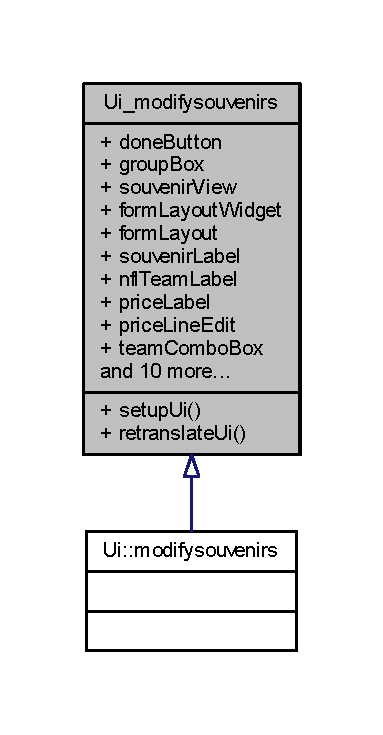
\includegraphics[width=184pt]{class_ui__modifysouvenirs__inherit__graph}
\end{center}
\end{figure}


Collaboration diagram for Ui\+\_\+modifysouvenirs\+:\nopagebreak
\begin{figure}[H]
\begin{center}
\leavevmode
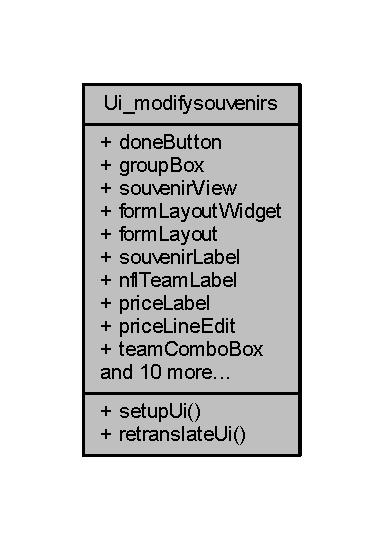
\includegraphics[width=184pt]{class_ui__modifysouvenirs__coll__graph}
\end{center}
\end{figure}
\subsection*{Public Member Functions}
\begin{DoxyCompactItemize}
\item 
\mbox{\Hypertarget{class_ui__modifysouvenirs_a65a331835a231045990275798a7e8df0}\label{class_ui__modifysouvenirs_a65a331835a231045990275798a7e8df0}} 
void {\bfseries setup\+Ui} (Q\+Dialog $\ast$\hyperlink{classmodifysouvenirs}{modifysouvenirs})
\item 
\mbox{\Hypertarget{class_ui__modifysouvenirs_a151a961dcf5b8f9a622d3d53619f8c35}\label{class_ui__modifysouvenirs_a151a961dcf5b8f9a622d3d53619f8c35}} 
void {\bfseries retranslate\+Ui} (Q\+Dialog $\ast$\hyperlink{classmodifysouvenirs}{modifysouvenirs})
\end{DoxyCompactItemize}
\subsection*{Public Attributes}
\begin{DoxyCompactItemize}
\item 
\mbox{\Hypertarget{class_ui__modifysouvenirs_a60f5031899d6d7c3d3fa2d708e829cbf}\label{class_ui__modifysouvenirs_a60f5031899d6d7c3d3fa2d708e829cbf}} 
Q\+Push\+Button $\ast$ {\bfseries done\+Button}
\item 
\mbox{\Hypertarget{class_ui__modifysouvenirs_af0a7ab1be760180cecd1ef407c12e0f2}\label{class_ui__modifysouvenirs_af0a7ab1be760180cecd1ef407c12e0f2}} 
Q\+Group\+Box $\ast$ {\bfseries group\+Box}
\item 
\mbox{\Hypertarget{class_ui__modifysouvenirs_a9d81bbb30cdc2c8ee7bb85c82ce10756}\label{class_ui__modifysouvenirs_a9d81bbb30cdc2c8ee7bb85c82ce10756}} 
Q\+Table\+View $\ast$ {\bfseries souvenir\+View}
\item 
\mbox{\Hypertarget{class_ui__modifysouvenirs_af15387c7b6c5cfd4b6b7702a935be905}\label{class_ui__modifysouvenirs_af15387c7b6c5cfd4b6b7702a935be905}} 
Q\+Widget $\ast$ {\bfseries form\+Layout\+Widget}
\item 
\mbox{\Hypertarget{class_ui__modifysouvenirs_ae4e06da7241d7cfcac77b5f04826f76e}\label{class_ui__modifysouvenirs_ae4e06da7241d7cfcac77b5f04826f76e}} 
Q\+Form\+Layout $\ast$ {\bfseries form\+Layout}
\item 
\mbox{\Hypertarget{class_ui__modifysouvenirs_a483cdb250d1c4d37828aceb33739220d}\label{class_ui__modifysouvenirs_a483cdb250d1c4d37828aceb33739220d}} 
Q\+Label $\ast$ {\bfseries souvenir\+Label}
\item 
\mbox{\Hypertarget{class_ui__modifysouvenirs_a1e38762b488bcd42341ae6c8b2d4f5f8}\label{class_ui__modifysouvenirs_a1e38762b488bcd42341ae6c8b2d4f5f8}} 
Q\+Label $\ast$ {\bfseries nfl\+Team\+Label}
\item 
\mbox{\Hypertarget{class_ui__modifysouvenirs_a3769911187bd25e386f61986b4451507}\label{class_ui__modifysouvenirs_a3769911187bd25e386f61986b4451507}} 
Q\+Label $\ast$ {\bfseries price\+Label}
\item 
\mbox{\Hypertarget{class_ui__modifysouvenirs_a6708f8618d5efc0d8d553d4125ea079b}\label{class_ui__modifysouvenirs_a6708f8618d5efc0d8d553d4125ea079b}} 
Q\+Line\+Edit $\ast$ {\bfseries price\+Line\+Edit}
\item 
\mbox{\Hypertarget{class_ui__modifysouvenirs_a22f560b28d46a2bd12fa20f4c9dcc1ec}\label{class_ui__modifysouvenirs_a22f560b28d46a2bd12fa20f4c9dcc1ec}} 
Q\+Combo\+Box $\ast$ {\bfseries team\+Combo\+Box}
\item 
\mbox{\Hypertarget{class_ui__modifysouvenirs_a36b6689d83cb203e609338792601610e}\label{class_ui__modifysouvenirs_a36b6689d83cb203e609338792601610e}} 
Q\+Combo\+Box $\ast$ {\bfseries souvenir\+Combo\+Box}
\item 
\mbox{\Hypertarget{class_ui__modifysouvenirs_a789bf12dd9c15b8bf55d0ceb7b91e1f6}\label{class_ui__modifysouvenirs_a789bf12dd9c15b8bf55d0ceb7b91e1f6}} 
Q\+Label $\ast$ {\bfseries new\+Souvenir\+Label}
\item 
\mbox{\Hypertarget{class_ui__modifysouvenirs_ac4d46d08e68d2bec4204a6b7204e919a}\label{class_ui__modifysouvenirs_ac4d46d08e68d2bec4204a6b7204e919a}} 
Q\+Line\+Edit $\ast$ {\bfseries new\+Souvenir\+Line\+Edit}
\item 
\mbox{\Hypertarget{class_ui__modifysouvenirs_a0200ccee44d6b2cd8595cc580ce4e58e}\label{class_ui__modifysouvenirs_a0200ccee44d6b2cd8595cc580ce4e58e}} 
Q\+Widget $\ast$ {\bfseries layout\+Widget}
\item 
\mbox{\Hypertarget{class_ui__modifysouvenirs_ad49cd42a8450e02d7cd2ba487bf96a62}\label{class_ui__modifysouvenirs_ad49cd42a8450e02d7cd2ba487bf96a62}} 
Q\+V\+Box\+Layout $\ast$ {\bfseries vertical\+Layout}
\item 
\mbox{\Hypertarget{class_ui__modifysouvenirs_a0ae86af68371d8cd99a2aeba4756ede1}\label{class_ui__modifysouvenirs_a0ae86af68371d8cd99a2aeba4756ede1}} 
Q\+Push\+Button $\ast$ {\bfseries delete\+Souvenir}
\item 
\mbox{\Hypertarget{class_ui__modifysouvenirs_aa1cbe1aab0166fc6a75ded347ddca9b8}\label{class_ui__modifysouvenirs_aa1cbe1aab0166fc6a75ded347ddca9b8}} 
Q\+Push\+Button $\ast$ {\bfseries modify\+Souvenir}
\item 
\mbox{\Hypertarget{class_ui__modifysouvenirs_a0bba50e69a604a5c5d6fee2daa76f43b}\label{class_ui__modifysouvenirs_a0bba50e69a604a5c5d6fee2daa76f43b}} 
Q\+Push\+Button $\ast$ {\bfseries add\+Souvenir}
\item 
\mbox{\Hypertarget{class_ui__modifysouvenirs_af3f05c3c14ddc0489b83439d13b3a681}\label{class_ui__modifysouvenirs_af3f05c3c14ddc0489b83439d13b3a681}} 
Q\+Group\+Box $\ast$ {\bfseries group\+Box\+\_\+2}
\item 
\mbox{\Hypertarget{class_ui__modifysouvenirs_ace4aba2b9ee276c4734f0f03ace8e565}\label{class_ui__modifysouvenirs_ace4aba2b9ee276c4734f0f03ace8e565}} 
Q\+Push\+Button $\ast$ {\bfseries add\+Sandiego\+Sailors\+Button}
\end{DoxyCompactItemize}


The documentation for this class was generated from the following file\+:\begin{DoxyCompactItemize}
\item 
ui\+\_\+modifysouvenirs.\+h\end{DoxyCompactItemize}

\hypertarget{class_ui__modify_stadium_info}{}\section{Ui\+\_\+modify\+Stadium\+Info Class Reference}
\label{class_ui__modify_stadium_info}\index{Ui\+\_\+modify\+Stadium\+Info@{Ui\+\_\+modify\+Stadium\+Info}}


Inheritance diagram for Ui\+\_\+modify\+Stadium\+Info\+:
\nopagebreak
\begin{figure}[H]
\begin{center}
\leavevmode
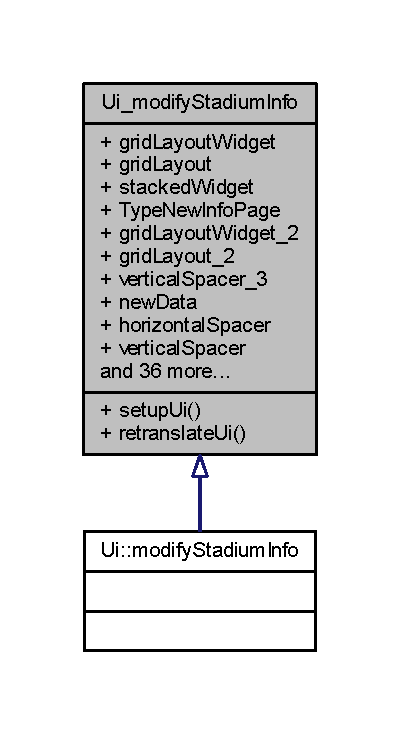
\includegraphics[width=192pt]{class_ui__modify_stadium_info__inherit__graph}
\end{center}
\end{figure}


Collaboration diagram for Ui\+\_\+modify\+Stadium\+Info\+:
\nopagebreak
\begin{figure}[H]
\begin{center}
\leavevmode
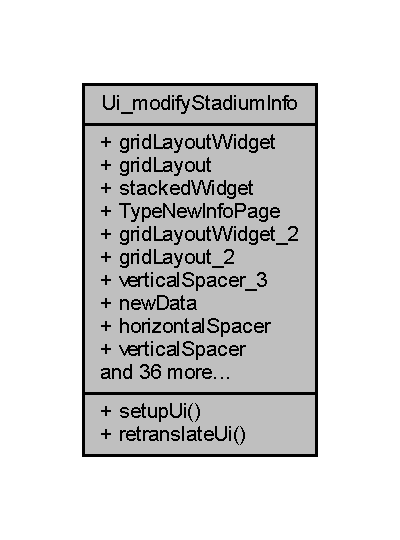
\includegraphics[width=192pt]{class_ui__modify_stadium_info__coll__graph}
\end{center}
\end{figure}
\subsection*{Public Member Functions}
\begin{DoxyCompactItemize}
\item 
\mbox{\Hypertarget{class_ui__modify_stadium_info_a1bc7fa7e327efff0a3686f47591c181f}\label{class_ui__modify_stadium_info_a1bc7fa7e327efff0a3686f47591c181f}} 
void {\bfseries setup\+Ui} (Q\+Dialog $\ast$\hyperlink{classmodify_stadium_info}{modify\+Stadium\+Info})
\item 
\mbox{\Hypertarget{class_ui__modify_stadium_info_a9c3a37f6edfa5d0a4515c32f7df62db2}\label{class_ui__modify_stadium_info_a9c3a37f6edfa5d0a4515c32f7df62db2}} 
void {\bfseries retranslate\+Ui} (Q\+Dialog $\ast$\hyperlink{classmodify_stadium_info}{modify\+Stadium\+Info})
\end{DoxyCompactItemize}
\subsection*{Public Attributes}
\begin{DoxyCompactItemize}
\item 
\mbox{\Hypertarget{class_ui__modify_stadium_info_a379932f80de2aac5829c27d1b7b6639a}\label{class_ui__modify_stadium_info_a379932f80de2aac5829c27d1b7b6639a}} 
Q\+Widget $\ast$ {\bfseries grid\+Layout\+Widget}
\item 
\mbox{\Hypertarget{class_ui__modify_stadium_info_a8473b0c692472487a8e4f3bb112e750c}\label{class_ui__modify_stadium_info_a8473b0c692472487a8e4f3bb112e750c}} 
Q\+Grid\+Layout $\ast$ {\bfseries grid\+Layout}
\item 
\mbox{\Hypertarget{class_ui__modify_stadium_info_a8c368a0a9537c6dd97cd3a1aa2918c9c}\label{class_ui__modify_stadium_info_a8c368a0a9537c6dd97cd3a1aa2918c9c}} 
Q\+Stacked\+Widget $\ast$ {\bfseries stacked\+Widget}
\item 
\mbox{\Hypertarget{class_ui__modify_stadium_info_a0be63e7aea444ed888f3cdbeb7fe6c26}\label{class_ui__modify_stadium_info_a0be63e7aea444ed888f3cdbeb7fe6c26}} 
Q\+Widget $\ast$ {\bfseries Type\+New\+Info\+Page}
\item 
\mbox{\Hypertarget{class_ui__modify_stadium_info_a5bd80cdcbcb8c23fa7c137d9031422d5}\label{class_ui__modify_stadium_info_a5bd80cdcbcb8c23fa7c137d9031422d5}} 
Q\+Widget $\ast$ {\bfseries grid\+Layout\+Widget\+\_\+2}
\item 
\mbox{\Hypertarget{class_ui__modify_stadium_info_a056000c4d80b31b72cae98dcb58bde73}\label{class_ui__modify_stadium_info_a056000c4d80b31b72cae98dcb58bde73}} 
Q\+Grid\+Layout $\ast$ {\bfseries grid\+Layout\+\_\+2}
\item 
\mbox{\Hypertarget{class_ui__modify_stadium_info_a6b2526b942b1381f3b74efca3dd6512f}\label{class_ui__modify_stadium_info_a6b2526b942b1381f3b74efca3dd6512f}} 
Q\+Spacer\+Item $\ast$ {\bfseries vertical\+Spacer\+\_\+3}
\item 
\mbox{\Hypertarget{class_ui__modify_stadium_info_a57f582d740f03a997ab16de47c875c9a}\label{class_ui__modify_stadium_info_a57f582d740f03a997ab16de47c875c9a}} 
Q\+Line\+Edit $\ast$ {\bfseries new\+Data}
\item 
\mbox{\Hypertarget{class_ui__modify_stadium_info_ab7b454e2e5290ed1b8a723b4603818fc}\label{class_ui__modify_stadium_info_ab7b454e2e5290ed1b8a723b4603818fc}} 
Q\+Spacer\+Item $\ast$ {\bfseries horizontal\+Spacer}
\item 
\mbox{\Hypertarget{class_ui__modify_stadium_info_af6f30027b065e66eb50141ea50cb2223}\label{class_ui__modify_stadium_info_af6f30027b065e66eb50141ea50cb2223}} 
Q\+Spacer\+Item $\ast$ {\bfseries vertical\+Spacer}
\item 
\mbox{\Hypertarget{class_ui__modify_stadium_info_a67aef7e9debc69d4a4d89c5abfada281}\label{class_ui__modify_stadium_info_a67aef7e9debc69d4a4d89c5abfada281}} 
Q\+Spacer\+Item $\ast$ {\bfseries horizontal\+Spacer\+\_\+2}
\item 
\mbox{\Hypertarget{class_ui__modify_stadium_info_ae9b5b3b0bfb784f722a9ae706ae4831f}\label{class_ui__modify_stadium_info_ae9b5b3b0bfb784f722a9ae706ae4831f}} 
Q\+H\+Box\+Layout $\ast$ {\bfseries horizontal\+Layout}
\item 
\mbox{\Hypertarget{class_ui__modify_stadium_info_afd77e8d611278f1c38cfbb448e1f1ab8}\label{class_ui__modify_stadium_info_afd77e8d611278f1c38cfbb448e1f1ab8}} 
Q\+Push\+Button $\ast$ {\bfseries push\+Button\+\_\+2}
\item 
\mbox{\Hypertarget{class_ui__modify_stadium_info_a81b582dbfc3518a0fdb9180e39411597}\label{class_ui__modify_stadium_info_a81b582dbfc3518a0fdb9180e39411597}} 
Q\+Spacer\+Item $\ast$ {\bfseries horizontal\+Spacer\+\_\+3}
\item 
\mbox{\Hypertarget{class_ui__modify_stadium_info_aaa1ae45cf262b2017ea0e62776724992}\label{class_ui__modify_stadium_info_aaa1ae45cf262b2017ea0e62776724992}} 
Q\+Push\+Button $\ast$ {\bfseries P\+B\+\_\+\+Update}
\item 
\mbox{\Hypertarget{class_ui__modify_stadium_info_a859842e665a398bec11b7feec41c6811}\label{class_ui__modify_stadium_info_a859842e665a398bec11b7feec41c6811}} 
Q\+Label $\ast$ {\bfseries column\+Name}
\item 
\mbox{\Hypertarget{class_ui__modify_stadium_info_a913ab576de1c663c892d22c462be5d69}\label{class_ui__modify_stadium_info_a913ab576de1c663c892d22c462be5d69}} 
Q\+Spacer\+Item $\ast$ {\bfseries vertical\+Spacer\+\_\+2}
\item 
\mbox{\Hypertarget{class_ui__modify_stadium_info_ada0e602115efcec941720a524d178ca0}\label{class_ui__modify_stadium_info_ada0e602115efcec941720a524d178ca0}} 
Q\+Spacer\+Item $\ast$ {\bfseries vertical\+Spacer\+\_\+4}
\item 
\mbox{\Hypertarget{class_ui__modify_stadium_info_a554cec79fed48bfff454b3f009b9d409}\label{class_ui__modify_stadium_info_a554cec79fed48bfff454b3f009b9d409}} 
Q\+Widget $\ast$ {\bfseries Click\+Page}
\item 
\mbox{\Hypertarget{class_ui__modify_stadium_info_a6ad834791c8d28131eb2ddbf53aa7c88}\label{class_ui__modify_stadium_info_a6ad834791c8d28131eb2ddbf53aa7c88}} 
Q\+Widget $\ast$ {\bfseries grid\+Layout\+Widget\+\_\+3}
\item 
\mbox{\Hypertarget{class_ui__modify_stadium_info_a2528083bd497541de1527de8b17f167a}\label{class_ui__modify_stadium_info_a2528083bd497541de1527de8b17f167a}} 
Q\+Grid\+Layout $\ast$ {\bfseries grid\+Layout\+\_\+3}
\item 
\mbox{\Hypertarget{class_ui__modify_stadium_info_af7efdd50156d2bf4e036e9b339d8853f}\label{class_ui__modify_stadium_info_af7efdd50156d2bf4e036e9b339d8853f}} 
Q\+Combo\+Box $\ast$ {\bfseries combo\+Box}
\item 
\mbox{\Hypertarget{class_ui__modify_stadium_info_a22398185bcb0d14052d60226b6e0a836}\label{class_ui__modify_stadium_info_a22398185bcb0d14052d60226b6e0a836}} 
Q\+H\+Box\+Layout $\ast$ {\bfseries horizontal\+Layout\+\_\+2}
\item 
\mbox{\Hypertarget{class_ui__modify_stadium_info_a96029215bda56113c7a72c35e9e58137}\label{class_ui__modify_stadium_info_a96029215bda56113c7a72c35e9e58137}} 
Q\+Push\+Button $\ast$ {\bfseries push\+Button\+\_\+3}
\item 
\mbox{\Hypertarget{class_ui__modify_stadium_info_ab4f36653e8fbf74b3ae106e624334727}\label{class_ui__modify_stadium_info_ab4f36653e8fbf74b3ae106e624334727}} 
Q\+Spacer\+Item $\ast$ {\bfseries horizontal\+Spacer\+\_\+6}
\item 
\mbox{\Hypertarget{class_ui__modify_stadium_info_ac1e0844f985344205154f73192d96654}\label{class_ui__modify_stadium_info_ac1e0844f985344205154f73192d96654}} 
Q\+Push\+Button $\ast$ {\bfseries push\+Button}
\item 
\mbox{\Hypertarget{class_ui__modify_stadium_info_ad49b5e70d0de6e835714caac3fb34bc6}\label{class_ui__modify_stadium_info_ad49b5e70d0de6e835714caac3fb34bc6}} 
Q\+Spacer\+Item $\ast$ {\bfseries vertical\+Spacer\+\_\+7}
\item 
\mbox{\Hypertarget{class_ui__modify_stadium_info_ad794dcbf43f3f402a7f23d8dc00b4a8a}\label{class_ui__modify_stadium_info_ad794dcbf43f3f402a7f23d8dc00b4a8a}} 
Q\+Spacer\+Item $\ast$ {\bfseries vertical\+Spacer\+\_\+5}
\item 
\mbox{\Hypertarget{class_ui__modify_stadium_info_a508c5c046f2026153607ddb5d42947f3}\label{class_ui__modify_stadium_info_a508c5c046f2026153607ddb5d42947f3}} 
Q\+Spacer\+Item $\ast$ {\bfseries vertical\+Spacer\+\_\+6}
\item 
\mbox{\Hypertarget{class_ui__modify_stadium_info_aa21a30cb4dc156708ba133b34bf29d54}\label{class_ui__modify_stadium_info_aa21a30cb4dc156708ba133b34bf29d54}} 
Q\+Spacer\+Item $\ast$ {\bfseries horizontal\+Spacer\+\_\+4}
\item 
\mbox{\Hypertarget{class_ui__modify_stadium_info_abc440ea8e3afd9265dd1f9bdd06d2a09}\label{class_ui__modify_stadium_info_abc440ea8e3afd9265dd1f9bdd06d2a09}} 
Q\+Label $\ast$ {\bfseries label\+\_\+drop\+Down\+Header}
\item 
\mbox{\Hypertarget{class_ui__modify_stadium_info_a5d42d8066bb3310bf2ded3feaaa11375}\label{class_ui__modify_stadium_info_a5d42d8066bb3310bf2ded3feaaa11375}} 
Q\+Spacer\+Item $\ast$ {\bfseries horizontal\+Spacer\+\_\+5}
\item 
\mbox{\Hypertarget{class_ui__modify_stadium_info_adb325bf46b0395cf44cdb498970fa6c3}\label{class_ui__modify_stadium_info_adb325bf46b0395cf44cdb498970fa6c3}} 
Q\+Spacer\+Item $\ast$ {\bfseries vertical\+Spacer\+\_\+8}
\item 
\mbox{\Hypertarget{class_ui__modify_stadium_info_a3a1a5b83a3cb25b33b5a128e640f7941}\label{class_ui__modify_stadium_info_a3a1a5b83a3cb25b33b5a128e640f7941}} 
Q\+Widget $\ast$ {\bfseries Conference\+Page}
\item 
\mbox{\Hypertarget{class_ui__modify_stadium_info_acde3d07f59c61065cd59b4cf61f18ad6}\label{class_ui__modify_stadium_info_acde3d07f59c61065cd59b4cf61f18ad6}} 
Q\+Widget $\ast$ {\bfseries grid\+Layout\+Widget\+\_\+4}
\item 
\mbox{\Hypertarget{class_ui__modify_stadium_info_a3941a4019a9d1ecdd6b852119b4577c1}\label{class_ui__modify_stadium_info_a3941a4019a9d1ecdd6b852119b4577c1}} 
Q\+Grid\+Layout $\ast$ {\bfseries grid\+Layout\+\_\+4}
\item 
\mbox{\Hypertarget{class_ui__modify_stadium_info_a406dfe7c2098b8a8613d23fa4f201690}\label{class_ui__modify_stadium_info_a406dfe7c2098b8a8613d23fa4f201690}} 
Q\+Spacer\+Item $\ast$ {\bfseries horizontal\+Spacer\+\_\+8}
\item 
\mbox{\Hypertarget{class_ui__modify_stadium_info_a8ebeb616e4adbf2b9c62d91aab644f01}\label{class_ui__modify_stadium_info_a8ebeb616e4adbf2b9c62d91aab644f01}} 
Q\+Spacer\+Item $\ast$ {\bfseries horizontal\+Spacer\+\_\+7}
\item 
\mbox{\Hypertarget{class_ui__modify_stadium_info_a83d6573348ebec76b3413ab945d62940}\label{class_ui__modify_stadium_info_a83d6573348ebec76b3413ab945d62940}} 
Q\+Spacer\+Item $\ast$ {\bfseries vertical\+Spacer\+\_\+9}
\item 
\mbox{\Hypertarget{class_ui__modify_stadium_info_ade64b2296f768c37b1b54d18f95df2fa}\label{class_ui__modify_stadium_info_ade64b2296f768c37b1b54d18f95df2fa}} 
Q\+H\+Box\+Layout $\ast$ {\bfseries horizontal\+Layout\+\_\+3}
\item 
\mbox{\Hypertarget{class_ui__modify_stadium_info_a98dd83cf73cb27d2eefc51c5219fba70}\label{class_ui__modify_stadium_info_a98dd83cf73cb27d2eefc51c5219fba70}} 
Q\+Push\+Button $\ast$ {\bfseries cancel\+\_\+conference}
\item 
\mbox{\Hypertarget{class_ui__modify_stadium_info_a5b5020c30a62838402ce07b07e73692b}\label{class_ui__modify_stadium_info_a5b5020c30a62838402ce07b07e73692b}} 
Q\+Spacer\+Item $\ast$ {\bfseries horizontal\+Spacer\+\_\+9}
\item 
\mbox{\Hypertarget{class_ui__modify_stadium_info_a1bc42e5244bea86b3e51aadaaf998724}\label{class_ui__modify_stadium_info_a1bc42e5244bea86b3e51aadaaf998724}} 
Q\+Push\+Button $\ast$ {\bfseries P\+B\+\_\+\+Conference}
\item 
\mbox{\Hypertarget{class_ui__modify_stadium_info_a49f3f4a1c6f222cf336974a5143552ba}\label{class_ui__modify_stadium_info_a49f3f4a1c6f222cf336974a5143552ba}} 
Q\+Label $\ast$ {\bfseries conference\+\_\+label}
\item 
\mbox{\Hypertarget{class_ui__modify_stadium_info_a6c2eff8ebcc565138255e0836fec87e8}\label{class_ui__modify_stadium_info_a6c2eff8ebcc565138255e0836fec87e8}} 
Q\+Spacer\+Item $\ast$ {\bfseries vertical\+Spacer\+\_\+10}
\item 
\mbox{\Hypertarget{class_ui__modify_stadium_info_a186080de3650503d33ad86a73389835b}\label{class_ui__modify_stadium_info_a186080de3650503d33ad86a73389835b}} 
Q\+Spacer\+Item $\ast$ {\bfseries vertical\+Spacer\+\_\+11}
\end{DoxyCompactItemize}


The documentation for this class was generated from the following file\+:\begin{DoxyCompactItemize}
\item 
ui\+\_\+modifystadiuminfo.\+h\end{DoxyCompactItemize}

\hypertarget{struct_vertex}{}\section{Vertex Struct Reference}
\label{struct_vertex}\index{Vertex@{Vertex}}


Used to represent a \hyperlink{struct_vertex}{Vertex} for the graph class.  




{\ttfamily \#include $<$graph.\+h$>$}



Collaboration diagram for Vertex\+:
\nopagebreak
\begin{figure}[H]
\begin{center}
\leavevmode
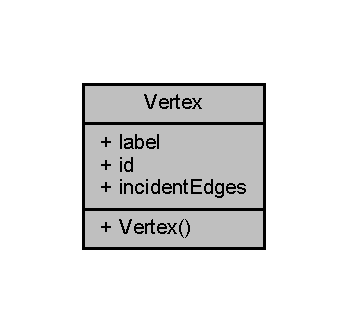
\includegraphics[width=167pt]{struct_vertex__coll__graph}
\end{center}
\end{figure}
\subsection*{Public Attributes}
\begin{DoxyCompactItemize}
\item 
\mbox{\Hypertarget{struct_vertex_a60447a604e4decc34e1ef4f89909ac97}\label{struct_vertex_a60447a604e4decc34e1ef4f89909ac97}} 
Q\+String {\bfseries label}
\item 
\mbox{\Hypertarget{struct_vertex_a2e69697726190f50c7fc040fb1ddac7a}\label{struct_vertex_a2e69697726190f50c7fc040fb1ddac7a}} 
int {\bfseries id}
\item 
\mbox{\Hypertarget{struct_vertex_a925bd1413228b69ba059c58bfa96b43c}\label{struct_vertex_a925bd1413228b69ba059c58bfa96b43c}} 
Q\+Vector$<$ \hyperlink{struct_edge}{Edge} $>$ {\bfseries incident\+Edges}
\end{DoxyCompactItemize}


\subsection{Detailed Description}
Used to represent a \hyperlink{struct_vertex}{Vertex} for the graph class. 

This struct represents a vertex for the graph. It has a label, unique ID, and a vector of incident edges. 

The documentation for this struct was generated from the following file\+:\begin{DoxyCompactItemize}
\item 
graph.\+h\end{DoxyCompactItemize}

%--- End generated contents ---

% Index
\backmatter
\newpage
\phantomsection
\clearemptydoublepage
\addcontentsline{toc}{chapter}{Index}
\printindex

\end{document}
